\documentclass[11pt]{article}
\usepackage[left=1in,top=1in,right=1in,bottom=1in,head=0in,nofoot]{geometry}

\setlength{\footskip}{24pt} % Page number/footer spacing
\usepackage{setspace,url,bm,amsmath} % For double-spacing, URL font, math symbols
\usepackage{scalerel}
\newcommand{\bbb}{\mathbf }
\usepackage{xcolor}
 \usepackage{multirow}
 \usepackage{arydshln}
 \usepackage{mathtools}
\usepackage{titlesec} % Section header formatting
\titlelabel{\thetitle.\quad} % Section header formatting
%\titleformat*{\section}{\bf\large\center\uppercase} % Section header formatting
\titleformat*{\section}{\bf\Large\center}

\usepackage{float}
\usepackage{graphicx} % Graphics scaling
\usepackage{bbm}
\usepackage{latexsym}
\usepackage{caption}
\usepackage[margin=20pt]{subcaption}
\usepackage{enumerate}

\def\prg{\medskip\noindent\textbf}
\def\mtas{{multi-armed }}
\def\mes{{multi-armed experiments}}
\def\mess{{multi-armed experiments }}
\def\tosrp{\tilde\Omega_{*,\rr,\pp}}
\def\hybr{\hy\la \hbr\ra}
\def\hybsr{\hy\la\hbsr\ra}
\def\hybrs{ \hy\la\hbrs\ra}
\def\hybs{\hy\la b_*\ra}
\def\hybi{\hy\la \bi \ra}
\def\hyba{\hy\la b \ra}
\def\la{\langle}
\def\ra{\rangle}
\def\hsxy{\hat S_{xY}}\def\gt{\Gamma^\T}
\def\her{\hep_\rr}
\def\rpp{R_\perp}
\def\rpt{R^\T_\perp}
\def\xcc{(X_1, \ldots, X_{Q})}
\def\xpp{(X_1 + \cdots + X_{Q})}
\def\lhs{\textsc{lhs}}
\def\rhs{\textsc{rhs}}
\def\iln{(1_n^\T \otimes \il)}
\def\ilnt{(1_n\otimes \il)} %\beginp \il \\ \vdots \\ \il \endp}
\def\ill{(\il, \il)}
\def\rge{(-\il, \il)}
\def\illt{\beginp \il\\ \il\endp}
\def\rgte {\beginp -\il\\ \il\endp}
\def\dto{\Delta_1}
\def\ar{A_\rr}
\def\br{B_\rr}\def\xxinv{(X^\T X)^{-1}}
\def\xx{X^\T X}
\def\il{I_l}\def\xot{X_1^\T}
\def\xtt{X_2^\T}
\def\xtht{X_3^\T}
\def\xt{X_2}
\def\xth{X_3}
\def\soo{S_{11}}
\def\stt{S_{22}}
\def\sto{S_{21}}
\def\sot{S_{12}}

\def\dt{\Delta}\def\hsrs{\hat\Psi_{\rr,*}}
\def\ccinvs{(\chi_*^\T\chi_*)^{-1}}
\def\Ms{M_*}
\def\murq{\mu_{\rr,q}}
\def\hvr{\hat V_\rr}
\def\tgginv{\tgg^{-1}}
\def\hsig{\hat\Sigma}
\def\hsigr{\hsig_\rr}
\def\hsigrq{(\hsigr)_{[Q]}}
\def\hsis{\hsi_*}
\def\hesi{\hep_{*,i}}
\def\neqinv{N_q^{-1}}\def\hsxq{\hat S^2_x(q)}
\def\hsxyq{\hat S_{xY(q)}}
\def\tgg{{\red \tilde\Gamma}}
\def\qit{{q\in\mt}}\def\txi{\tilde{\xi}}
\def\fa{A}
\def\torpp{{\red \torp'}}
\def\topp{{\red \top'}}
\def\tmu{\tilde\mu}
\def\tetp{\tilde{\eta}_\pp}
\def\tetm{\tilde{\eta}_\mmm}
\def\tmur{\tilde\mu_\rr}
\def\tetrp{\tilde{\eta}_{\rr,\pp}}
\def\tetrm{\tilde{\eta}_{\rr,\mmm}}

\def\nllinv{(\ninv\lmdpt\lmdp)^{-1}}
\def\nffinv{(\ninv\fpt\fpp)^{-1}}
\def\ninv{N^{-1}}
\def\cspt{\csp^\T}
\def\csmt{\csm^\T}
\def\tcspt{\tcsp^\T}
\def\tcsp{\tilde C_{\sss,\pp}}
\def\ft{F^\T}
\def\piinv{\Pi^{-1}}
\def\gsinv{\gs^{-1}}
\def\gst{\gs^\T}
\def\fmt{\fm^\T}
\def\mlr{M_{\lin,\rr}}
\def\fpq{f_{\pp(q)}}
\def\fmq{f_{\mmm(q)}}
\def\gs{\Gamma_\sss}
\def\tsigr{\tilde\Sigma_\rr}\def\trr{\tilde R}
\def\tchil{\tilde\chi_\lin}
\def\tcl{\tilde\chi_\lin}
\def\tmr{\tilde M_\rr}
\def\chil{\chi_\lin}
\def\cse{c_{\sss,\emptyset}}\def\tsig{\tilde\Sigma}
\def\tsigp{\tilde\Sigma_\pp}
\def\tsigrp{\tilde\Sigma_{\rr,\pp}}
\def\wheret{\qquad\text{where} \ \ }
\def\lmdm{\Lambda_\mmm}
\def\tsigl{\tilde\Sigma_\lin}
\def\fm{F_\mmm}
\def\fmi{f_{\mmm,i}}
\def\xm{X_\mmm}
\def\lmdp{\Lambda_\pp}
\def\lmdpt{\Lambda_\pp^\T}
\def\xp{X_\pp}
\def\xpt{X_\pp^\T}
\def\xmt{X_\mmm^\T}
\def\tthrp{\tilde\theta_{\rr,\pp}}
\def\tthp{\tilde\theta_{\pp}}
\def\tthm{\tilde\theta_{\mmm}}

\def\ttp{\ttau_\pp}
\def\ttm{\ttau_\mmm}
\def\tol{\tilde\Omega_\lin}
\def\fpp{F_\pp}
\def\fpi{f_{\pp,i}}
\def\fpt{\fpp^\T}
\def\hbro{\hb_{\rr,1}}
\def\tepr{\tep_{\rr}}
\def\tepri{\tep_{\rr,i}}
\def\hepr{\hep_{\rr}}
\def\hepri{\hep_{\rr,i}}
\def\tepi{\tep_i}
\def\tep{\tilde\epsilon}
\def\hV{\hv}
\def\hvro{\hv_{\rr,1}}
\def\top{\tilde\Omega_\pp}
\def\tgd{\ttrp}

\def\rb{A}
\def\mub{B}
\def\apo{average potential outcomes}
\def\cpoc{correlations between potential outcomes and covariates}\def\tsyx{\hat S_{Yx}} 
\def\gray{\color{gray}}
\def\torp{\tilde \Omega_{\rr,\pp}}
\def\zikz{\zik^0}
\def\zimkz{\zimk^0}

\def\ust{\us^\T}
\def\co{\go}
\def\poo{potential-outcome-only}
\def\go{correlation-only}
\def\gor{correlation-only restriction}
\def\so{separable}
\def\sor{separable restriction}
\def\sr{separable restriction}
\def\tss{S'}
\def\yc{\hy}
 \def\ppo{{\scaleto{+}{6pt}}}
 \def\mmz{{\scaleto{-}{6pt}}}
 \def\pmo{\{-1, +1\}}
\def\hylr{\hy_{\lin,\rr}}
\def\hyfr{\hy_{\fisher,\rr}}
\def\hynr{\hy_{\nm,\rr}}

\def\ttrp{\tilde\tau_{\rr,\pp}}
\def\ttrm{\tilde\tau_{\rr,\mmm}}
\def\ttrmk{\ttau_{\rr,\mk}}
\def\ttsp{\ttau_{*,\pp}}
\def\ttnp{\ttau_{\nm,\pp}}
\def\ttfp{\ttau_{\fisher,\pp}}
\def\ttlp{\ttau_{\lin,\pp}}

\def\ttsrp{\ttau_{*,\rr,\pp}}
\def\ttnrp{\ttau_{\nm,\rr,\pp}}
\def\tts{\ttau_{*}}
\def\ttn{\ttau_{\neyman}}
\def\ttf{\ttau_{\fisher}}
\def\ttl{\ttau_{\lin}}


\def\ttfrp{\ttau _{\fisher, \rr,\pp}}
\def\ttnrp{\ttau _{\neyman, \rr,\pp}}
\def\ttlrp{\ttau _{\lin,\rr ,\pp}}
\def\ttsrp{\ttau _{*, \rr,\pp}}
\def\tq{t_{(q)}}


\def\ttsmk{\ttau_{*, \mk}}
\def\ttnmk{\ttau_{\nm, \mk}}
\def\ttfmk{\ttau_{\fisher, \mk}}
\def\ttlmk{\ttau_{\lin, \mk}}

\def\ttnrmk{\ttau_{\nm, \rr,\mk}}
\def\ttfrmk{\ttau_{\fisher, \rr,\mk}}
\def\ttlrmk{\ttau_{\lin, \rr, \mk}}


\def\ttsrmk{\ttau_{*, \rr, \mk}}
\def\ttau{\tilde\tau}
%\def\htplp{\htau_{\rr,\pp}^0}
\def\murs{\mu_{\rr,\sss}}
\def\us{U_\sss}
\def\vrrs{V_{\rr,\sss}}
\def\hvs{\hat V_*}
\def\tos{\tilde \Omega_*}
\def\ca{c_\A}
\def\cb{c_\B}
\def\cab{c_\AB}
\def\csk{\cmk}
\def\cmk{c_\mk}
\def\ndt{non-degenerate linear transformation of the  regressor vector}
\def\hyrz{\hy_{\rr,0}}
\def\hbrz{\hb_{\rr,0}}
\def\hyrs{\hy_{\rr,\sss}}
\def\hbrs{\hb_{\rr,\sss}}
\def\brsq{\beta_{\rr,\sss,q}}
\def\hbrsq{\hb_{\rr,\sss,q}}
\def\kik{{k\in\mk}}
\def\ziks{\zik^\sss}
\def\zik{Z_{ik}}
\def\zimks{\zimk}
\def\htzrmk{\tilde\tau^0_{\rr,\mk}}
\def\htzrp{\tilde\tau^0_{\rr,\pp}}

\def\cza{c_{0, \A}}
\def\czb{c_{0, \B}}
\def\czab{c_{0, \AB}}
\def\tabz{\tau_{0,\AB}}
\def\htz{\tilde \tau^0}
\def\tz{\tau_0}
\def\tzp{\tau_{0,\pp}}
\def\tzm{\tau_{0,\mmm}}
\def\czm{C_{0,\mmm}}
\def\czmk{c_{0, \mk}}

%\def\tsmk{\tau_{\sss,\mk}}
%\def\tsm{\tau_{\sss,\mmm}}
\def\tsmk{\tau_{\mk}}
\def\tsm{\tau_{\sss,\mmm}}

\def\csmt{C^\T_{\sss,\mmm}}
\def\csm{C_{\sss,\mmm}}
\def\csmk{c_{\sss, \mk}}


\def\tzmk{\tau_{0, \mk}}

\def\epni{\ep_{\neyman,i}}
\def\vrr{V_\rr}

\def\cst{C_\sss^\T}
\def\cs{C_\sss}
\def\csp{C_{\sss,\pp}}
\def\ts{\tau_\sss}
\def\tsp{\tau_{\sss,\pp}}
\def\ta{\tau_\A}
\def\tb{\tau_\B}
\def\tp{\tau_\pp}

\def\htq{\htau^\sss }
\def\htqfrp{\htau^\sss _{\fisher, \rr,\pp}}
\def\htqnrp{\htau^\sss _{\neyman, \rr,\pp}}
\def\htqlrp{\htau^\sss _{\lin,\rr ,\pp}}
\def\htqsrp{\htau^\sss _{*, \rr,\pp}}

\def\htqfp{\htau^\sss _{\fisher, \pp}}
\def\htqnp{\htau^\sss _{\neyman, \pp}}
\def\htqlp{\htau^\sss _{\lin,\pp}}
\def\htqsp{\htau^\sss _{*,\pp}}

\def\htqnra{\htau^\sss _{\nm, \rr,\A}}
\def\htqfra{\htau^\sss _{\fisher, \rr,\A}}
\def\htqlra{\htau^\sss _{\llr ,\A}}
\def\htqsra{\htau^\sss _{*, \rr,\A}}

\def\htqnrb{\htau^\sss _{\nm, \rr,\B}}
\def\htqfrb{\htau^\sss _{\fisher, \rr,\B}}
\def\htqlrb{\htau^\sss _{\llr ,\B}}
\def\htqsrb{\htau^\sss _{*, \rr,\B}}

\def\htqsrp{\htau^\sss _{*,\rr,\pp}}
\def\htqsp{\htau^\sss _{*,\pp}}

\def\htqnmk{\htq_{\nm, \mk}}
\def\htqfmk{\htq_{\fisher, \mk}}
\def\htqlmk{\htq_{\lin, \mk}}
\def\htqsmk{\htq_{*, \mk}}

\def\htqnrmk{\htq_{\nm, \rr, \mk}}
\def\htqfrmk{\htq_{\fisher, \rr, \mk}}
\def\htqlrmk{\htq_{\llr , \mk}}
\def\htqsrmk{\htq_{*, \rr, \mk}}

\def\htql{\htau^\sss _\lin}
\def\htqf{\htau^\sss _\fisher}
\def\htqn{\htau^\sss _\neyman}
\def\htqlr{\htau^\sss _{\lr }}
\def\htqfr{\htau^\sss _{\fisher,\rr}}
\def\htqfrp{\htau^\sss _{\fisher,\rr,\pp}}
\def\htqfp{\htau^\sss _{\fisher,\pp}}
\def\htqs{\htau^\sss _*}
\def\htqsr{\htau^\sss _{*,\rr}}

\def\htp{\tilde\tau^0 }
\def\htpfrp{\htz _{\fisher, \rr,\pp}}
\def\htpnrp{\htz _{\neyman, \rr,\pp}}
\def\htplrp{\htz _{\lin,\rr ,\pp}}
\def\htpsrp{\htz _{*, \rr,\pp}}

\def\htpfp{\htz _{\fisher, \pp}}
\def\htpnp{\htz _{\neyman, \pp}}
\def\htplp{\htz _{\lin,\pp}}
\def\htpsp{\htz _{*,\pp}}

\def\htpnra{\htz _{\nm, \rr,\A}}
\def\htpfra{\htz _{\fisher, \rr,\A}}
\def\htplra{\htz _{\llr ,\A}}
\def\htpsra{\htz _{*, \rr,\A}}

\def\htpnrb{\htz _{\nm, \rr,\B}}
\def\htpfrb{\htz _{\fisher, \rr,\B}}
\def\htplrb{\htz _{\llr ,\B}}
\def\htpsrb{\htz _{*, \rr,\B}}

\def\htpsrp{\htz _{*,\rr,\pp}}
\def\htpsp{\htz _{*,\pp}}

\def\htpnmk{\htp_{\nm, \mk}}
\def\htpfmk{\htp_{\fisher, \mk}}
\def\htplmk{\htp_{\lin, \mk}}
\def\htpsmk{\htp_{*, \mk}}

\def\htpnrmk{\htp_{\nm, \rr, \mk}}
\def\htpfrmk{\htp_{\fisher, \rr, \mk}}
\def\htplrmk{\htp_{\llr , \mk}}
\def\htpsrmk{\htp_{*, \rr, \mk}}

\def\htpl{\htz _\lin}
\def\htpf{\htz _\fisher}
\def\htpn{\htz _\neyman}
\def\htplr{\htz _{\lr }}
\def\htpfr{\htz _{\fisher,\rr}}
\def\htpfrp{\htz _{\fisher,\rr,\pp}}
\def\htpfp{\htz _{\fisher,\pp}}
\def\htps{\htz _*}
\def\htpsr{\htz _{*,\rr}}

\def\ais{A_i^\textsc{s}}
\def\bis{B_i^\textsc{s}}
\def\sss{{\textsc{s}}}
\def\tauA{\ta}
\def\tauB{\tb}
\def\tab{\tau_\AB}
\def\taz{\tau_{0,\A}}
\def\tbz{\tau_{0, \B}}
\def\black{\color{black}}
\def\taua{\tau_\A}
\def\taub{\tau_\B}
\def\tauab{\tau_\AB}
\def\mrm{\mathbb R^m}
\def\mc{\mathcal C}
\def\ccf{\chif^\T\chif}
\def\preci{\preceq_\infty}
\def\opo{\Op(1)}
\def\oo{O(1)}
\def\ei{E_\infty}
\def\covi{\cov_\infty}
%\def\ei{E_\textup{a}}
%\def\covi{\cov_\textup{a}}

\def\uf{U_\fisher}
\def\rgp{R_{\gp}}
\def\rhgp{\rho_{\gp}}
\def\brq{\beta_{\rr,q}}
\def\xir{\xi_\rr}
\def\xiri{\xi_{\rr,\infty}}
\def\ary{A\rhy}
%\def\cxi{(x_i - \bx)}
%\def\cxi{x_{i, \textup{c}}}
\def\cxi{x_i}

\def\aryt{\rhy^\T A^\T}
 
\def\lr{{\rr}}
 

\def\ecc{the equal correlation condition}
\def\zcc{the zero correlation condition}
\def\eccs{{the equal correlation condition} }
\def\zccs{{the zero correlation condition} }
\def\czmk{c_{0, \mk}}
\def\htsss{\htau_{**}}
\def\xxx{\text{\red xxx} }
\def\ho{\hat\Omega}
\def\hsigl{\hat\Sigma_\lin}
\def\hsigf{\hat\Sigma_\fisher}
\def\hsigs{\hat\Sigma_*}
\def\hsiglr{\hat\Sigma_{\lr }}
\def\heli{\hat\ep_{\lin,i}}
\def\heri{\hat\ep_{\rr,i}}
\def\helri{\hat\ep_{\lr ,i}}
\def\hefi{\hat\ep_{\fisher,i}}
\def\heni{\hat\ep_{\nm,i}}
\def\chin{\chi_\nm}


\def\hsl{\hat\Psi_\lin}
\def\hsf{\hat\Psi_\fisher}
\def\hsn{\hat\Psi_\nm}
\def\hslr{\hat\Psi_{\lr }}
\def\hsr{\hsi_\rr}

\def\rhypt{\rhy^\T}
\def\tgmk{\tau_{\gamma, \mk}}
\def\czp{C_{0, \pp}}
\def\cz{C_0}



\def\pk{\mathcal P_K}
\def\mfm{\mathcal F_\mmm}
\def\mfp{\mathcal F_\pp}
\def\mfpp{\mathcal F_\pp'}
\def\tpp{\tau_\pp}
\def\tmk{\tau_\mk}
\def\tauabz{\tau_\abz}
\def\tauAB{\tau_\AB}
\def\taubaz{\tau_\baz}

\def\lrp{{\lr ,\pp}}
\def\frp{{\fisher, \rr,\pp}}
\def\nrp{{\neyman, \rr,\pp}}

\def\lp{{\lin, \pp}}
\def\fp{{\fisher, \pp}}
\def\np{{\neyman, \pp}}



\def\reslp{(R\tl - r)}
\def\resl{R\tl - r}
\def\resfp{(R\tf - r)}
\def\resf{R\tf - r}

 
\def\mulr{\mu_{\lin, \rr}} 
\def\mufr{\mu_{\fisher, \rr}} 
\def\munr{\mu_{\nm, \rr}} 

\def\muri{\mu_{\lr ,\infty}}
\def\mur{\mu_{\lr }}
\def\blr{\beta_{\lr }}
\def\htna{\htz _{\neyman,\A}}
\def\htnb{\htz _{\neyman,\B}}
\def\htnab{\htz _{\neyman,\AB}}
\def\htnra{\htz _{\neyman,\rr,\A}}
\def\htnrb{\htz _{\neyman,\rr,\B}}
\def\htnrab{\htz _{\neyman,\rr,\AB}}

\def\htfa{\htz _{\fisher,\A}}
\def\htfb{\htz _{\fisher,\B}}
\def\htfab{\htz _{\fisher,\AB}}
\def\htfra{\htz _{\fisher,\rr,\A}}
\def\htfrb{\htz _{\fisher,\rr,\B}}
\def\htfrab{\htz _{\fisher,\rr,\AB}}

\def\zimk{Z_{i, \mk}}
\def\htla{\htz _{\lin,\A}}
\def\htlb{\htz _{\lin,\B}}
\def\htlab{\htz _{\lin,\AB}}
\def\llr{\lin,\rr}
\def\htlra{\htz _{\llr ,\A}}
\def\htlrb{\htz _{\llr ,\B}}
\def\htlrab{\htz _{\llr ,\AB}}


\def\ad{& +}

%\def\rols{r-\ols}
%\def\rolss{r-\olss}
\def\rols{\rls}
\def\rolss{\rlss}
\def\rls{\textsc{rls}}
\def\rlss{{\textsc{rls} }}

\def\rolsf{restricted {\ols}}
\def\rolssf{restricted {\olss}}


\def\dy{\Delta_Y}
\def\dyf{\Delta_{Y, \fisher}}
\def\dgf{\Delta_{\gamma, \fisher}}

\def\mb{\mathcal{B}}
\def\vlr{V_\rr}
\def\vrr{V_\rr}
\def\vfr{V_{\fisher,\rr}}
\def\tf{\theta_\fisher}
\def\uy{U_Y}
\def\uyt{U_Y^\T}
\def\eqq{\, &= \,}
\def\simm{\, &\sim \,}
\def\dz{\Delta_0}
\def\es{\emat\otimes\sxx}
\def\esinv{(\es)^{-1}}
\def\ry{R_Y}
\def\rg{R_\gamma}
\def\rhy{\rho_Y}
\def\rys{r_{Y,*}}
\def\rhys{\rho_{Y,*}}
\def\rhyn{\rho_{Y, \neyman}}
\def\rhyf{\rho_{Y, \fisher}}
\def\rhyl{\rho_{Y, \lin}}
\def\ryn{r_{Y, \neyman}}
\def\ryf{r_{Y, \fisher}}
\def\ryl{r_{Y, \lin}}

\def\rhg{\rho_\gamma}
\def\rhgn{\rho_{\gamma, \neyman}}
\def\rhgf{\rho_{\gamma, \fisher}}
\def\rhgl{\rho_{\gamma, \lin}}


\def\rhyt{\rho_Y^\T}
\def\rhgt{\rho_\gamma^\T}
\def\beginp{\begin{pmatrix}}
\def\endp{\end{pmatrix}}

\def\meani{N^{-1}\sumi}
\def\ryt{R_Y^\T}
\def\rgt{R_\gamma^\T}

\def\coremat{\Phi}
\def\emat{\Pi}
\def\einv{\emat^{-1}}

\def\tl{\theta_\lin}
\def\nfl{* =\neyman,  \fisher, \lin}
\def\nflr{* =\neyman,  \fisher, \lin, \rr}
\def\fl{* = \fisher, \lin}
\def\nf{* = \neyman, \fisher}
\def\hefr{\heta_{\fisher,\rr}}

\def\helr{\heta_{\lr }}

\def\gqk{$Q_1\times \dots \times Q_K$ factorial experiment}
\def\gqks{{$Q_1\times \dots \times Q_K$ factorial experiment }}

\def\wiq{{ 1(Z_i = q)}}

\def\ccinvs{(\chi_*^\T\chi_*)^{-1}}
\def\Ms{M_*}

\def\hefi{\hat\ep_{\fisher,i}}
\def\heni{\hat\ep_{\nm,i}}

\def\chin{\chi_\nm}
\def\ddb{d_b}
\def\ccf{\chif^\T\chif}
\def\ddbi{d_{b,\infty}}
\def\hyq{\hy(q)}



\def\dgsi{\dg\in\{\ccc, \ccov, \imp, \mim, \mp, \cim\}}
\def\dg{\dagger}
\def\htss{\hts^\dg}
\def\imp{\textup{imp}}
\def\sumz{\sum_{z\in\mt}}
\def\cim{\text{cim}}
\def\mds{\md = \fisher, \lin}
\def\md{*}
\def\ccc{\textup{cc}}
\def\ccov{\textup{ccov}}
\def\mim{\textup{mim}}
\def\mp{\textup{mp}}
\def\htlr{\htau_{\lr }}
\def\rbi{\rho_{b,\infty}}
\def\hse{\hat{\textup{se}}}
\def\vbbi{\vvbi}
\def\prodk{\prod_{k=1}^K }
\def\hsi{\hat\Psi}
\def\hyb{{\red \hy_b}} %{\hy(b)}
\def\hyg{\hy\la\gamma\ra} %{\hy(\gamma)}
\def\htbt{\htau(b_0, b_1)}
\def\htg{\htau_\gamma} 
\def\htgt{\htau(\gamma_0, \gamma_1)}
\def\succi{\succeq_\infty}
\def\vgg{v(\gamma_0, \gamma_1)}%{v_\gamma}%
\def\vvbi{v_{b,\infty}}
\def\hblq{\hb_{\lin,q}}
\def\thf{\theta_\fisher}

\def\bri{ b_{\rr,\infty}}
\def\bfri{ b_{\fisher, \rr,\infty}}
\def\vri{V_{\rr,\infty}}
\def\sri{\Sigma_\rr}
\def\sfri{\Sigma_{\fisher,\rr}}

\def\vpb{V^\para_b}
\def\vpbi{V^\para_{b,\infty}}
\def\vrb{\vr_b}
\def\vrbi{\vr_{b,\infty}}
\def\hvrbi{\hat V^\perp_{b,\infty}}
\def\hvpbi{\hat V^\para_{b,\infty}}

\def\precre{Assume complete randomization and Condition \ref{asym}.}
\def\cre{complete randomization}
\def\rem{the ReM in Definition \ref{def::rem-factorial}}
\def\creasym{complete randomization and Condition \ref{asym}}
\def\prerem{Assume the ReM in Definition \ref{def::rem-factorial} and  Condition \ref{asym}.}

\def\sumiz{\sum_{i:Z_i = z}}
 
\def\meaniq{N_q^{-1}\sum_{i:Z_i = q}}
\def\sumiq{\sum_{i:Z_i = q}}
\def\mkc{{\overline{\mk}}}\def\mrf{M_{\rr,\fisher}}
\def\lf{R}
\def\lft{R^\T}
\def\ccl{\chil^\T\chil}
\def\chil{\chi_\lin}
\def\thl{\theta_\lin}
\def\dzf{\Delta_{0,\fisher}}
\def\mrfi{M_{\rr,\fisher,\infty}}

\def\hthlr{\hth_{\lr }}

\def\hblr{\hb_{\lr }}
\def\hbsr{\hb_{*, \rr}}
\def\hbfr{\hb_{\fisher, \rr}}
\def\hblr{\hb_{\lin, \rr}}
\def\hbnr{\hb_{\neyman, \rr}}

\def\hbsfr{\hb^\sss_{\fisher, \rr}}
\def\hbslr{\hb^\sss_{\lin, \rr}}
\def\hbsnr{\hb^\sss_{\neyman, \rr}}
\def\hbssr{\hb^\sss_{*, \rr}}

\def\vsr{V_{*, \rr}}
\def\vfr{V_{\fisher, \rr}}
\def\vnr{V_{\neyman, \rr}}

\def\vl{V_\lin}

\def\cfy{\ry}
\def\cfyt{\ryt}
\def\cfg{R_{\gp}}
\def\cfgt{\cfg^\T}
\def\rrgp{r_{\gp}}

\def\hyzlr{\hy^0_{\lin, \rr}}
\def\hyzsr{\hy^0_{*, \rr}}
\def\hyznr{\hy^0_{\neyman,\rr}}
\def\hyzfr{\hy^0_{\fisher,\rr}}

\def\hyslr{\hy^\sss_{\lin, \rr}}
\def\hyssr{\hy^\sss_{*, \rr}}
\def\hysnr{\hy^\sss_{\neyman,\rr}}
\def\hysfr{\hy^\sss_{\fisher,\rr}}

\def\hthfr{\hth_{\fisher,\rr}}
\def\hthlr{\hth_{\lr }}


 
\def\sz{s_0}

\def\tefp{\teta_{\fisher, \tau\pp}}
\def\hefp{\heta_{\fisher, \tau \pp}}

\def\heta{\hat\eta}
\def\teta{\tilde\eta}
\def\an{{ \nm,\A}}
\def\bn{{ \nm,\B}}
\def\abn{{\nm,\ab}}
\def\kn{{\nm,k}}
\def\kkn{{\nm,kk'}}
\def\mkn{{\nm,\mk}}
\def\A{\textsc{a}}
\def\B{\textsc{b}}
\def\AB{\textsc{ab}}
\def\vg{V_\gamma}
\def\orange{\color{orange}}
\def\gp{\gamma_\fisher}
\def\tse{\tilde{\textup{se}}}
\def\tyb{\tilde Y_b}
\def\rhob{\rho_b}
\def\frt{\textsc{frt}}
\def\htl{\htau_\lin}
\def\ab{\textsc{ab}}

\def\A{\textsc{a}}
\def\B{\textsc{b}}
\def\tbtb{\tbt_b}
\def\para{{\mkern3mu\vphantom{\perp}\vrule depth 0pt\mkern2mu\vrule depth 0pt\mkern3mu}}
\def\htb{\htau\la b \ra}
\def\dbbi{d_{b,\infty}}



\def\pp{{\scaleto{+}{4pt}}}
\def\mmm{{\scaleto{-}{4pt}}}
\def\p{\textsc{p}}
\def\tth{\tilde\theta}
\def\tthr{\tilde\theta_\rr}

\def\tx{\tilde X}
\def\txx{\tilde x}
\def\plim{\textup{plim\,}}

\def\tsx{\hat S_x^2}

\def\pq{e_q}
\def\mri{M_{\rr,\infty}}
\def\vf{v_\fisher}

\def\chif{\chi_\fisher}
\def\hthrf{\hth_{\rr,\fisher}}
\def\bbr{\mathbb R}
\def\aaa{a_\rr}
\usepackage{scalerel}
\def\hd{\hat\delta}
\def\cc{\chi^\T\chi}\def\hbq{\hb_q}
\def\htr{\htau_\rr}
\def\mf{\mathcal{F}}
\def\heta{\hat\eta}
\def\chit{\chi_t}
\def\lrl{\lt R\lmd }
\def\lrlinv{(\lt R\lmd)^{-1}}
\def\ct{L_\tau}
\def\ctt{L_\tau^\T}
\def\lmd{\Lambda}
\def\linv{\lmd^{-1}}
\def\lt{\lmd^\T}
\def\linvt{(\lmbda^{-1})^\T}
\def\ttt{T^\T T}
\def\mminv{(M^\T M)^{-1}}
\def\ttinv{(\ttt)^{-1}}

\def\my{\mathcal{Y}}
\def\me{\mathcal{E}}
\def\vxd{V_{x\delta}}
\def\bi{b_\infty}
\def\bfi{b_{\fisher,\infty}}
\def\bli{b_{\lin,\infty}}
\def\dbi{D_{b, \infty}}
\def\vbi{V_{b,\infty}}
\def\db{D_b}
\def\vb{V_b}

\def\vpb{V_b^\para }

\def\bbb{{(b_0,b_1)}}
\def\bbi{{(b_{0,\infty},b_{1,\infty})}}
\def\ccinvf{(\cff^\T\cff)^{-1}}
\def\tccinvl{(\tcl^\T\tcl)^{-1}}
\def\ccinvl{(\cll^\T\cll)^{-1}}
\def\ccinvn{(\cnn^\T\cnn)^{-1}}
\def\ccinv{(\chi^\T\chi)^{-1}}

\def\cff{\chi_\fisher}
\def\cll{\chi_\lin}
\def\cnn{\chi_\nm}
\def\mss{\chi_*}
\def\hepn{\hep_\nm}
\def\heps{\hep_*}
\def\hepf{\hep_\fisher}
\def\hepl{\hep_\lin}
\def\hep{\hat\ep}
\def\hthn{\hth_\nm}
\def\hthf{\hth_\fisher}
\def\hthl{\hth_\lin}
\def\hths{\hth_*}

\def\mk{\mathcal{K}}
\def\zks{z_{\mathcal{K}}^*}
\def\dr{D_\rr}

\def\hybl{\hy(  b_\lin)}
\def\hybf{\hy(  b_\fisher)}
\def\core{(\emat^{-1}-\po)}
%\def\core{\Phi}
%%%%%%%%%%%%%%%%%%%%%%%%%%%%%%%%
%
\def\ty{\tilde Y}
\def\tys{\tilde Y_*}
\def\remd{ \|\hbd\|_\mm \leq a}
\def\dhys{\hys -\by}
\def\dn{D_\neyman}
\def\df{D_\fisher}
\def\hys{\hy_*}
\def\hysr{\hy_{*,\rr}}
\def\mus{\mu_*}
\def\vari{\var_\infty}
\def\vps{V^\para_*}
\def\vrs{\vr_*}
\def\perpi{\perp_\infty}
\def\rhos{\rho_*}
\def\po{1_{Q\times Q}}
\def\hsi{\hat\Psi}
\def\vttf{ V_{\fisher}}
\def\vtts{ V_{\tau\tau,*}}
\def\vtt{ V_{\tau\tau}}
\def\vttn{ V_{\nm}}
\def\vttl{ V_{\lin}}
\def\Vs{V_*}
\def\Vl{V_\lin}
\def\vn{v_\nm}
\def\Vn{V_\nm}

\newcommand{\vtd}{ V_{\tau\delta}}
\newcommand{\vtds}{ V_{\tau\delta,*}}
\newcommand{\vtdf}{ V_{\tau\delta,\fisher}}
\def\vtdl{ V_{\tau\delta,\lin}}
\newcommand{\vtdn}{ V_{\tau\delta,\textsc{n}}}
\newcommand{\vdts}{ V_{\delta\tau,*}}
\newcommand{\vdtf}{ V_{\delta\tau,\fisher}}
\newcommand{\vdtn}{ V_{\delta\tau, \textsc{n}}}
 


\def\mhl{{Mahalanobis }}
\def\mhld{{Mahalanobis distance }}
\def\dsim{\stackrel{\cdot}{\sim}}



\def\tbts{\tbt_*}
\def\sumN{\sumi}
\def\ppinv{(e_0e_1)^{-1}}
\def\hs{\hat\Sigma}
\def\sigi{\Sigma_\infty}
\def\x{\star}
\def\vsi{v_{*}}
\def\on{1_N}
\def\ont{1_N^\T}

\def\csi{c_{*}}
\def\oni{\Omega_{\neyman}}
\def\osi{\Omega_{*}}

\def\vx{v_x}
\def\vsi{v_*}
\def\vs{v_*}
\def\cfi{c_{\fisher}}
\def\cni{c_{\nm}}
\def\cli{c_{\lin}}
\def\os{\Omega_*}
\def\rs{\rightsquigarrow}
\def\hts{\htau_*}
\def\neyman{\nm}
\def\htN{\htn}
\def\sqrtn{\sqrt N}
\def\rtn{\sqrt N}
%
\def\hblo{\hb_{\lin,1}}
\def\hblz{\hb_{\lin,0}}
\def\htn{\htau_\nm}
\def\Zi{Z_i}
\def\Yi{Y_i}
 
\def\mn{\mathcal{N}}
\def\hyn{\hy_\nm}
\def\hyf{\hy_\fisher}
\def\hyr{\hy_\rr}

\def\tsxyq{\hat S_{xY(q)}}

\def\lce{\textsc{lce }}
\def\lces{\textsc{lce}s }
\def\hbrq{\hb_{\rr,q}}
\def\hbr{\hb_{\rr}}

\def\hxt{\hx^\T}

\def\mi{\mathcal{I}}
\def\hv{\hat V}
\def\sqrtn{\sqrt N}
\def\lri{L_{\rr,\infty}}

\def\hy{\hat Y}\def\hgl{\hg_\lin}
\def\yb{\bar Y}
\def\by{\bar Y}
\def\ep{\epsilon}
\def\wiq{1(Z_i=q)}
\def\eliq{\ep_{\lin,i}(q)}
\def\eli{\ep_{\lin,i}}
\def\efiq{\ep_{\fisher,i}(q)}
\def\efi{\ep_{\fisher,i}}
\def\eniq{\ep_{\neyman,i}(q)}
\def\eni{\ep_{\neyman,i}}
\def\yiq{Y_i(q)}
\def\ybq{\bar Y(q)}
\def\olss{{\textsc{ols} }}

\def\gqt{\gamma_q^\T}
 
\def\rp{\mathbb{R}^p}
\def\begini{\begin{itemize}}
\def\endi{\end{itemize}}
\def\sxyq{S_{xY(q)}}
\def\sxxinv{(S_x^2)^{-1}}
\def\sumi{\sum_{i=1}^N}
\def\ddinv{(D^\T D)^{-1}}
\def\bbinv{(B^\T B)^{-1}}
\def\rr{\textup{r}}
\def\hthr{\hth_\rr}
\def\mr{M_\rr}
\def\rrinv{(R^\T R)^{-1}}

\def\ab{\textsc{ab}}
\def\abz{{\textsc{a}|\textsc{b} = 0 }}
\def\baz{{\textsc{b}|\textsc{a} = 0}}


\def\yb{\bar Y}
\def\by{\bar Y}
\def\ep{\epsilon}
 
\def\eiq{\ep_i(q)}
\def\epiq{\ep'_i(q)}
\def\yiq{Y_i(q)}
\def\ybq{\bar Y(q)}
\def\olss{{\textsc{ols} }}
\def\gqt{\gamma_q^\T}
 
\def\rp{\mathbb{R}^p}
\def\begini{\begin{itemize}}
\def\endi{\end{itemize}}
\def\sxyq{S_{xY(q)}}
\def\sxxinv{(S_x^2)^{-1}}
\def\sumi{\sum_{i=1}^N}
\def\ddinv{(D^\T D)^{-1}}
\def\rr{\textup{r}}
\def\hthr{\hth_\rr}
\def\mr{M_\rr}

\def\hep{\hat\epsilon}
\def\hth{\hat\theta}
\def\red{\color{red}}
\def\blue{\color{blue}}

\def\md{\mathcal{D}}
\def\bu{\bar u}
\def\hu{\hat u}
\def\rank{\textup{rank}}

\def\di{\mathcal{D}_\infty}
\def\ri{\textup{ri}}
\def\htgu{\htau_{\Gamma,u}}
\def\gq{\gamma}
\def\q{{[Q]}}
\def\bq{b_q}
\def\ml{\mathcal{L}}
\def\ttg{\tbt_\Gamma}
\def\dhtg{\Delta\htg }
\def\dhtgu{\Delta\htgu }
\def\dttg{\Delta \ttg}
\def\vttPl {V_{\tau\tau,\lambda}^\para }
\def\vttRl {V_{\tau\tau,\lambda}^\perp}
\def\vttPld {V_{\tau\tau,\lambda}^\para  |_{\hd}}
\def\vttRld {V_{\tau\tau,\lambda}^\perp |_{\hd}}
\def\vttPd {V_{\tau\tau,\delta}^\para }
\def\vttRd {V_{\tau\tau,\delta}^\perp}
\def\muzg{ \mu_{0,\Gamma}}
\def\muzgu{ \mu_{0,\Gamma,u}}

\def\vttPlwdu {V_{\tau\tau, w}^\para  |_{\hdu}}
\def\vttRlwdu {V_{\tau\tau, w}^\perp |_{\hdu}}




\def\hz{\hat z}
\def\malw{\mathcal{A}_{\lambda_w,a}}
\def\mal{\mathcal{A}_{\lambda,a}}



\def\sm{Supplementary Material}

\def\rems{ReM}
\def\summ{\sum_{m=1}^M}
\def\tG{\tilde G}
\def\hg{\hat\gamma}
\def\mgq{\mathcal{G}^*}
\def\ma{\mathcal{A}}
\def\tr{\text{tr}}
\def\mm{{\scaleto{\mathcal{M}}{4.2pt}}}
\def\sxx{S^2_{x}}
\def\htx{\htau_x}
\def\sxq{S_{xq}}
\def\sqx{S_{qx}}
\newcommand{\syx}{ S_{Y x}}
\newcommand{\sxy}{ S_{ x Y}}

\def\ms{* = \nm, \fisher,\lin}
%%%%%%%%%%%%%%%%%
\newcommand{\fs}{{\fisher, *}}
%%%%%%%%%%%%%%%%%%%%
\def\hyf{\hY_\fisher}
\def\hyl{\hY_\lin}
\def\olss{{\textsc{ols} }}
\def\wlss{{\textsc{wls} }}
\def\hb{\hat\beta }
\def\hbf{\hat\beta_\fisher }
\def\hbl{\hat\beta_\lin}

\def\olsf{\ols_\fisher}
\def\olsl{\ols_\lin}
\newcommand{\htau}{ \hat\tau}
\def\htf{ \hat\tau_\fisher}
 
 

\def\hlw{\hat\lambda_\w}
\def\hw{\hat\w}
\def\hx{\hat x}
\def\hX{\hat X}
\def\bx{\bar x}

\def\w{w}
\def\hw{\hat\w}
\def\bw{\bar\w}
\newcommand{\vttw}{  V_{\tau\tau} |_{\hbd}}
\newcommand{\vtlw}{  V_{\tau\lambda} |_{\hbd}}
\newcommand{\vltw}{  V_{\lambda\tau} |_{\hbd}}
\newcommand{\vllw}{  V_{\lambda\lambda} |_{\hbd}}

\newcommand{\vtlwC}{  V_{\tau\lambda} |_{\hbdC}}
\newcommand{\vltwC}{  V_{\lambda\tau} |_{\hbdC}}
\newcommand{\vllwC}{  V_{\lambda\lambda} |_{\hbdC}}
\newcommand{\vttz}{  V_{\tau\tau} |_{\hdu  }}
\def\vtwu{  \vtw |_{\hdu  }}
\def\vwtu{  \vwt  |_{\hdu  }}
\newcommand{\vwwBz}{  \vww |_{\hdu  }}
\newcommand{\vwt}{ V_{\w\tau}}
\newcommand{\vtw}{ V_{\tau \w}}
\newcommand{\vww}{ V_{\w\w}}
\newcommand{\vdd}{ V_{\delta\delta}}
\newcommand{\vuu}{ V_{uu}}
\newcommand{\SigWW}{ \Sigma_{ W}}

\newcommand{\vuw}{ V_{u\w}}
\newcommand{\vwu}{ V_{\w u}}
\newcommand{\vut}{ V_{u\tau}}
\newcommand{\vtu}{ V_{ \tau u}}

\def\htw{\hat{\tau}_w }




\def\mt{\mathcal{T}}
\newcommand{\Dt}{\tbD_{\bt}}
\newcommand{\Dmu}{\tbD_{\mu}}
\newcommand{\Da}{\tbD_{\ba}}
\newcommand{\bC}{ \bm C}

\newcommand{\hba}{\hat{\ba}}
\newcommand{\hbv}{\hat{ \nu}}
\newcommand{\mN}{\mathcal{N}}

\newcommand{\bCq}{\bC_\Q}
\newcommand{\hbo}{\hat\bo}
\newcommand{\bo}{ \Omega}




\newcommand{\Op}{O_P}
\newcommand{\op}{o_P(1)}
\newcommand{\Q}{\textsc{q}}
\newcommand{\C}{\textsc{c}}


\newcommand{\hbV}{ \hat{ V}}

\newcommand{\sww}{ S_{ w  w}}
\newcommand{\vlsinter}{\hat{ V}_{\lin}}
\newcommand{\vlsadj}{\hat{ V}_{\fisher}}

\newcommand{\vlsl}{\hat{ V}_{\lin}}
\newcommand{\vlsfols}{\hat{ V}_{\fisher,\ols}}
\newcommand{\vlsfwls}{\hat{ V}_{\fisher,\wls}}


\newcommand{\tbtQ}{\tilde{ \tau}^*}
\newcommand{\hbtQ}{\hat{ \tau}_\Q}

\newcommand{\hbgadj}{\hat{\gamma}_\textsc{f}}


\newcommand{\bG}{ G}
\newcommand{\tbY}{\tilde{ Y}}


\newcommand{\vyy}{ V_{YY}}

\newcommand{\syw}{ S_{Y w}}
\newcommand{\swy}{ S_{ w Y}}
\newcommand{\hbU}{\hat { U}}


\newcommand{\bPi}{ \Pi}
\newcommand{\bPinv}{ \Pi^{-1}}
\newcommand{\bP}{ P}
\newcommand{\bR}{ R}
\newcommand{\Ptwo}{ P_{( G^\perp)}}


\newcommand{\hxi}{\hx_{2:Q}}
\newcommand{\hbWi}{\hbW_{2:Q}}

\newcommand{\bRi}{ R_{2:Q}}


\newcommand{\bgamma}{ \Gamma}



\newcommand{\bmun}{ \mu_\nm}
\newcommand{\bmuf}{ \mu_\fisher}
\newcommand{\bmus}{ \mu_*}



\newcommand{\lin}{\textsc{l}}
\newcommand{\nm}{\textsc{n}}

\newcommand{\hbts}{\hbt_*}
\newcommand{\hbtf}{\hbt_\textsc{f}}
\newcommand{\hbtn}{\hbt_\textsc{n}}
\newcommand{\hbtl}{\hbt_\textsc{l}}
\newcommand{\bg}{  \gamma }


\newcommand{\hbd}{\hat{\delta}}
\newcommand{\hbdg}{\hbd_g}
\newcommand{\hbdG}{\hbd_G}
\newcommand{\hbdO}{\hat{\delta}^{( O)}}
\newcommand{\hbdX}{\hat{\delta}^{( X)}}
\newcommand{\hbdC}{\hat{\delta}( C)}
\newcommand{\hbdT}{\hat{\delta}^{( \Theta)}}
\newcommand{\hl }{\hat{\lambda}}
\newcommand{\hbdh}{\hbd_h}



\newcommand{\vddG}{ V_{\delta\delta, G}}
\newcommand{\vll}{ V_{\lambda\lambda}}
\newcommand{\vdl}{ V_{\delta\lambda}}
\newcommand{\vld}{ V_{\lambda\delta}}
\newcommand{\vddC}{ V_{\delta\delta}^{( C)}}
\newcommand{\vddCB}{ V_{\delta\delta}^{( C,  B)}}



\newcommand{\vtdG}{ V_{\tau\delta}}
\newcommand{\vtdO}{ V_{\tau\delta}^{( O)}}
\newcommand{\vtdC}{ V_{\tau\delta}^{( C)}}
\newcommand{\vtl}{ V_{\tau\lambda}}
\newcommand{\vtdT}{ V_{\tau\delta}^{( \Theta)}}

\newcommand{\vlt}{ V_{\lambda\tau}}
\newcommand{\vdtG}{ V_{\delta\tau,G}}
\newcommand{\vdtC}{ V_{\delta\tau}^{( C)}}
\newcommand{\vdt}{ V_{\delta\tau}}


\newcommand{\sumn}{\sum_{i=1}^N}
\newcommand{\sumq}{\sum_{q \in\mt} }
\newcommand{\vttp}{\vtt^{\|}}

\def\hvtt{\hat V_{\tau\tau}}
\def\hvttP{\hat V_{\tau\tau}^\para }
\def\hvttR{\hat V_{\tau\tau}^\perp}
\def\hvtd{\hat V_{\tau \delta}}
\def\hvdt{\hat V_{\delta\tau }}

\newcommand{\bsl}{ S_\lin}
\newcommand{\bsf}{ S_\fisher}
\newcommand{\slin}{S_{\lin,qq'}}
\newcommand{\sfisher}{S_{\fisher,qq'}}




\newcommand{\hY}{\hat Y}
\newcommand{\hbtt}{\hbt_{t}}
 
%
\newcommand{\pr}{{\rm pr}}
 \newcommand{\ot}[1]{1, \ldots,#1}
 \newcommand{\zt}[1]{0, \ldots,#1}
  
\newcommand{\Elr}{\mathbb{E}_\text{lm}} 
\newcommand{\clr}{\text{Cov}_\text{lm}} 
\newcommand{\ols}{\textsc{ols}} 
\newcommand{\wls}{\textsc{wls}} 
\newcommand{\ehw}{\textsc{ehw}} 
\newcommand{\ehws}{\textsc{ehw} } 
\newcommand{\diag}{\text{diag}} 
\newcommand{\hbg}{\hat{\gamma}}
\newcommand{\bgadjwls}{\bg_{\textsc{f},\wls}}
\newcommand{\bgadjols}{\bg_{\textsc{f},\ols}}
\newcommand{\hbgiwls}{\hat{ \gamma}^\wls}
\newcommand{\hbgiols}{\hat{ \gamma}^\ols}
\newcommand{\bgiwls}{ \gamma^\wls}
\newcommand{\bgiols}{ \gamma^\ols}

\newcommand{\hbgadjols}{\hat{\gamma}_{\textsc{f},\ols}}

\newcommand{\hbtStaradjwls}{\hbt^\textsc{f}_{*,\wls}}
\newcommand{\hbtStaradjols}{\hbt^\textsc{f}_{*,\ols}}
\newcommand{\hbtFadjwls}{\hbt^\textsc{f}_{\mF, \wls}}
\newcommand{\hbtFadjols}{\hbt^\textsc{f}_{\mF,\ols}}

\newcommand{\vhatehw}{\hat{ V}_\ehw}

\newcommand{\hbtfwls}{\hbt_{\textsc{f}, \wls}}
\newcommand{\hbtfols}{\hbt_{\textsc{f}, \ols}}

\newcommand{\hbtiwls}{\hbt^\textsc{l}_{\wls}}
\newcommand{\hbtiols}{\hbt^\textsc{l}_{\ols}}


\newcommand{\gadj}{ \gamma^\textsc{f}}
\newcommand{\Gadj}{ \Gamma_\textsc{f}}
\newcommand{\dGC}{\Delta \Gamma^\textsc{f}}

\def\bv{(\beta_1, \dots, \beta_Q)}
\newcommand{\betas}{(\bb_q)_{q=1}^Q}
\newcommand{\betais}{(\hat{ \gamma}^\ols_q)}
\newcommand{\betaas}{(\hat{\gamma}_{\textsc{f},\ols})}

\newcommand{\hbYStar}{ \hbY^{( G)}_*(q)}
\newcommand{\rqo}{\mathbb{R}^Q_1}
\newcommand{\sg}{span ( g_h)_{h=1}^H }
\newcommand{\bb}{ \beta}
\newcommand{\be}{ \epsilon}





% --------------------------------------------------------------------
%%%%%%%%%%%%%%%%%%%%%%%%%%%%%%%%


%%%%%%%%%%%%%%%%%%%%%%%%
\newcommand{\CRE}{\textsc{CRE}}
\newcommand{\argmax}{\text{argmax}}
\newcommand{\argmin}{\text{argmin}}
\newcommand{\oY}{\dot{Y}}
\def\T{{ \mathrm{\scriptscriptstyle T} }}

%%%%%%%%%%%%%%%%%%%%%%%%%%%%
\newcommand{\itemc}{\item[$\cdot$]}
\newcommand{\itemq}{\item[$\longrightarrow$] \textbf{Question}:}
\newcommand{\itemtd}{\item[$\longrightarrow$] \textbf{To do}:}
%%%%%%%%%%%%%%%%%%%%%%%%%%%%%%%%
\newcommand{\oS}{\dot{ S}}
\newcommand{\tS}{\tilde{ S}}
\newcommand{\bba}{  \beta^\textsc{f}}
\newcommand{\hbb}{ \hat{ \beta}}
\newcommand{\hbbstar}{ \hat{ \beta}^*}
\newcommand{\hbbi}{\hat{ \gamma}^\ols}
\newcommand{\hbba}{\hat{\beta}_{\textsc{f},\ols}}
\newcommand{\bbU}{\bar{ U}}
\newcommand{\hbbU}{\hat{{ U}}}
\newcommand{\hbbO}{\hat{{ \Omega}}}
\newcommand{\bbO}{\bar{ \Omega}}
\newcommand{\obbt}{\dot{\bar{ \tau}}}

\newcommand{\obs}{\text{obs}}
\newcommand{\cov}{\text{cov} } 
\newcommand{\var}{\text{var} } 
\newcommand{\mX}{\mathbb{X}}
\newcommand{\mP}{\mathbb{P}}
\newcommand{\mI}{ I}
\newcommand{\mJ}{\mathbb{J}}
\newcommand{\Gp}{ G_{\perp}}
\newcommand{\Cp}{{ C_{\perp}}}
\newcommand{\Bp}{{ B^{\perp}}}
\newcommand{\Tp}{{ \Theta^{\perp}}}
\newcommand{\ba}{ \alpha}
%%%%%%%%%%%%%%%%%%%
 \newcommand{\bTh}{ \Theta}


\def\gg{ \Gamma_G}

 
\newcommand{\bbz}{\bar{ z}}
\newcommand{\bbZ}{\bar{ Z}}
\newcommand{\bbw}{\bar{ w}}
\newcommand{\bbW}{{\bar{ W}}}
%%%%%%%%%%%%%%%%%%%%
%\newcommand{\hbw}{\hat{{ w}}}
\newcommand{\hbW}{\hat{{ W}}}
 

\newcommand{\hbbz}{\hat{{ z}}}
\newcommand{\hbbZ}{\hat{{ Z}}}
\newcommand{\hbt}{\hat{\tau}}
\newcommand{\hbtb}{\hbt(\beta)}



\newcommand{\hdu}{\hbd_u}
\newcommand{\hbw}{\hat{{ w}}}
 

\newcommand{\hbtStar}{\tilde {\bt}}

\newcommand{\hbtStarQ}{\hbt_*^{(Q-1)}}
\newcommand{\hbtG}{\hbt_{ \Gamma}}
\newcommand{\hbtGG}{\hbt^{( G)}_{ \Gamma}}
\newcommand{\hbtCC}{\hbt^{( C)}_{ \Gamma^\textsc{f}}}
\newcommand{\tbt}{\tilde{ \tau}}

\newcommand{\bt}{ \tau}
\newcommand{\tbtG}{\tilde{ \tau}_{ \Gamma}}
\newcommand{\tbtGG}{\tilde{ \tau}^{( G)}_{ \Gamma}}
\newcommand{\hbtCg}{\hbt^{( C)}_{ I_F\otimes  \gamma}}
%%%%%%%%%%%%%%%%%%%%%%%%%%%%%
%%%%%%%%%%%%%%%%%%%%%%%%%%%%%



\newcommand{\bth}{  \theta}

\newcommand{\adjwls}{{\fisher,\wls}}
\newcommand{\adjols}{{\fisher,\ols}}

 \newcommand{\hbtfp}{\hbt_\textsc{f}^*}
\newcommand{\hmuadj}{\hat{\mu}_\textsc{f}}
\newcommand{\hbgadjp}{\hat{ \gamma}_\textsc{f}^*}


\newcommand{\all}{{\text{all}}}
\newcommand{\fisher}{\textsc{f}}
\newcommand{\adda}{{\text{adj, all}}}
\newcommand{\addf}{{\text{adj, part}}}
\newcommand{\hbtc}{\hbt_\textsc{c}}
\newcommand{\hbtcols}{\hbt_{\textsc{c},\ols}}
\newcommand{\hbtcwls}{\hbt_{\textsc{c},{\wls}}}
%\newcommand{\tbtFadjols}{\tbt^\textsc{f}_{\mF,\ols}}
%\newcommand{\tbtFadjwls}{\tbt^\textsc{f}_{\mF,\wls}}
%\newcommand{\tmuadj}{\tilde{\mu}_\textsc{f}}
\newcommand{\tmuadjols}{\hat{\mu}_{\textsc{c},\ols}}
\newcommand{\tmuadjwls}{\hat\mu_{\textsc{c},\wls}}
\newcommand{\tbaadjols}{\hat{\ba}_{\textsc{c},\ols}}
\newcommand{\tbaadjwls}{\hat{\ba}_{\textsc{c},\wls}}
\newcommand{\tbbadjols}{\hat{\bb}_{\textsc{c},\ols}}
\newcommand{\tbbadjwls}{\hat{\bb}_{\textsc{c},\wls}}

\newcommand{\bEF}{ E_{\mF}}
\newcommand{\bEt}{ E_{\bt}}
\newcommand{\bEmu}{ E_{\mu}}
\newcommand{\bEa}{ E_{\ba}}


\newcommand{\bWQ}{ W_{1:Q}}
 \newcommand{\bY}{ \bar Y}
\newcommand{\bCF}{ C_{\mF}}
\newcommand{\tbDF}{\tilde{ D}_{\mF}}
 

\newcommand{\ATEi}{\widehat{\text{ATE}}_\textsc{l}}
\newcommand{\ATEa}{\widehat{\text{ATE}}_\textsc{f}}

\newcommand{\cond}{\,\,\left|\,\,}
\newcommand{\toinp}{\overset{p}{\to}}
\newcommand{\td}{\noindent{\tiny\dotfill}}

%%%%%%%%%%%%%%%%%%%%%%
\newcommand{\bbY}{\bar{ Y}}
\newcommand{\hbY}{\hat{{ Y}}}
\newcommand{\dotsim}{\overset{.}{\sim}}
\newcommand{\proj}{\textrm{proj}}
\newcommand{\res}{\textrm{res}}






\newcommand{\vttgu}{\vtt(\Gamma,u)}
\newcommand{\vttG}{ V_{\tau\tau }^{( G)}}
%%%%%%%%%%%%%%%%%%%%%%%%%%%



 
\newcommand{\mM}{\mathcal{M}}
%%%%%%%%%%%%%%%%%%%%%%
\newcommand{\Sigwt}{ \Sigma_{ W \tau}}
\newcommand{\Sigtw}{ \Sigma_{ \tau W}}
\newcommand{\SigWw}{ \Sigma_{ W w}}
\newcommand{\SigwW}{ \Sigma_{ w W}}
%%%%%%%%%%%%%%%%%%
\newcommand{\vttP}{\vtt^{\|}}
\newcommand{\vttR}{\vtt^{\perp}}
\newcommand{\vttRG}{\vtt^{\perp (  G)}}
\newcommand{\vttRO}{\vtt^{\perp (  \Omega)}}
\newcommand{\vttRC}{\vtt^{\perp (  C)}}
\newcommand{\vttRQ}{\vtt^{\perp (\cs)}}
\newcommand{\vttPG}{\vtt^\para ( G)}
\newcommand{\vttPB}{\vtt^{\| ( B)}}
\newcommand{\vttPGp}{\vtt^{\| (\Gp)}}
\newcommand{\vttPC}{\vtt^{\| ( C)}}
\newcommand{\vttPu}{ V_{ \tau \tau,u}^{\| }}
\newcommand{\vttRu}{ V_{ \tau \tau,u}^{\perp }}
\newcommand{\vttPw}{ V_{ \tau \tau,w}^{\| }}
\newcommand{\vttRw}{ V_{ \tau \tau,w}^{\perp }}

%%%%%%%%%%%%%%%%%%%%%%%%%%%%%%
\newcommand{\vttPuPx}{ V_{ \tau \tau}^{\| z\|  w}}
\newcommand{\vttPuRx}{ V_{ \tau \tau}^{\| z\perp w}}
\newcommand{\vttRuPx}{ V_{ \tau \tau}^{\perp z\| w}}
\newcommand{\vttRuRx}{ V_{ \tau \tau}^{\perp z\perp w}}
%%%%%%%%%%%%%%%%%%%%%%%%%%%%
\newcommand{\vttPGPB}{ V_{ \tau \tau}^{\| G\|  B}}
\newcommand{\vttPGRB}{ V_{ \tau \tau}^{\| G\perp B}}
\newcommand{\vttRGPB}{ V_{ \tau \tau}^{\perp G\| B}}
\newcommand{\vttRGRB}{ V_{ \tau \tau}^{\perp G\perp B}}
%%%%%%%%%%%%%%%%%%%%%%%%%%

\newcommand{\vttPx}{ V_{ \tau \tau}^{\|  w}}
\newcommand{\vttRx}{ V_{ \tau \tau}^{\perp  w}}


%%%%%%%%%%%%%%%%%%%%%%%%%%%%
%\newcommand{\asim}{\sim_\infty}
%\newcommand{\approxi}{\overset{\cdot}{\sim}}
\newcommand{\asim}{\overset{\cdot}{\sim}}
\newcommand{\approxi}{\overset{\cdot}{\approx}}


\newcommand{\aperp}{\perp^\infty}
\newcommand{\projw}{\proj_{\hbd}}
\newcommand{\proju}{\proj_{\hdu}}
\newcommand{\resu}{\res_{\hdu}}
\newcommand{\projwC}{\proj_{\hbdC}}
\newcommand{\projz}{\proj_{\hdu  }}
\newcommand{\resw}{\res_{\hbd}}
\newcommand{\resz}{\res_{\hdu  }}
\newcommand{\Ew}{E_{\hbd}}
\newcommand{\Eu}{E_{\hdu  }}
\newcommand{\covw}{\cov_{\hbd}}
\newcommand{\covwC}{\cov_{\hbdC}}
\newcommand{\covu}{\cov_{\hdu  }}

\newcommand{\Sxx}{ S_{\delta\delta}}
\newcommand{\Stw}{ S_{\tau\delta}}
\newcommand{\Swt}{ S_{\delta\tau}}
\newcommand{\Sqq}{S_{qq}}
\newcommand{\Sqw}{ S_{q w}}
\newcommand{\Swq}{ S_{ w q}}


\newcommand{\Yp}{Y^{\|}}
\newcommand{\Yr}{Y^{\perp}}
\newcommand{\Sp}{S^{\|}}

\newcommand{\vp}{ V^\| }
\newcommand{\vr}{ V^{\perp}}
\newcommand{\mT}{\mathcal{T}}
\newcommand{\mF}{\mathcal{F}}
\newcommand{\mK}{\mathcal{K}}
\newcommand{\mZ}{\mathcal{Z}}
\newcommand{\mQ}{\mathcal{Q}}
\newcommand{\mL}{{\mathcal{L}}}
\newcommand{\mB}{{\mathcal{B}}}
\newcommand{\mR}{\mathbb{R}}

\newcommand{\E}{\mathbb{E}}
\newcommand{\dbA}{\dot{ G}}

\def\begina{\begin{eqnarray*}}
\def\enda{\end{eqnarray*}}
\def\beginy{\begin{eqnarray}}
\def\endy{\end{eqnarray}}
\def\begine{\begin{enumerate}}
\def\ende{\end{enumerate}}



 
\newcommand\y[1]{%
  \colorbox{green!10}{$#1$}%
}
\newcommand{\GG}[1]{}

\usepackage{amsthm}
\usepackage{amssymb}
\usepackage{amsmath}
\usepackage{color}

\usepackage{comment}
\theoremstyle{definition}
\newtheorem{assumption}{Assumption}
\newtheorem*{theorem*}{Theorem}
\newtheorem{theorem}{Theorem}
\newtheorem*{rmk*}{remark}
\newtheorem{proposition}{Proposition}
\newtheorem{lemma}{Lemma}
\newtheorem{example}{Example}
\newtheorem{excont}{Example}
\renewcommand{\theexcont}{\theexample}
\newtheorem{condition}{Condition}

\newtheorem{definition}{Definition}
\newtheorem{remark}{Remark}
\newtheorem{corollary}{Corollary}
\newtheorem*{corollary*}{Corollary}

 


\usepackage{natbib} % ASA citation style
\bibpunct{(}{)}{;}{a}{}{,} % ASA citation style

\renewcommand{\refname}{References} % Capitalize bibliography section header
\usepackage{etoolbox} % Bibliography underfull/overfull box fix
\apptocmd{\sloppy}{\hbadness 10000\relax}{}{} % Bibliography underfull/overfull box fix

\usepackage{multibib}
%\bibpunct{(}{)}{;}{a}{}{,} 
\newcites{sec}{References}


\usepackage{color}
\usepackage{listings}
\usepackage{hyperref}
\usepackage{booktabs}

\usepackage{lscape}


 

\RequirePackage[normalem]{ulem}

%\providecommand{\add}[1]{{\protect\color{blue}\uwave{#1}}} %DIF PREAMBLE
\providecommand{\add}[1]{{\protect\color{blue}{#1}}}
\providecommand{\del}[1]{{\protect\color{red}\sout{#1}}}

 



\allowdisplaybreaks



\begin{document}
\onehalfspacing




\title{\bf  
 Covariate adjustment in multi-armed, possibly factorial experiments
} 
\author{Anqi Zhao and Peng Ding
\footnote{Anqi Zhao, Department of Statistics and Data Science, National University of Singapore, 117546, Singapore (E-mail: staza@nus.edu.sg). Peng Ding, Department of Statistics, University of California, Berkeley, CA 94720 (E-mail: pengdingpku@berkeley.edu).
}
}
\date{}
 
\maketitle

\begin{abstract}
Randomized experiments are the gold standard for causal inference, and justify simple comparisons across treatment groups. 
Regression adjustment provides a convenient way to incorporate covariate information for additional efficiency. 
This article provides a unified account of its utility for improving estimation efficiency in \mes. 
We start with the commonly used additive and fully interacted models for regression adjustment, and clarify the trade-offs between the resulting ordinary least-squares (\ols) estimators for estimating average treatment effects in terms of  finite-sample performance and asymptotic efficiency. 
We then move on to regression adjustment based on restricted least squares (\rls), and establish for the first time its properties for inferring average treatment effects from the design-based perspective. 
The resulting inference has multiple guarantees. First, it is asymptotically efficient when the restriction is correctly specified. Second, it remains consistent as long as the restriction on the coefficients of the treatment indicators, if any, is correctly specified and separate from that on the coefficients of the treatment-covariates interactions. Third, it can have better finite-sample performance than its unrestricted counterpart even if the restriction is moderately misspecified.  It is thus our recommendation for covariate adjustment in \mess when the \olss fit of the fully interacted regression risks large finite-sample variability in case of many covariates, many treatments, yet a  moderate sample size. 
In addition, the proposed theory of \rlss also provides a powerful tool for studying \ols-based inference from general regression specifications. 
As an illustration, we demonstrate its unique value for studying \ols-based regression adjustment in factorial experiments via both theory and simulation. 
Importantly, although we analyze inferential procedures that are motivated by \ols, we do not invoke any assumptions required by the underlying linear models.
\end{abstract}
 

\medskip 
\noindent 
{\bf Keywords}: Design-based inference; potential outcomes; restricted  least squares; robust standard error


\newpage
 






\section{Introduction}


\subsection{Multi-armed experiment and covariate adjustment}
\label{sec::experiment+covariates}

Multi-armed experiments enable comparisons of more than two treatment levels simultaneously, and are intrinsic to applications with multiple factors of interest {\citep[see, e.g.,][]{cb, cdl, rahul}.}
%
They have been extensively used in agricultural and industrial settings \citep[see, e.g.,][]{box, wh}, and are becoming increasingly popular in social and biomedical sciences \citep[see, e.g., ][]{duflo, karlan2014,  jens, imai, alsan, torres, blackwell}. 
Linear models remain the dominant strategy for downstream analysis, delivering not only point estimates but also standard errors via one ordinary least-squares (\ols) fit. The flexibility of model specifications further provides a convenient way to incorporate covariate information for additional efficiency. 

The additive and fully interacted regressions are two commonly used strategies for covariate adjustment by \ols. 
The theoretical superiority of the fully interacted regression under treatment-control experiments is well established in the literature \citep[see, e.g.,][]{Freedman08a, Lin13, LD20}.
Similar discussion, however, is largely missing for   experiments with more than two treatment arms, except for some preliminary results in  \cite{Freedman2008b}, \cite{Lin13},  \cite{lu2016covariate}, and \cite{schochet2018design}.
To fill this gap, we clarify the validity and relative efficiency of the additive and fully interacted regressions for estimating average treatment effects under \mess from the design-based perspective, which conditions on the potential outcomes and evaluates the sampling properties of estimators over the distribution of the treatment assignments.
The results are highly similar to those under the treatment-control experiment.  
The \olss estimator from the fully interacted regression is consistent, and ensures efficiency gains over the unadjusted regression asymptotically. 
The additive regression, on the other hand, is always consistent, yet only ensures efficiency gains when the correlations between potential outcomes and covariates are constant across treatment levels.  
In addition, we establish the asymptotic conservativeness of the associated Eicker--Huber--White (\ehw) robust covariances for estimating the true sampling covariances under both the additive and fully interacted regressions. 
The result justifies the Wald-type inference based on \olss from the design-based perspective.
This constitutes our first contribution on the design-based justification of regression-based covariate adjustment. 

Despite being theoretically superior, however, the fully interacted specification includes all interactions between treatment indicators and covariates, and can incur substantial finite-sample variability when there are many treatment levels, many covariates, yet only a moderate sample size  \citep{ZDa}. 
Simulation studies further suggest that the additive regression can have better finite-sample performance than both the unadjusted and fully interacted regressions under such circumstances so long as the treatment effects are not too different across treatment levels. 
The choice between the additive and fully interacted models is thus a trade-off between finite-sample performance and  asymptotic efficiency.
Of interest is the availability of alternative strategies for achieving better middle ground. 

To this end,  we propose restricted least squares (\rols) as an alternative way to construct point estimates and standard errors from the fully interacted regression, and establish for the first time its properties for inferring average treatment effects under the design-based framework.
The resulting inference has multiple guarantees. First, it is asymptotically efficient when the restriction is correctly specified. Second, it remains consistent as long as the restriction on the coefficients of the treatment indicators, if any, is correctly specified and separate from that on the coefficients of the treatment-covariates interactions. Third, it can have better finite-sample performance than its unrestricted counterpart even if the restriction is moderately misspecified. 
It is thus our recommendation for covariate adjustment in \mess when the \olss estimator from the fully interacted regression risks large finite-sample variability. We also propose a novel design-based Gauss--Markov theorem for \rls, clarifying the asymptotic bias-variance trade-off between \olss and \rlss under constant treatment effects. 
These design-based results on \rlss are not only of theoretical interest in themselves, but also provide a unified framework for studying regression-based inference from general, possibly unsaturated specifications. 
This constitutes our second contribution on the design-based theory of \rlss for estimating average treatment effects.  Importantly, the classical theory for \rlss assumes a correct linear model with homoskedastic errors under correct restriction; our theory, in contrast, is design-based and allows for not only heteroskedastic errors but also misspecification of both the linear model and the restriction.

 
 
We then move on to the factorial experiments \citep{box, wh, DasFact15, ZDa}, and illustrate the value of the above theories for studying covariate adjustment under this special type of multi-armed experiments. 
Specifically, factorial experiments concern multiple factors of interest, and assign experimental units to all possible levels of their combinations. The special structure of the treatment levels enables convenient factor-based regression analysis \citep{wh, lu16bFact, lu2016covariate, ZDa}, which fits the observed outcome on indicators of the factor levels by \olss and interprets the resulting coefficients as the factorial effects of interest.  The design-based theory on covariate adjustment under factorial experiments so far focuses on {\it factor-saturated} regressions that include all possible interactions between the factor indicators \citep{lu2016covariate, ZDb}. The resulting specifications have model complexity that increases exponentially with the number of factors, risking substantial finite-sample variability even with a moderate number of factors and covariates. 

To address this issue, we consider {\it factor-unsaturated} specifications that include only a subset of the interactions between the factor indicators, and clarify the design-based properties of the resulting \olss estimators for covariate adjustment under factorial experiments.
The choice between the factor-saturated and factor-unsaturated specifications, as it turns out, boils down to a trade-off between asymptotic bias and variance, extending the existing literature in the covariate-free setting \citep{ZDa}.  
The resulting theory includes the dominant specifications in practice as special cases, and offers practical guidelines on the causal interpretations of their results.
This constitutes our third contribution on the factor-based inference of factorial experiments. 


Importantly, although the regression-based covariate adjustment was originally motivated by a linear model, we do not invoke its underlying assumptions, but view the regression as a purely numeric procedure based on \olss or \rls. 
%
The sampling properties of the resulting point estimators and standard errors are then evaluated over the distribution of the treatment assignments. 
All our theories are as such design-based, and hold regardless of how well the regression equations represent the true data-generating process \citep[see, e.g.,][]{Freedman08a, Freedman2008b, Schochet10,  Lin13, PostStratYu, CausalImbens, LassoTE16, schochet2018design, fogarty2018regression,  liu2020regression, abadie2020sampling, guo2021generalized}. 

%We focused on complete randomization because of its wide range of applications. 
%We conjecture that the theory extends to other more complex designs \citep{PostStratYu, Lu2017OnRC, rahul, liu2020regression, liu2021randomizationbased, ZDb}, and leave the technical details to future research.




\subsection{Notation and definitions}
\label{sec::notation+definition}
Let $Y_i \sim u_i$ denote the linear regression of $Y_i$ on $u_i$ free of any modeling assumptions. 
We focus on the numeric outputs of \olss and  \rols, and evaluate their design-based properties.
%and evaluate their properties from the design-based perspective.


Let $0_{m}$ and $0_{m\times n}$ be the $m\times 1$ vector and $m \times n$ matrix of  zeros, respectively. 
Let  $1_{m}$ and $1_{m\times n}$ be the $m\times 1$ vector and $m\times n$ matrix of ones, respectively.
Let $I_m $ denote the $m\times m$ identity matrix. 
We suppress the dimensions when they are clear from the context. 
Let $1(\cdot)$ be the indicator function. 
Let $\otimes$ denote the Kronecker product of matrices. 
For a set of real numbers $\{u_q: q \in \mt\}$, let 
$\diag(u_q)_{q\in\mt}$ denote the diagonal matrix  with $u_q$'s on the diagonal. 


Following \cite{AOS}, we use the notion of peakedness \citep{sherman} below to quantify the relative efficiency between different estimators.

\begin{definition}[peakedness] %,
\label{def:peakedness}
For two symmetric random vectors $A$ and $B$ in $\mrm $, we say $A$ is {\it more peaked} than $B$ if $\pr(A\in \mc) \geq \pr(B \in \mc)$ for every symmetric convex set $\mc \in \mrm $, denoted by $A \succeq B$. 
\end{definition}

%We write $A_N \asim B_N$ if $A \sim B$. 
A more peaked random variable has smaller central quantile ranges.
For $A$ and $B$ with finite second moments, $A \succeq B$ implies $\cov(A) \leq \cov(B)$. 
For $A$ and $B$ that are both Normally distributed with zero means, $A \succeq B$ is equivalent to $\cov(A) \leq \cov(B)$. 
Intuitively, $A \sim B$  if and only if $A \succeq B$ and $A \preceq B$. 

For two sequences of random vectors $\{A_N\}_{N=1}^\infty$ and $\{B_N\}_{N=1}^\infty$ with $A_N\rs A$ and $B_N\rs B$ in $\mrm $, write $A_N \succi B_N$ if $A \succeq B$, and write $A_N \asim B_N$ if $A \sim B$.


\begin{definition}[asymptotic relative efficiency]
For two estimators $\hth_1$ and $\hth_2$ that are both consistent for some parameter $\theta \in \mrm$ as the sample size $N$ tends to infinity, we say 
\begine[(i)]
\item $\hth_1$ and $\hth_2$ are asymptotically equally efficient if $\sqrtn (\hth_1 - \theta) \asim \sqrtn (\hth_2 - \theta)$; 
\item $\hth_1$ is asymptotically more efficient than $\hth_2$ if $\sqrtn (\hth_1 - \theta) \succi \sqrtn (\hth_2 - \theta)$. 
\ende 
For notational simplicity, we will abbreviate 
$\sqrtn (\hth_1 - \theta) \asim \sqrtn (\hth_2 - \theta)$ as $\hth_1 \asim \hth_2$, and
$\sqrtn (\hth_1 - \theta) \succi \sqrtn (\hth_2 - \theta)$ as $\hth_1 \succi \hth_2$ or $\hth_2\preci\hth_1$, respectively, when the meaning of $\theta$ is clear from the context. 
\end{definition}
 


\section{Causal inference with \mes}\label{sec:setup}
\subsection{Potential outcomes and treatment effects}
Consider an experiment with $Q \geq 2$ treatment levels, $q \in \mt = \{\ot{Q}\}$, and a study population of $N$ units,  $i = \ot{N}$.
Let $Y_i(q)$ be the potential outcome of unit $i$ if assigned to treatment $q$ \citep{Neyman23}. 
Let $\bar Y(q) = N^{-1} \sumn Y_i(q)$ be the finite-population average, vectorized as 
$\bbY = (\bar Y(1),   \dots, \bar Y(Q))^\T$. 
Let $ S = (S_{qq'})_{q, q'\in\mt}$ be the finite-population covariance matrix of $\{Y_i(q): q \in \mt \}_{i=1}^N$ with $S_{qq'} = (N-1)^{-1}\sumn\{Y_i(q) - \bar Y(q)\}\{Y_i(q') - \bar Y(q')\}$. 
The goal is to estimate the finite-population average treatment effect 
\beginy\label{eq:tau}
\tau = C \bY
\endy 
for some prespecified contrast matrix $C$ with rows orthogonal to $1_Q$. 

The above setting is general and includes many common designs as special cases. 
We use the treatment-control experiment, the $2^2$ factorial experiment, and the $2^K$  factorial experiment with general $K \geq 2$ as running examples to illustrate the main ideas. 
We give below their definitions for concreteness. 
The theory we are about to develop applies to general experiments with arbitrary structures of treatment levels; see, e.g., \cite{Karlan2007, Sinclair2012, alsan}, and \citet[][Section A]{ZDa}.
We use customized indexes for treatment levels in Examples \ref{ex:exp_trt}--\ref{ex:exp_2k} to match the convention in the literature. 

\begin{example}\label{ex:exp_trt} The treatment-control experiment has $Q=2$ treatment levels, indexed by $q = 0, 1$. 
The individual treatment effect is $\tau_i  = Y_i(1) - Y_i(0)$, and the finite-population average treatment effect is $\tau = N^{-1} \sumi  \tau_i = \bar Y(1) - \by(0)$, with $\by = (\by(0), \by(1))^\T$ and $C = (-1, 1)$. 
\end{example}

\begin{example}\label{ex:exp_22} The $2^2$ factorial experiment (e.g., \citep{AngristStar09}) has two factors of two levels, $\text{A}, \text{B} \in \pmo $,  and a total of $Q=2^2 = 4$ treatment levels as their combinations: 
$ q  =  (-1,-1)$, $\, (-1,+1)$, $\,  (+1,-1)$, $\, (+1,+1)$; we abbreviate $(-1,-1)$ as $(--)$, etc.~when no confusion would arise. 
Define $\by = (\by(--), \by(-+), \by(+-), \by(++))^\T$.  
 The standard main effects and interaction effect equal 
% \begina
% \tau_{\A} &=& 2^{-1}\left\{\bY(+, -) + \bY(+, +)\right\} - 2^{-1}\left\{\bY(-, -) + \bY(-,+)\right\} = \ca^\T\by, \\
% \tau_{\B} &=& 2^{-1}\left\{\bY(-, +) + \bY(+, + )\right\} - 2^{-1}\left\{\bY(-, -) - \bY(+, -)\right\} = \cb^\T\by, \\
%  \tau_{\AB} &=& 2^{-1}\left\{ \bY(-, - )+\bY(+,+)\right\} - 2^{-1}\left\{\bY(-,+ ) + \bY(+, -)\right\} = \cab^\T\by,
%  \enda
 \begina
 \tau_{\A} &=& 2^{-1}\left\{\bY(+ -) + \bY(+ +)\right\} - 2^{-1}\left\{\bY(- -) + \bY(-+)\right\} = \ca^\T\by, \\
 \tau_{\B} &=& 2^{-1}\left\{\bY(- +) + \bY(+ + )\right\} - 2^{-1}\left\{\bY(- -) - \bY(+ -)\right\} = \cb^\T\by, \\
  \tau_{\AB} &=& 2^{-1}\left\{ \bY(- - )+\bY(++)\right\} - 2^{-1}\left\{\bY(-+ ) + \bY(+ -)\right\} = \cab^\T\by,
  \enda
   respectively, with $c_\A = 2^{-1}(-1,-1,1,1)^\T$, $c_\B = 2^{-1}(-1, 1,-1,1)^\T$, and $ c_\AB = 2^{-1}(1, -1, -1, 1)^\T$ \citep{DasFact15}. 
%  The associated contrast matrix equals 
%  $\cs =  (c_\A, c_\B, c_\AB)^\T$ with $\cs 1_4 = 0$ and $\cs \cs^\T = I_3$.  
Intuitively, the main effect of a factor compares the average potential outcomes when the factor is
at level $+1$ and level $-1$, respectively; the interaction effect between A and B compares the average
potential outcomes when the two factors take the same and different levels, respectively.
\end{example}



%%%%%%%%%%%%%
\begin{example}\label{ex:exp_2k}  The $2^K$ factorial experiment  \citep[e.g.,][]{pedulla, torres} has $K$ binary factors, $k = \ot{K}$, and a total of $Q = 2^K$ treatment levels as their combinations: $q = (z_1,\dots, z_K)$, where $z_k \in \pmo $ indicates the level of factor $k$.  
The treatment-control and $2^2$ factorial experiments are both special cases with $K=1$ and $K =2$, respectively. 
There are $2^K-1$ standard factorial effects corresponding to the main effects and two- to $K$-way interaction effects, respectively \citep{wh, DasFact15}. 
%Not all factorial effects are of equal interest for $K \geq 2$. 
%For instance, the $K$ main effects and the $K(K-1)/2$ two-way interactions may be more important than the higher-order interactions.
\end{example}

\subsection{Assignment mechanism, estimators, and regression formulation}
We focus on complete randomization defined below.

\begin{definition}
[complete randomization]\label{def::complete-randomization}
The experimenter assigns completely at random $N_q$ units to treatment level $q\in \mt$, where the  $N_q$'s are fixed integers with $\sum_{q\in\mt} N_q = N$ and $\pq  = N_q/N$.
\end{definition}


Let $Z_i \in \mt$ denote the treatment level received by unit $i$. %, vectorized as $Z = (Z_1, \dots, Z_N)^\T$.
The observed outcome equals 
\beginy\label{eq:obs}
Y_i = \sumq \wiq \, Y_i(q)
\endy for unit $i$. %, vectorized as   $  Y  = (  Y _1, \ldots,   Y _N)^\T$. 
Let $\hat Y(q) = N_q^{-1}\sumiq  Y_i$  be the average observed outcome under treatment $q$.
The sample-mean estimator of $\by$ equals $\hyn = (\hY(1), \dots, \hY(Q) )^\T$, and suggests
\beginy\label{eq:htau_n}
\htn=C\hyn
\endy
as an intuitive choice for estimating $\tau$. 
Under complete randomization, 
$\htn$ is unbiased for $\tau$ with sampling covariance $\cov(\htn) = N^{-1} CV_\nm C^\T$, where $V_\nm =   N\cov(\hyn ) = \diag( S_{qq} /\pq )_{q\in\mt}  -  S$. 
 %$\hyn$ is unbiased for $\by$ with $V_\nm =   N\cov(\hyn ) = \diag( S_{qq} /\pq )_{q\in\mt}  -  S$. 
%Accordingly, $\htn$ is unbiased for $\tau$ with sampling covariance $\cov(\htn) = N^{-1} CV_\nm C^\T$. 
Vectorize the treatment indicators for unit $i$ as
$$
t_i = (1(Z_i = 1),\dots,1(Z_i = Q))^\T.
$$
Then $\hyn$ equals the coefficient vector of $t_i$ from the \olss fit of 
\beginy\label{eq:lm_n}
Y_i  \ \sim \  1(Z_i = 1) + \cdots + 1(Z_i = Q)  \  \sim \ t_i
\endy
over $i = \ot{N}$ without an intercept. We call \eqref{eq:lm_n} the {\it unadjusted treatment-based regression}, featuring the treatment indicators as regressors. 


The presence of covariates promises the possibility of additional efficiency.
Let $ x_i = \left(x_{i1}, \dots, x_{iJ}\right)^\T$ denote the $J\times 1$ covariate vector for unit $i$.
To simplify the presentation, assume centered $(x_i)_{i=1}^N$ throughout the paper with mean $\bx  = N^{-1} \sumn  x_i = 0_J$ and finite-population covariance $\sxx  = (N-1)^{-1}\sumn  x_i x_i^\T$.  
%Denote by $\cxi = x_i - \bx = (x_{i1,\textup c}, \ldots, x_{iJ, \textup c})^\T$ the centered covariates with $\sumi \cxi = 0_J$. 
Specifications 
\begin{eqnarray}
&& Y_i 
%=  \sumq  1(Z_i = q) \bar Y(q) +  x_i^\T \bb + \epsilon_i 
\ \sim \  t_i  + {\cxi },\label{eq:lm_f}\\
%%%%%%%%%%%%%%%%
&&  Y_i 
%= \sumq  1(Z_i = q) \bar Y(q) + \sumq  1(Z_i = q)  x_i^\T \bb _q + \epsilon_i
\ \sim \   t_i +  \sumq  \wiq { \cxi } 
\ \sim  \ t_i + t_i \otimes \cxi \label{eq:lm_l}
\end{eqnarray}
give two intuitive ways to adjust for covariates on the basis of \eqref{eq:lm_n}. Refer to them as the {\it additive} and {\it fully interacted treatment-based regressions}, respectively, depending on whether the regression equations include the interactions between $t_i$ and $\cxi$ or not. 
%We motivate their functional forms from a derived linear model perspective in Section \ref{sec:derived linear model} below \citep{kempthorne1952design}.  
Denote by $\hat Y_\fisher$ and $\hat Y_\lin$ the coefficient vectors of $t_i $ from the \olss fits of \eqref{eq:lm_f} and \eqref{eq:lm_l}, respectively, as two covariate-adjusted variants of $\hyn$. 
As a convention, we use the subscripts ``\neyman'', ``\fisher'', and ``\lin'' to signify quantities associated with the unadjusted, additive, and fully interacted regressions, respectively. Example \ref{ex:treatment_control} in Section \ref{sec:reg} will clarify their respective connections with \cite{Neyman23}, \cite{Fisher35}, and \cite{Lin13}. %, respectively.
Replacing $\hyn$ with $\hys$ in \eqref{eq:htau_n} yields 
\begina
\hts = C \hys \qquad (* = \fisher, \lin) 
\enda
as two convenient covariate-adjusted estimators of $\tau$.  
Of interest is their validity and efficiency relative to $\htn$ from the design-based perspective. 
We address this question in Section \ref{sec:reg} after clarifying the intuition behind the regression formulations in Section \ref{sec:derived linear model} below. 

\subsection{Derived linear model and target parameters}\label{sec:derived linear model}


The {\it derived linear model} \citep{kempthorne1952design, hinkelmann} provides the intuition for using the coefficients of $t_i$ from \eqref{eq:lm_n}--\eqref{eq:lm_l} to estimate $\by$.
%To begin with, the identity  $Y_i(q) = \bY(q) + \{Y_i(q) - \bY(q)\}$ gives the {\ols} fit of $Y_i(q) \sim 1$ over $i = \ot{N}$, and implies
%\beginy\label{eq:dlm_n}
%Y_i = \sumq \wiq Y_i(q) = \sumq \wiq \yb(q) + \epni ,
%\endy
%where $\eni = \sumq \wiq \eniq $ is the observed value of  $\eniq = \yiq - \yb(q)$.  

To begin with, consider the {\ols} fit of $Y_i(q) \sim 1$ over $i = \ot{N}$ for $q\in\mt$. This is a theoretical \olss fit with the $Y_i(q)$'s only partially observable,  and yields the fitted model $Y_i(q) = \bY(q) + \eniq $ with  $\eniq = \yiq - \yb(q)$. Plugging the fitted model in \eqref{eq:obs} implies the {\it unadjusted derived linear model} of the observed outcome: 
\beginy\label{eq:dlm_n}
Y_i  \ = \  \sumq \wiq \, \yb(q) + \epni  \ = \  t_i^\T \by + \epni  
\endy
with $\eni = \sumq \wiq  \eniq$. 
This motivates the unadjusted regression \eqref{eq:lm_n}. 

The presence of covariates motivates extension of the classical model to include regression adjustment. 
Consider the \olss fit of $Y_i(q) \sim 1+ \cxi $ over $i = \ot{N}$ for $q\in\mt$. This is again a theoretical \olss fit, and yields the fitted model 
$
 Y_i(q)  = \by(q) +  \cxi ^\T \gamma_q + \eliq .
$
Plugging the fitted model in \eqref{eq:obs} implies the {\it covariate-adjusted derived linear model} of the observed outcome: 
\beginy\label{eq:dlm_l}
Y_i 
%&=&  \sumq \wiq \, Y_i(q) \nonumber\\
&=&\sumq \wiq\, \by(q) + \sumq \wiq \cxi ^\T \gamma_q + \eli \\
&=& t_i^\T\by + (t_i\otimes x_i)^\T \gamma + \eli \nonumber
\endy
with $\eli = \sumq \wiq  \eliq$ and $\gamma = (\gamma_1^\T, \ldots, \gamma_Q^\T)^\T$. 
This motivates the fully interacted regression \eqref{eq:lm_l}. 
With a slight abuse of terms, we call $\by(q)$ and $\gamma_q$ the {\it target parameters} of $1(Z_i = q)$ and $1(Z_i = q) x_i$ in \eqref{eq:lm_l}, respectively, concatenated as $\thl = (\by^\T, \gamma^\T)^\T$.
%, without any modeling assumption. 

Intuitively, the unadjusted specification \eqref{eq:lm_n} can be viewed as a {\it restricted variant} of \eqref{eq:lm_l}, assuming that the coefficients of the $1(Z_i=q)x_i$'s are all zero.
Likewise for the additive specification \eqref{eq:lm_f} to be viewed as a restricted variant of \eqref{eq:lm_l}, assuming that the coefficients of the $1(Z_i=q)x_i$'s are all equal.
This motivates the definitions of the zero and equal correlation conditions below.
They provide not only the heuristics for the functional forms of \eqref{eq:lm_n} and \eqref{eq:lm_f} relative to \eqref{eq:lm_l}, but also the sufficient conditions for the asymptotic efficiency of $\hts \ (\nf)$, as we shall show shortly in Section \ref{sec:reg}.


 


\begin{condition}[zero correlation] \label{cond:zero}
$
\gamma_1 = \dots = \gamma_Q = 0_J$.  
\end{condition}

\begin{condition}[equal correlation]\label{cond:equal}
$
\gamma_1 = \dots = \gamma_Q
$. 
\end{condition}

The variation in $\{\gamma_q:q\in\mt\}$ measures heterogeneity in treatment effects \citep{Ding2019}.
Condition \ref{cond:equal} stipulates that the covariates have equal correlation with the potential outcomes across treatment levels, implying homogeneous treatment effects. 
Condition \ref{cond:zero} is stronger than Condition \ref{cond:equal}, and stipulates uncorrelatedness within all levels. 
%
%{\red Condition \ref{cond:zero} is stronger than Condition \ref{cond:equal}. The equal correlation condition implies that the covariates have equal correlation with the potential outcomes across treatment levels.
%The zero correlation condition further stipulates uncorrelatedness within all levels. 
%The variation in $\{\gamma_q:q\in\mt\}$ measures treatment effect heterogeneity \citep{Ding2019}.
%The equal correlation condition implies homogeneous treatment effects.  
%
Condition \ref{cond:sa} below gives a sufficient condition for  Condition \ref{cond:equal}.

\begin{condition}[constant treatment effects]  
\label{cond:sa}
For all $q, q'\in\mt$, 
the individual treatment effects $Y_i(q) - Y_i(q')$
are constant across $i = \ot{N}$. 
\end{condition}



 
Importantly, \eqref{eq:dlm_n} and \eqref{eq:dlm_l} are purely numeric decompositions of the observed outcome without any assumptions on the data-generating process. 
We use them as props to motivate the zero and equal correlation conditions, and introduce the notion of target parameters. 
Under the design-based framework,
the derived linear model
conditions on the potential outcomes, and attributes the
randomness in $Y_i$ solely to the randomness in the treatment indicators $1(Z_i = q)$'s. 
The covariances of $(\ep_{*, i})_{i=1}^N \ (* = \nm, \lin)$ are accordingly fully determined by the joint distribution of the $Z_i$'s, and are in general neither jointly independent nor homoskedastic under complete randomization.

The classical Gauss--Markov model, on the other hand, conditions on the $Z_i$'s, and attributes the randomness in $Y_i$'s to the sampling errors due to the study population being a random sample of some hypothetical super-population.  The covariance of the error terms is specified by model assumptions, with joint independence and homoskedasticity being two most commonly invoked ones.  \cite{Freedman08a} pointed out that randomization does not justify these assumptions.  The theory we are about to present, nevertheless, suggests that $\hys \ (\nfl)$, as purely numeric outputs from \ols, can still deliver valid design-based inferences when coupled with the \ehws covariances.  We elaborate on the details in Section \ref{sec:reg} below. 

\section{Regression adjustment via ordinary least squares}
\label{sec:reg}  

\subsection{Asymptotic efficiency of $\htau_\textup{L}$ over  $\htau_\textup{N}$ and  $\htau_\textup{F}$}


We establish in this subsection the validity and asymptotic relative efficiency of $\hts \ (\nfl)$ for design-based inference of $\tau$. 
The result extends \cite{Fisher35}, \cite{Freedman08a}, and \cite{Lin13} to \mes, and complements \cite{Freedman2008b} on the asymptotics of the fully interacted regression. 
Results under alternative super-population frameworks appeared in \cite{tsia}, \cite{bugni2018inference}, and \cite{negi2021revisiting}  for treatment-control experiments, and in \cite{bugni2019} and \cite{ye} for experiments with more than two treatment levels. 


Condition \ref{asym} states the standard regularity conditions for 
design-based inference under complete randomization. 

%%%%%%%%%%%%%%%%%%%%%%%%%%%%%%%%%%
\begin{condition}\label{asym}
As $N\to \infty$, for $q\in\mt$, 
(i) $\pq   = N_q/N$ has a limit in $(0,1)$;
%
(ii) the first two finite-population moments of $\{Y_i(q), x_i, x_iY_i(q): q \in \mt \}$ have finite limits;
both $\sxx$ and its limit are nonsingular;
%
and (iii) 
there is a fixed $c < \infty$ independent of $N$ such that 
$\meani   Y_i^4(q)   \leq c$, $\meani  \|x_i\|_4^4 \leq c$, and $\meani  \|x_iY_i(q)\|_4^4 \leq c$.
\end{condition}

Recall that $\gamma_q$ denotes the coefficient vector of $x_i$ from the  {\ols} fit of $Y_i(q)\sim 1+ x_i$  over $i = \ot{N}$.  
Let $\gp = \sumq e_q \gamma_q$. Let $S_\nm = (S_{\neyman,qq'})_{q,q'\in\mt}$, $S_\fisher = (S_{\fisher,qq'})_{q,q'\in\mt}$, and  $S_\lin = (S_{\lin,qq'})_{q,q'\in\mt}$ be the finite-population covariance matrices of $\{Y_i(q): q\in \mt\}_{i=1}^N$, $\{Y_i(q;\gp): q\in \mt\}_{i=1}^N$, and $\{Y_i(q;\gamma_q): q\in \mt\}_{i=1}^N$, respectively, with $S_\nm = S$. 
Let 
\begina
V_* =  \diag( S _{*,qq} /\pq )_{q\in\mt} -  S_* \qquad ( \nfl).
\enda  
%
Condition \ref{asym} ensures that 
$\bar{Y}$,  $\tau$, $S_*$, $V_*$, $\sxx$, $\gamma_q$, $e_q$,  and $\gp$  all have finite limits. 
To simplify the presentation, we will also use the same symbols  to denote their respective limiting values when no confusion would arise. 



Let $\hsi_*$ be the \ehws covariance of $\hY_*$  from the same \olss fit for $\nfl$. We first make a moderate contribution by providing a unified theory for the design-based properties of $\hY_*$ and $\hsi_* \ (\nfl)$  in Lemma \ref{lem:reg} below.  The results clarify the consistency and asymptotic Normality of $\hys$ for estimating $\by$, and ensure the asymptotic conservativeness of $\hsi_*$ for estimating the true sampling covariance. 

\begin{lemma}\label{lem:reg}
{\precre} 
Then 
\begine[(i)]
\item\label{item:wald} $\sqrt N (\hY_* -\bbY) \rs \mN(  0, \Vs)$ for $\nfl$ with $N \hsi_* - \Vs =  S_* + \op$, where $S_* \geq 0$; 
\item\label{item:eff}  $\hyl \succi \hyn, \ \hyf$ with $V_\lin \leq V_\nm, V_\fisher$; 
\item\label{item:equiv} $\hyf \asim \hyl \succi \hyn$ under Condition \ref{cond:equal} with $V_\fisher = V_\lin \leq V_\neyman$; 
\item[{\color{white}(iii)}]$\hyn \asim \hyf \asim \hyl$  under Condition \ref{cond:zero} with $V_\nm = V_\fisher = V_\lin$. 
\ende
\end{lemma}

Lemma \ref{lem:reg}\eqref{item:wald}  justifies the Wald-type inference of $\tau$ based on $\htau_* = C\hys$ and  $ C \hat \Psi_* C^\T$ as the point estimator and estimated covariance, respectively, for $\ms$.
Lemma \ref{lem:reg}\eqref{item:eff} ensures the asymptotic efficiency of $\htl$ over $\htn$ and $\htf$. %$\hts \ (\nf)$.
The $\htf$, on the other hand, can be even less efficient than $\htn$, especially when the experiments have unequal group sizes and heterogeneous treatment effects with respect to the covariates \citep{Freedman08a}. 
Lemma \ref{lem:reg}\eqref{item:equiv} gives two exceptions.
First,  assume the finite population satisfies the equal correlation condition. Then $\htf$ attains the same asymptotic efficiency as $\htl$ with a more parsimonious regression. 
Second,  assume the finite population satisfies the zero correlation condition. Then $\htn \asim \htf \asim \htl$, rendering regression adjustment unnecessary.



Lemma \ref{lem:reg} unifies the existing theory on regression adjustment under the treatment-control experiment as a special case. We review in Example \ref{ex:treatment_control} below the results from  \cite{Neyman23}, \cite{Fisher35}, and \cite{Lin13}, and clarify their connections with \eqref{eq:lm_n}--\eqref{eq:lm_l}.

\begin{example}\label{ex:treatment_control}


Inherit the notation from Example \ref{ex:exp_trt} with $\tau = \by(1) - \by(0)$, $Z_i \in \{0,1\}$,  and $\hts = (-1, 1)\hys$, where $\hys \ (\nfl)$ are the coefficient vectors of $t_i = (1(Z_i = 0), 1(Z_i = 1))^\T = (1-Z_i, Z_i)^\T$ from the \olss fits of \eqref{eq:lm_n}--\eqref{eq:lm_l}, respectively. 
Then $\htn$ equals the difference-in-means estimator, and can also be computed as the coefficient of $Z_i$ from the \olss fit of $
Y_i \sim 1 + Z_i$. 

\cite{Neyman23} showed that $\htn$ is unbiased for $\tau$. 
\citet{Fisher35} suggested to estimate $\tau$ by the coefficient of $Z_i$ from the \olss fit of 
$Y_i \sim 1 + Z_i + x_i$. 
%
\cite{Freedman08a} showed that the resulting estimator does not necessarily improve the asymptotic efficiency over $\htn$.
%
\citet{Lin13} proposed an improved estimator
as the coefficient of $Z_i$ from the \olss fit of 
$
Y_i \sim  1 + Z_i +  \cxi  + Z_i  \cxi $, and showed that it is asymptotically at least as efficient as $\htn$ and \cite{Fisher35}'s estimator.

The invariance of least squares to {\ndt} ensures that \cite{Fisher35}'s and \cite{Lin13}'s estimators equal $\htf$ and $\htl$, respectively.
This clarifies the connections of \eqref{eq:lm_n}--\eqref{eq:lm_l} to \cite{Neyman23}, \cite{Fisher35}, and \cite{Lin13}, respectively, and illustrates a way to compute $\hts \ (\nfl)$ directly as \olss coefficients under the treatment-control experiment. 
%
Their design-based properties follow readily from Lemma \ref{lem:reg}.
\end{example}

\subsection{Asymptotic efficiency of $\htau_\textup{L}$ over a class of linear  estimators}
We next extend Lemma \ref{lem:reg}   to a  class of linear covariate-adjusted estimators that include $\hys \ (\nfl)$ as special cases. 
Let 
\begina
 \hyba= (\hat Y(1; b_1), \ldots, \hy(Q; b_Q) )^\T
\enda be a covariate-adjusted estimator of $\by$ with 
\begina 
\hat Y(q; b_q) = \hat Y(q) - \{\hx(q)\}^\T b_q, \qquad \hx(q) = N_q^{-1}\sumiq x_i, 
\enda and $b = (b_1^\T, \ldots, b_Q^\T)^\T\in\bbr^{JQ}$ for some prespecified $b_q \in \mathbb R^J$ \citep{Lin13, LD20}. 
Intuitively, $
\hy(q; b_q)$ equals the sample mean of the covariate-adjusted potential outcomes $Y_i(q; b_q) = Y_i(q) - \cxi ^\T b_q$. 
%%%%%%%%%%
We focus on estimators in 
\beginy\label{eq:my}
\my = \{ \hyba: b\in\mb \}
\endy with
\begina
 \mb = \{b\in\bbr^{JQ}: \plim b \text{  exists and is finite  under complete randomization and Condition \ref{asym}}\}.
\enda
Recall that $ \gamma = (\gamma_1^\T, \ldots, \gamma_Q^\T)^\T$ and $ \gp = \sumq e_q \gamma_q$.
Proposition \ref{prop:numeric_corr} in the {\sm} shows that $ \hys = \hy\la b_*\ra \ (\nfl)$ are all special cases of $\hyba\in\my$, with $b_\neyman = 0_{JQ}$, $b_\fisher  = 1_Q\otimes \gp + \op$, and $b_\lin = \gamma + \op$, respectively. 

For $b   \in \mb$ with $\plim b = \bi = (b_{1,\infty}^\T, \ldots, b^\T_{Q, \infty})^\T$, %where $b_{q,\infty} = \plim b_q$,  
let 
\beginy\label{eq:vbi}
\vbi =  \diag( S _{b, \infty,qq} /\pq )_{q\in\mt} -  S_{b, \infty},
\endy 
where $S_{b,\infty} =  (S _{b, \infty,qq'})_{q,q'\in\mt}$ denotes the finite-population covariance matrix of $\{Y_i(q; b_{q,\infty}): q\in\mt\}_{i=1}^N$.
The $V_* \ (\nfl)$ are special cases of $\vbi$ for $b = b_*$. 



\begin{lemma}\label{lem:yb}
{\precre}
For $\hyba\in \my$ with $\plim b = \bi$, we have 
$$
\sqrt N \{\hyba-\bY\} \rs\mn(0_Q, \vbi)$$ with    
$\vbi \geq V_\lin$ and $\hyba\preci \hyl$. 
In particular, $\hyba\asim \hyl$ with $\vbi = V_\lin$  if $\bi = \gamma$. 
\end{lemma}

Lemma \ref{lem:yb} includes Lemma \ref{lem:reg} as a special case, and ensures the asymptotic efficiency of $\htl$ over all estimators in
$
\mathcal{E} = \{C\hyba:  b \in \mb\} 
$. 
This extends \citet[][Example 9]{LD20} to \mes.
Asymptotically, $\hyl$ is equivalent to the oracle estimator $\hyg = (\hy(1; \gamma_1), \ldots, \hy(Q; \gamma_Q))^\T$.
The properties of \olss ensure full reduction of the variability due to the covariates, and thereby guarantee the efficiency of $\hyg $ over $ \my$. This provides the intuition for the asymptotic efficiency of $\htl$. The equivalence of $\htf$ and $\htl$ under the equal correlation condition further ensures the asymptotic efficiency of $\htf$ over $\me$ when $\gamma_1 = \cdots =\gamma_Q$.
 
 
 
 
\subsection{Trade-off between $\htau_\textup{L}$ and $\htau_\textup{F}$}

Despite the gains in asymptotic efficiency, the fully interacted regression \eqref{eq:lm_l} involves $p = Q + JQ$ estimated coefficients, subjecting $\htl$ to substantial finite-sample variability when the sample size $N$ is moderate relative to $Q$ and $J$.
Heuristics under the Gauss--Markov model and simulation evidence, on the other hand, suggest that $\htf$ can be more efficient than $\htl$ in finite samples as long as the equal correlation condition is not severely violated.
The choice between the additive and fully interacted regressions is thus a trade-off between finite-sample performance and asymptotic efficiency.
%
This, together with the asymptotic efficiency of $\htf$ under the equal correlation condition, grants $\htf$ a triple guarantee: it is consistent and asymptotically Normal for general potential outcomes, ensures asymptotic efficiency over $\me$ if the $\gamma_q$'s are all equal, and can have better finite-sample performance than $\htl$ as long as the $\gamma_q$'s are not too different. \citet{Fisher35}'s analysis of covariance, as a result, may not be a bad idea after all. See \cite{Schochet10} for empirical evidence based on eight large social policy experiments.

 
Recall from Section \ref{sec:derived linear model} that the additive regression \eqref{eq:lm_f} can be viewed as a restricted variant of \eqref{eq:lm_l}, assuming that the coefficients of $\wiq x_i$'s are all equal. 
This motivates a more general approach to regression adjustment via restricted least squares (\rls),
which estimates the coefficients of \eqref{eq:lm_l} subject to some prespecified linear restrictions.
We establish the design-based properties of the resulting inference in Section \ref{sec:rls}. 
 
%
%

%%%%%%%%%%%%%%%%%%%%%%%%%%%%%%
%
\section{Regression adjustment via restricted least squares}\label{sec:rls}
%
%%%%%%%%%%%%%%%%%%%%%%%%%%%%%%
\subsection{Restricted least squares}\label{sec:rols_trt_overview}
Restricted least squares (\rols) is a standard tool for fitting linear models, enabling convenient encoding of prior knowledge on model parameters.
Its theoretical properties are well studied under the classical Gauss--Markov model \citep{theil, rao, greene}.  
The corresponding theory, however, is so far missing under the design-based framework,  where the errors are intrinsically dependent and heteroskedastic from the derived linear model perspective (c.f. Section \ref{sec:derived linear model}). 
This section fills this gap, and clarifies the design-based properties of \rlss for regression adjustment. 
The resulting theory is not only of theoretical interest in itself but also provides a powerful tool for studying \ols-based inference from general regression specifications. 
We focus on \rols-based inference for \mess in this section, and demonstrate its unique value for studying \ols-based regression adjustment in factorial experiments in Section \ref{sec:factor}. 
Importantly, the classical theory for \rlss assumes a correct linear model with homoskedastic errors under correct restriction; our theory, in contrast, is design-based and allows for not only heteroskedastic errors but also misspecification of both the linear model and the restriction.

Recall $\theta_\lin = (\by^\T,\gamma^\T)^\T$ as the target parameter of  the fully interacted regression \eqref{eq:lm_l}, motivated by the derived linear model \eqref{eq:dlm_l}. 
Let $\chi_{\lin,i} = ( t_i^\T,t_i^\T \otimes \cxi^\T  )^\T$ be the regressor vector of \eqref{eq:lm_l}. 
The \olss fit of \eqref{eq:lm_l}  estimates $\theta_\lin$ by
\begina
\hthl = (\hyl^\T, \hbl^\T)^\T= \argmin_{\theta \in \mathbb{R}^p} \sumi (Y_i -\chi_{\lin,i}^\T \theta)^2,
\enda 
where $\hyl$ and $\hbl = (\hb_{\lin,1}^\T, \dots, \hb_{\lin,Q}^\T)^\T$ denote the coefficient vectors of $t_i$ and $t_i \otimes \cxi$, respectively, with $\hb_{\lin,q}$ corresponding to  $\wiq \cxi $. 
The \rlss fit, on the other hand, estimates $\theta_\lin$ subject to some prespecified linear restrictions.

\begin{definition}[restricted least squares]
The \rlss fit of \eqref{eq:lm_l} yields
\beginy\label{eq:rls}
\hthlr = (\hyr ^\T, \hbr^\T)^\T= \argmin_{\theta \in \mathbb{R}^p} \sumi (Y_i -\chi_{\lin,i}^\T \theta)^2 \qquad \text{subject to} \ \ R\theta = r
\endy
for some prespecified restriction matrix $R$ that has full row rank.
\end{definition}
%for some prespecified, full-row-rank restriction matrix $R$, where $\hyr $ and $\hbr = (\hb_{\rr,1}^\T, \dots, \hb_{\rr,Q}^\T)^\T$ denote the coefficients of $t_i$ and $t_i \otimes \cxi$, respectively, with $\hbrq $ corresponding to  $\wiq \cxi $. 
Let $\hyr $ and $\hbr = (\hb_{\rr,1}^\T, \dots, \hb_{\rr,Q}^\T)^\T$ denote the \rlss coefficient vectors of $t_i$ and $t_i \otimes \cxi$ in \eqref{eq:rls}, respectively, with $\hbrq $ corresponding to  $\wiq \cxi $. 
This is as if we estimate $\theta_\lin$ subject to the prior belief of 
\beginy\label{eq:restriction}
R \theta_\lin %= \ry  \by + \rg  \gamma 
= r.
\endy
%Write $R = (\ry, \rg)$ with $\ry$ and $\rg$ denoting the columns of $R$ corresponding to $\by$ and $\gamma$, respectively. 
%We call $\hthlr= (\hyr ^\T, \hbr^\T)^\T$ the  \rolss coefficient subject to \eqref{eq:restriction}  in terms of the target parameters.
Of interest is the utility of the resulting $\htr = C\hyr$ for inferring $\tau$. 

%Importantly, we use \eqref{eq:restriction} as a  working restriction for characterizing the constraint of \rolss that may or may not match the truth.
%{\red Importantly, we use \eqref{eq:restriction} as a convenient representation of the constraint for \rlss that may or may not match the truth.
%With a slight abuse of terms, we will hence use \eqref{eq:restriction} to represent the constraint of the \rlss fit in \eqref{eq:rls} in terms of the target parameters, and refer to \eqref{eq:rls} as the  \rolss fit subject to \eqref{eq:restriction}. 
%We say the restriction \eqref{eq:restriction} is {\it correctly specified} if it indeed matches the truth.}

%{\red {\blue For ease of presentation/For ease of interpretation/better word choice}, we will hence 
We will use \eqref{eq:restriction} to represent the restriction in \eqref{eq:rls} in terms of the target parameters, and refer to \eqref{eq:rls} as the \rolss fit subject to \eqref{eq:restriction}.
The {\it restriction} \eqref{eq:restriction} as such is a purely numeric input for \rolss that may or may not match the truth.
%With a slight abuse of terms {\blue[---where is the abuse? ok to delete?---]}, we 
We say \eqref{eq:restriction}  is {\it correctly specified} if it indeed matches the truth.

\subsection{Examples}

%Recall $\hys \ (\nf)$ as the coefficient vectors of $t_i$ from the \olss fits of the unadjusted and additive regressions \eqref{eq:lm_n} and \eqref{eq:lm_f}, respectively. 
Examples \ref{ex:rols_neyman} and \ref{ex:rols_fisher} below illustrate both 
$\hyn$ and $\hyf$ 
%$\hys \ (* = \neyman, \fisher)$ 
as special cases of $\hyr $ under specific restrictions. 


\begin{example}\label{ex:rols_neyman}
 $\hyn = \hyr $, where $\hyr $ is the coefficient vector of $t_i$ from the \rolss fit of \eqref{eq:lm_l} subject to the {\it zero correlation restriction} that $\gamma_q = 0_J$ for all $q$. A matrix representation of this restriction is $R\tl   = 0_{JQ}$ with $R = (0_{JQ\times Q}, I_{JQ})$.
\end{example}

\begin{example}\label{ex:rols_fisher}
Let $\hbf$ be the coefficient vector of $x_i$ from the \olss fit of \eqref{eq:lm_f}. 
Then $\hyf = \hyr $ and $\hbf  = \hb_{\rr,1} = \dots = \hb_{\rr,Q}$, where $\hyr $ and $\hb_{\rr,q}$ are the coefficients from the \rolss fit of \eqref{eq:lm_l} subject to the {\it equal correlation restriction} that $\gamma_1 = \cdots = \gamma_Q$. A matrix representation of this restriction is $R\tl   = 0_{J(Q-1)}$ with $R = (0_{J(Q-1)\times Q}, (-1_{Q-1}, I_{Q-1}) \otimes I_J)$.
\end{example}

Recall from Section \ref{sec:derived linear model} that regressions \eqref{eq:lm_n} and \eqref{eq:lm_f} can be viewed as restricted variants of \eqref{eq:lm_l}, assuming the zero and equal correlation restrictions, respectively. 
Examples \ref{ex:rols_neyman} and \ref{ex:rols_fisher} illustrate the numeric correspondence between the \rlss fit and the \olss fit of the corresponding restricted specification. 
Lemma \ref{lem:ehw_g} of the {\sm} states a more general result that includes Examples \ref{ex:rols_neyman} and \ref{ex:rols_fisher} as special cases.
Importantly, the equal correlation restriction differs from the equal correlation condition in that we view the restriction as a purely numeric input for \rlss that may or may not match the truth. The equal correlation condition, in contrast, represents our assumptions about the true data-generating process. 
The equal correlation restriction is as such correctly specified if and only if Condition \ref{cond:equal} holds.
Likewise for the correspondence between the zero correlation restriction and Condition \ref{cond:zero}.

The restrictions in Examples \ref{ex:rols_neyman} and \ref{ex:rols_fisher} involve only the $\gamma_q$'s.  
Example \ref{ex:rols_no inter} below instead imposes restrictions on both $\bY$ and $\gamma$. 
 

 
\begin{example}\label{ex:rols_no inter}
Recall the setting of the $2^2$ factorial experiment from Example \ref{ex:exp_22}. Define $\tau_{\ab,i}=  2^{-1} \{Y_i(--)+ Y_i(++)\} - 2^{-1}\{ Y_i(-+) + Y_i(+-) \}$ as the interaction effect for unit $i$. Suppose we are willing to assume zero individual interaction effects that $\tau_{\ab,i}= 0$ for all $i$.  This implies
 \beginy
 \tau_\AB = 0, \qquad 
 \gamma_{\mmm\mmm} - \gamma_{\mmm\pp} - \gamma_{\pp\mmm} + \gamma_{\pp\pp} = 0_J, 
\label{eq:rest_l_22}  
 \endy
which can in turn be used as a restriction for fitting \eqref{eq:lm_l} by \rls. A matrix representation of this restriction is $R\theta_\lin   = 0_{J+1}$ with $
R = 
\diag(
c^\T_\ab,  c_\ab^\T\otimes  I_J)$.
\end{example}








\subsection{Design-based theory of RLS} \label{sec:rols_trt} 


Write \eqref{eq:dlm_l} in matrix form as 
$$
Y = \chil\thl + \ep_\lin ,
$$
where $Y = (Y_1, \dots, Y_N)^\T$, $\chi_\lin = (\chi_{\lin,1}, \dots, \chi_{\lin,N})^\T$, and $\ep_\lin = (\ep_{\lin,1}, \dots, \ep_{\lin,N})^\T$. 
The Gauss--Markov model assumes that $Y$ has expectation $\chil\thl$ and covariance $\sigma^2 I_N$, 
and ensures the efficiency of $\hyr$ among all linear unbiased estimators when the restriction is correctly specified \citep{theil, rao}.
The design-based framework violates these assumptions, 
and leaves the sampling properties of $\hyr$ unclear. 
This is our focus for this subsection. 
The resulting theory includes $\hys \ ( * = \neyman, \fisher)$ as special cases, and justifies the Wald-type inference of $\tau$ based on $\htr = C\hyr$. 

To this end, we first review in Lemma \ref{lem:hthr} below the numeric expression of $\hthlr$ free of any modeling assumptions. For simplicity, we assume that $\chi_\lin^\T \chi_\lin$ is nonsingular; see \citet{greene} for more general formulas. 

\begin{lemma}
\label{lem:hthr}
$\hthlr %= \hthl - \mr(R\hthl -r) 
= (I_p-\mr R) \hthl + \mr r$, 
with $\mr=  \ccinvl R^\T\{R \ccinvl R^\T\}^{-1}$.
\end{lemma}

Recall the definition of $\mb$ from \eqref{eq:my}.
%{\blue Based on Lemma \ref{lem:hthr}, 
%Theorem \ref{thm:rls_g} in the {\sm} ensures that $\hbr \in \mb$  regardless of whether the restriction  $R\thl = r$  is correctly specified or not.}
Theorem \ref{thm:rls_g} in the {\sm} is a direct consequence of Lemma \ref{lem:hthr}, 
and ensures $\hbr \in \mb$  regardless of whether the restriction  $R\thl = r$  is correctly specified or not.
%
Denote by $\plim \hbr$ the probability limit of $\hbr$, %  under complete randomization and Condition \ref{asym}, 
and 
let $\vlr$ be the value of $\vbi$ for $b =\hbr$ from \eqref{eq:vbi}.
 

\subsubsection{Two types of restrictions}


To simplify the presentation, we relegate the most general theory to the {\sm}, and focus on the following two types of restrictions in the main paper due to their prevalence in practice and their ability to convey all main points of the general theory.

%\begin{definition}\label{def::restrictions}
%An {\it \go} restriction concerns only $\gamma$ with  \eqref{eq:restriction}  reduced to 
%\beginy\label{eq:rest_noy}
% \rhg \gamma = r_\gamma 
%\endy
%for some prespecified matrix $\rhg$ that has full row rank.
%A {\it \so} restriction restricts $\bY$ separately from $\gamma$ with \eqref{eq:restriction} taking the form of  
%\beginy\label{eq:rest_sep}
%\textup{(i)}\quad \rhy\by = r_Y ,\quad  \rhg \gamma  = r_\gamma \qquad\text{or} \qquad \textup{(ii)}\quad  \rhy\by = r_Y 
%\endy  
%for some prespecified matrices $\rhy$ and $\rhg$ that have full row ranks.
%\end{definition}

\begin{definition}\label{def::restrictions} 
A {\it \so} restriction restricts $\bY$ separately from $\gamma$, with \eqref{eq:restriction} taking the form of  
\beginy\label{eq:rest_sep}
\rhy\by = r_Y ,\qquad  \rhg \gamma  = r_\gamma
\endy  
for some prespecified $\rhy$ and $\rhg$.
Without loss of generality, assume that $(\rhy, r_Y) = ( 0_Q^\T, 0)$ if there is no restriction on $\by$, and that $\rhy$ has full row rank if otherwise; likewise for $(\rhg, r_\gamma)$.  

A {\it \go} restriction concerns only $\gamma$, with  \eqref{eq:rest_sep}  reduced to 
\beginy\label{eq:rest_noy}
 \rhg \gamma = r_\gamma.
\endy
\end{definition}

\medskip

The {\gor} is a special type of the separable restriction with $\rhy  =0_J$. 
In Definition \ref{def::restrictions}, $R = \diag(\rhy, \rhg)$ and $r = (r_Y^\T , r_\gamma^\T)^\T$ for a {\sor} with restrictions on both $\by$ and $\gamma$; 
$R = (\rhy,0)$ and $r = r_Y$ for a {\sor}  with only restriction on $\by$; and 
$R  = (0, \rho_\gamma)$ and $r = r_\gamma$ for a {\gor} with non-empty restriction on $\gamma$. An empty restriction is correctly specified by definition.




 
Examples \ref{ex:rols_neyman} and \ref{ex:rols_fisher} are special cases of the {\gor}, whereas Example \ref{ex:rols_no inter} exemplifies the more general {\sr}. A common choice of $\rho_Y$ is a contrast matrix with rows orthogonal to $1_Q$, imposing restrictions on a set of finite-population average treatment effects, namely $\rhy\by$.  The $\tau_\AB= 0$ in Example \ref{ex:rols_no inter} is an example with $\rhy = \cab^\T$. More generally, the assumptions of no higher-order interactions for analyzing factorial experiments all fall into this category; see \cite{ZDa}. 
We give more examples under the $2^K$ factorial experiment in Section \ref{sec:factor}.





We focus on not only consistency but also asymptotic Normality and conservative covariance estimation for large-sample Wald-type inference.
Sections \ref{sec:noy} and \ref{sec:sep} establish
 $\hyr$ as functions of $\hybr $ under both {\go} and {\so} types of restrictions, 
with asymptotic sampling properties following immediately from Lemma \ref{lem:yb}. 
Section \ref{sec:ehw_rols} then proposes a novel estimator of the true sampling covariance of $\hyr $. 








\subsubsection{$\hyr $ under the {\gor}}
\label{sec:noy}




\begin{proposition}\label{prop:noy}
Assume \rlss subject to \eqref{eq:rest_noy}. Then 
$
\hyr   =    \hybr ,
$
where $\hbr\in\mb$ and satisfies $\plim \hbr = \gamma$  if \eqref{eq:rest_noy} is correctly specified.
\end{proposition}

Proposition \ref{prop:noy} states the numeric equivalence between $\hyr$ and $\hybr $, and ensures that $\hyr$ belongs to $\my = \{\hyba: b\in\mb\}$ with $b = \hbr$. Its design-based properties then follow immediately from Lemma \ref{lem:yb}.  

\begin{theorem}\label{thm:noy}
Assume complete randomization, Condition \ref{asym}, and \rlss subject to \eqref{eq:rest_noy}. Then 
\begine[(i)]
\item\label{item:noy_consis} $\sqrtn (\hyr  - \by )  \rs \mn(0_Q, \vlr)$
with $\vlr \geq V_\lin$ and $\hyr \preci \hyl$. 
\item\label{item:noy_eff}
Further assume that \eqref{eq:rest_noy} is correctly specified. 
Then $\hyr  \asim \hyl$ with $\vrr = \vl$. 
\ende
\end{theorem}


Recall that $\hyl$ ensures the maximum asymptotic efficiency over all estimators in $\my$. 
Theorem \ref{thm:noy} establishes two theoretical guarantees of $\hyr$ from the {\gor}.
Theorem \ref{thm:noy}\eqref{item:noy_consis} ensures that it is always consistent and asymptotically Normal regardless of whether \eqref{eq:rest_noy} is correctly specified or not.
Theorem \ref{thm:noy}\eqref{item:noy_eff} ensures that it has the same asymptotic efficiency as $\hyl$ over $\my$ when \eqref{eq:rest_noy} is  indeed correct.
%
Simulation in Section \ref{sec:simulation} further suggests that $\hyr $ can have better finite-sample performance than $\hyl$ as long as the restriction is not severely misspecified. 
Intuitively, the restriction on $\hbr$, namely $\rhg \hbr = r_\gamma$, reduces its variability relative to $\hbl$  from \olss in finite samples.
Such reduction in variability, despite having no effect on the asymptotic efficiency of $\hyr$ when \eqref{eq:rest_noy} is correctly specified, % with $\hb_{\lin,q}$ and $\hb_{\lin, q,\rr}$ both converging to $\gamma$ when $\ry =0$, 
improves its precision in finite samples.
This gives the third guarantee of $\hyr$  from the {\gor},   with $\hys\ (\nf)$ as two special cases. 
It is our recommendation for mitigating the conundrum of many covariates and many treatments when the sample size is moderate.  


Additional restriction on $\by$, on the other hand, promises the possibility of additional efficiency over $\hyl$.
We elaborate on the details below. 
%


\subsubsection{$\hyr $ under the {\sr} with $\rhy \neq 0$}\label{sec:sep}
%We now examine the case when there is additional restriction on $\by$.  
Let $\emat = \diag(e_q)_{q\in\mt}$, and let %with $\rhy \neq 0$, let 
\beginy\label{eq:umu}
&&U =I_Q - \einv \rhy^\T   (\rhy \einv \rhyt)^{-1} \rhy, \quad
\mur =- \einv \rhy^\T   (\rhy \einv \rhyt)^{-1} (\rhy\by - r_Y)
\endy
for $\rhy \neq 0$. 


\begin{proposition}\label{prop:sep}
Assume \rlss subject to \eqref{eq:rest_sep}  with $\rhy \neq 0$. Then 
\beginy\label{eq:sep_numeric}
\hyr  - \by = U\{\hybr  - \by\} + \mur
\endy 
with $\hbr \in \mb$. In particular, 
\begine[(i)] 
\item\label{item:sep_i} $\plim \hbr = \gamma$ 
 if $\rhg\gamma = r_\gamma$ is correctly specified;
 \item\label{item:sep_ii} $\mur = 0$, and hence $
\hyr  - \by = U\{\hybr  - \by\}$,
if 
$\rhy \by = r_Y$ is correctly specified. 
\ende

\end{proposition}

Equation \eqref{eq:sep_numeric} is numeric and ensures that $\hyr$ is a linear function of $\hybr  \in \my$.  Its sampling properties then follow immediately from those of $\hybr$ in Lemma \ref{lem:yb}. 
Specifically, Proposition \ref{prop:sep}\eqref{item:sep_i} ensures that $\plim \hbr=\gamma$ as long as the restriction on $\gamma$ is correctly specified, and holds regardless of whether that on $\by$ is correct or not.
This, together with Lemma \ref{lem:yb}, ensures that $\hybr \asim \hyl$ as long as $\rhg\gamma = r_\gamma$ is correctly specified.
Proposition \ref{prop:sep}\eqref{item:sep_ii}, on the other hand, suggests the consistency of $\hyr$ when the restriction on $\by$ is correctly specified.
The asymptotic bias and variance of $\hyr$ hence depend on distinct restrictions on $\by$ and $\gamma$, respectively. Theorem \ref{thm:sep} below formalizes the intuition.  % Importantly, $\plim \hbr=\gamma$ requires only  the restriction on $\gamma$ to be correctly specified, and holds regardless of whether that on $\by$ is correct or not. 

\begin{theorem}\label{thm:sep}
Assume complete randomization, Condition \ref{asym}, and  \rlss subject to \eqref{eq:rest_sep} with $\rhy \neq 0$. 
Then 
\begine[(i)]
\item\label{item:sep_numeric} $\hyr  - \by = \mur + \op$, where $\mur \neq 0$ in general  unless $\rhy\by= r_Y$ is correctly specified. 
\item\label{item:sep_eff}
Further assume that $\rhy\by=r_Y$ is indeed correctly specified. Then 
\begina
\sqrt N(\hyr  - \by) \rs \mathcal N(0_Q, U \vlr  U^\T),
\enda
where $\vlr \geq \vl$ and satisfies $\vlr = \vl$ if $\rhg\gamma = r_\gamma$ is correctly specified.
\ende
\end{theorem}




Theorem \ref{thm:sep}\eqref{item:sep_numeric} shows that the $\hyr$ from the {\sr}  is in general not consistent unless the restriction on $\by$ is correctly specified.  
Given that we can never verify the correctness of $\rhy\by = r_Y$ exactly when $\rhy \neq 0$, this illustrates one advantage of imposing restriction on only $\gamma$.  

When the restriction on $\by$ is non-empty and indeed correctly specified, Theorem \ref{thm:sep}\eqref{item:sep_eff} ensures that the resulting $\hyr$ is both consistent and asymptotically Normal.
Moreover, it can secure additional efficiency over $\hyl$ under constant treatment effects. 

%{\red Let $\covi(\cdot)$ denote the asymptotic covariance under complete randomization.}

\begin{theorem}\label{thm:gm}
Assume complete randomization, Conditions \ref{cond:sa}--\ref{asym}, and \rolss subject to \eqref{eq:rest_sep} with $\rho_Y\neq 0$ being a contrast matrix with rows orthogonal to $1_Q$. 
\begine[(i)]
\item \label{item:bv} If $\rhg\gamma = r_\gamma$ is correctly specified, then $\hyr - \by  = \mur + \op$ with $\hyr$ having smaller asymptotic covariance than $\hyl$. % $\covi(\hyr) \leq \covi(\hyl)$. 
\item \label{item:gm}
%If \eqref{eq:rest_sep} is correctly specified, then $\hyr$ is the best linear consistent estimator of the form $L\hyba+ a$. 
Further assume that $\rhy \by = r_Y$ is also correctly specified. 
Then $\hyr$ is the best linear consistent estimator of the form $L\hyba+ a$. 
That is, $\hyr $ is asymptotically Normal with mean $\by$ and  $\hyr \succi   L\hyba+ a$ for all linear consistent estimator in $ \{ L \hyba+ a: b\in\mb\}$ that satisfies $L\hyba+ a= \by + \op$. 
In particular,  $\hyr \succi \hyl$ given $\hyl = \hy\la b_\lin\ra$ is a linear consistent estimator.
\ende
\end{theorem}



Theorem \ref{thm:gm} extends the results in \citet[][Theorem A5]{ZDa} on unadjusted estimators to the covariate-adjusted settings,  and illustrates the asymptotic bias-variance trade-off between $\hyr$ and $\hyl$ when the restriction on $\by$ is non-empty.
Specifically, assume constant treatment effects and correctly specified restriction on $\gamma$. 
Theorem \ref{thm:gm}\eqref{item:bv} states the reduction in asymptotic covariance by arbitrary restriction on contrasts of $\by$ at the cost of possibly non-diminishing bias. 
Further assume that the restriction on $\by$ is also correctly specified. 
Theorem \ref{thm:gm}\eqref{item:gm} states the design-based counterpart of the classical Gauss--Markov theorem for \rls, ensuring the asymptotic efficiency of $\hyr$ over all linear consistent estimators of the form $L\hyba +a$, including $\hys \ (\nfl)$.

Juxtapose Theorems \ref{thm:noy}--\ref{thm:gm}. The restrictions on $\by$ and $\gamma$ have distinct consequences on the sampling properties of $\hyr$. 
The restriction on $\by$, on the one hand, incurs non-diminishing bias when misspecified, yet %secures additional asymptotic efficiency over $\hyl$ if correctly specified under constant treatment effects. 
ensures lower asymptotic variance than $\hyl$ under constant treatment effects.
The choice of whether to restrict $\by$ is thus a trade-off between asymptotic bias and variance. 
The restriction on $\gamma$, on the other hand,  retains consistency regardless of whether correctly specified or not, but undermines asymptotic efficiency when misspecified. 
Simulation studies further suggest that it can improve the finite-population performance of $\hyr$. 
The choice of whether to restrict $\gamma$ is thus a trade-off between finite-sample performance and asymptotic efficiency. 

%This concludes our discussion on the design-based properties of $\hyr$ under the separable restriction. 
%We present the theory on general restriction in the {\sm}. 

 


\subsubsection{Robust covariance for RLS}\label{sec:ehw_rols}
%\newpage

Recall that $\hthlr   = (\hyr^\T, \hbr^\T)^\T
= (I_p-\mr R) \hthl + \mr r$ from Lemma \ref{lem:hthr}. 
Define
\begina
\hsigr  =  \ccinvl  \{ \chi_\lin ^\T  \diag(\hat\epsilon_{\lr,1}^2, \dots, \hat\epsilon_{\lr,N}^2) \chi_\lin \}\ccinvl
\enda 
as a variant of the \ehws covariance of $\hthl$, 
where we replace the \olss residuals with the \rolss counterparts $\helri = Y_i - t_i^\T \hyr - (t_i \otimes x_i)^\T \hbr$ for $i = \ot{N}$. 
We propose to use the upper-left $Q \times Q$ submatrix of 
$
(I_p-\mr R ) \hsigr  (I_p-\mr R )^\T
$ to estimate the sampling covariance of $\hyr$, denoted by $\hsr$. 

%\td
%
%Recall $\hthl$ as the coefficient vector from the \olss fit of \eqref{eq:lm_l}. 
%Define
%\begina
%\hsigr  =  \ccinvl  \{ \chi_\lin ^\T  \diag(\hat\epsilon_{\lr,1}^2, \dots, \hat\epsilon_{\lr,N}^2) \chi_\lin \}\ccinvl
%\enda 
%as a variant of its \ehws covariance, 
%where we replace the \olss residuals with the \rolss counterparts $\helri = Y_i - t_i^\T \hyr - (t_i \otimes x_i)^\T \hbr$ for $i = \ot{N}$. 
%Motivated by the form of $\hthr$ from Lemma \ref{lem:hthr}, we propose to use the upper-left $Q \times Q$ submatrix of 
%$
%(I_p-\mr R ) \hsigr  (I_p-\mr R )^\T
%$ to estimate the sampling covariance of $\hyr$, denoted by $\hsr$. 
%
%\td


Let $\brq = \plim \hbrq \ (q\in \mt)$ denote the probability limit of $\hbrq$ under complete randomization and Condition \ref{asym}. 
Let $S_{\lr } = (S_{\lr ,qq'})_{q,q'\in\mt}$ be the finite-population covariance matrix of  $\{Y_i(q) - x_i^\T \brq : q\in \mt\}_{i=1}^N$, with  $S_{\lr,qq'} = (N-1)^{-1}\sumi \{Y_i(q) - x_i^\T \brq - \by(q) \}\{Y_i(q') - x_i^\T \beta_{\lr,q'} - \by(q')\}$.  
Then $\vrr = \diag(S_{\rr,qq}/e_q)_\qit - S_\rr$ by definition.
% [---does this add intuition to the definition of $\vrr$ after Lemma \ref{lem:hthr}? delete if not?---]}



\begin{theorem}\label{thm:ehw_rr}
{\precre}
\begine[(i)]
\item\label{item:ehw_noy} Under \rlss subject to \eqref{eq:rest_noy}, we have $N \hsr - \vlr = S_{\lr } + \op$  with $S_\lr \geq 0$.
\item Under \rlss subject to \eqref{eq:rest_sep} with $\rhy \neq 0$, 
we have $$N\hsr - U\vlr U^\T =  U \{S_{\lr } + \diag(\murq^2 /e_q)_{\qit} \} U^\T + \op,$$
where $\murq$ denotes the $q$th element of $\mur$, and $U  \{S_{\lr } + \diag(\murq^2 /e_q)_{\qit}\} U^\T \geq 0$. 
Further assume that $\rhy \by = r_Y$ is correctly specified. Then  $N\hsr - U\vlr U^\T =  US_{\lr }U^\T  + \op$ with $US_{\lr }U^\T \geq 0$.

\ende
\end{theorem}

Recall that (i) $\sqrtn (\hyr  - \by )  \rs \mn(0_Q, \vlr)$ under \rlss subject to \eqref{eq:rest_noy}  from Theorem \ref{thm:noy}, and (ii) $\sqrt N(\hyr  - \by) \rs \mathcal N(0_Q, U \vlr  U^\T)$ under \rlss subject to \eqref{eq:rest_sep} when $\rhy \neq 0$ and $\rhy\by = r_Y$ is correctly specified from Theorem \ref{thm:sep}. Theorem \ref{thm:ehw_rr} thus ensures that $\hsr$ is asymptotically conservative for estimating the true sampling covariance of $\hyr $ under both scenarios. 
This justifies the Wald-type inference of $\tau$ based on $\htlr = C\hyr$ and $C \hsr C^\T$ as the point estimator and estimated covariance, respectively, when $\rhy\by = r_Y$ is correctly specified. 



In addition, recall that the unadjusted and additive regressions can be viewed as restricted variants of \eqref{eq:lm_l}, assuming the zero and equal correlation restrictions, respectively.  
The $\hsr$ introduced above provides an alternative way to estimate the covariance of $\hys \ (\nf)$ in addition to the $\hsi_* \ (\nf)$ from the \olss fits (c.f. Lemma \ref{lem:reg}).
Let $ \hsi_{\rr,\nm}$ and $ \hsi_{\rr,\fisher}$ be the values of $\hsr$ from fitting \eqref{eq:lm_l} subject to the zero and equal correlation restrictions, respectively. 
Theorem \ref{thm:ehw_rr}\eqref{item:ehw_noy} and Lemma \ref{lem:reg}\eqref{item:wald} together ensure that $\hsi_*$ and $\hsi_{\rr,*}$ are asymptotically equivalent for $\nf$.
Proposition \ref{prop:ehw_equiv} in the Supplementary Material further gives a stronger result on their numeric equivalence, i.e., $\hsis=\hsrs \ (\nf)$,  free of any distributional assumptions.
This illustrates the equivalence between the \ehws covariance from the \rlss fit and that from the \olss fit of the corresponding restricted specification. See Lemma \ref{lem:ehw_g} in the Supplementary Material for a general result.




\subsection{ A concluding remark and an extension to rerandomization}\label{sec:rem_rmk}


This concludes our discussion on the various models for regression adjustment in \mes.
The \rolss estimator $\htlr = C \hyr $ includes $\hts \ (\nf)$ as special cases by Examples \ref{ex:rols_neyman} and \ref{ex:rols_fisher}, and ensures a triple guarantee under complete randomization. First, it is asymptotically efficient when the restriction is correctly specified. Second, it is consistent as long as the restriction on $\by$ is correctly specified and separate from that on $\gamma$. Third, it can have better finite-sample performance than  the unrestricted $\htl$ as long as the restriction is not severely misspecified. These, together with the asymptotic conservativeness of $C\hsr C^\T$ for estimating the true sampling covariance,  suggest the advantage of \rls-based inference in finite samples.

Rerandomization, on the other hand, offers an alternative way to incorporate covariate information in the design stage of experiments  \citep{cox:1982, morgan2012rerandomization}. It is the experimental-design analogue of rejective sampling \citep{fuller2009some}, and accepts a complete randomization if and only if it satisfies some prespecified covariate balance criterion.  The resulting inference based on $\htr$, as it turns out, inherits all guarantees from inference under complete randomization and, in addition, ensures less loss in asymptotic efficiency when the restriction is misspecified. It is therefore our recommendation for covariate adjustment in \mess when covariate data are available before units are exposed to treatments.  We relegate the detailed theory to the {\sm}, and illustrate its finite-sample performance by simulation in Section \ref{sec:simulation}.  The results extend  the existing literature on rerandomization and its unification with regression adjustment to \mess \citep{morgan2012rerandomization, branson, LD2018, AOS, LD20, ZDfrt}, 
and highlight the utility of rerandomization for providing additional protection against model misspecification.



\section{Regression adjustment in factorial experiments}\label{sec:factor}
\subsection{Overview of factorial experiments}
Factorial experiments are a special type of \mes, featuring treatments as combinations of two or more factors \citep{box, wh, DasFact15, ZDa, pashley2021causal}.  
The treatment-based regressions hence provide a principled way of studying factorial experiments, enabling inference of arbitrary average treatment effects of interest by least-squares fits. 
Despite their generality  and nice theoretical guarantees, however, they are not the dominant choice for analyzing factorial data in practice.
Factor-based regressions, as a more popular approach, regress the observed outcome directly on the factors themselves, and interpret the coefficients as the corresponding
factorial effects of interest.
This enables not only direct inference of the treatment effects based on regression outputs, but also flexible unsaturated
specifications to reduce model complexity.


The existing literature on covariate adjustment for factor-based regressions focuses on {\it factor-saturated} specifications that include all possible interactions between the factors \citep{lu16bFact, lu2016covariate, ZDb}. The resulting regressions contain at least $2^K + J$ and $2^K(1+J)$ estimated coefficients for a $K$-factor study under the additive and fully interacted specifications, respectively, subjecting subsequent inference to substantial finite-sample variability even when $K$ is moderate.  
We extend the discussion to {\it factor-unsaturated} regressions, and establish their properties for covariate adjustment from the design-based perspective. 
The resulting theory is not only of practical relevance in itself given the rising popularity of factorial experiments, but also illustrates the value of \rolss for studying estimators from general \olss regressions.
We will focus on $2^K$ factorial experiments and standard factorial effects for notational simplicity. 
The results extend to general factorial effects in general factorial experiments with minimal modification \citep[][Section A]{ZDa}. 



\subsection{Standard factorial effects for $2^K$ factorial experiments}
Consider a $2^K$ factorial experiment with $K$ factors of interest, $k = \ot{K}$, each of two levels. 
Inherit the notation from Example \ref{ex:exp_2k}.
The $Q = 2^K$ treatment levels are $q = (z_1,\dots, z_K) \in \mt = \pmo ^K$, where $z_k \in \pmo $ indicates the level of factor $k$. 

Let $\pk = \{\mk: \emptyset \neq \mk \subseteq [K]\}$ denote the set of the $2^K-1$ non-empty subsets of $[K]= \{\ot{K}\}$. 
There are $2^K - 1$ standard factorial effects under the $2^K$ factorial experiment, one for each $\mk \in \pk$, 
characterizing the main effect or $|\mk|$-way interaction of the factor(s) in $\mk$ for $|\mk| =1$ and  $|\mk| \geq 2$, respectively \citep{wh, DasFact15}. 
The $(\ta, \tb, \tab)$ in Example \ref{ex:exp_22} are special cases with $\mathcal P_2 = \{ \{\textup{A}\}, \{\textup{B}\}, \{\textup{A}, \textup{B}\}\}$. Vectorize the $2^K-1$ standard factorial effects as
\begina
\ts = \{\tsmk: \mk \in\pk\} = \cs\by , 
\enda
where $ \tsmk = \csk^\T\by$ denotes the main effect or interaction corresponding to $\mk\in\pk$.  
Then $\cs = \{\csk: \mk \in \pk\}$ is a $(Q-1)\times Q$ contrast matrix with 
\begina
2^{K-1} \csk \in \pmo^Q,  \qquad \cs 1_Q =0_{Q-1}, \qquad \cs \cst = 2^{-(K-2)} I_{Q-1}. 
\enda 
The standard factorial effects are hence {\it orthogonal} in terms of the contrast vectors that define them. 
Example \ref{ex:2k} below gives the formulas for the main effects and two-way interactions;
see \cite{DasFact15} and \citet{AOS} for formulas for the higher-order interactions. 



\begin{example}\label{ex:2k}
The standard main effect of factor $k$ equals
\begina
\tau_{\{k\}} = \frac{1}{2^{K-1}} \sum_{q: z_k = +1} \by(q)   -   \frac{1}{2^{K-1}} \sum_{q:z_k = -1} \by(q),
\enda
comparing the average potential outcomes when factor $k$ is at level $-1$ and level $+1$, respectively. 
The standard interaction effect between factors $k$ and $k'$ equals
\begina
\tau_{\{k,k'\}} = \frac{1}{2^{K-1}} \sum_{q: z_k z_{k'} = +1} \by(q)   -   \frac{1}{2^{K-1}} \sum_{q:z_k z_{k'}= -1} \by(q),
\enda
comparing the average potential outcomes when the two factors take the same and different levels, respectively.
The  $(\ta, \tb, \tab)$ in Example \ref{ex:exp_22}  are special cases at $K = 2$. 
\end{example}

\subsection{Factor-saturated regressions for $2^K$ factorial experiments}
Let $Z_{ik} \in\pmo$ indicate the level of factor $k$ received by unit $i$. 
Let $\zimk = \prod_{k \in \mk} Z_{ik}$ for $\mk \in \pk$,  representing the interaction between the factors in $\mk$.
The classical experimental design literature takes
\beginy
Y_i 
\ \sim \ 1+ \sum_{k=1}^K Z_{ik} + \sum_{k\neq k'} Z_{ik}Z_{ik'} + \cdots + \prodk  Z_{ik} \ \sim  \  1 + \sum_{\mk \in \pk} \zimk \label{eq:lm_2k_n}
\endy
as the standard specification for factor-based regression analysis, 
and estimates $\tmk$ by 2 times the \olss coefficient of $\zimk$ \citep{wh, lu16bFact}. 
The $Y_i \sim 1+Z_i$ under the treatment-control experiment and the $Y_i \sim 1+Z_{i1} +Z_{i2} +Z_{i1}Z_{i2}$ under the $2^2$ factorial experiment are both special cases with $K =1$ and $K=2$, respectively. 
We call \eqref{eq:lm_2k_n} the  {\it factor-saturated} unadjusted regression, which 
includes all possible interactions between elements of $(Z_{ik})_{k=1}^K$.
The presence of covariates further motivates
\beginy
&&Y_i  \ \sim \  1 + \sum_{\mk \in \pk} \zimks + \cxi , \label{eq:lm_2k_f}\\
&&Y_i  \ \sim \ 1 + \sum_{\mk \in \pk} \zimks + \cxi  + \sum_{\mk \in \pk} \zimks \, \cxi \label{eq:lm_2k_l}
\endy
as the additive and fully interacted variants, respectively.

Equations \eqref{eq:lm_2k_n}--\eqref{eq:lm_2k_l} define three factor-saturated specifications for factor-based  analysis of the $2^K$ factorial experiment, paralleling \eqref{eq:lm_n}--\eqref{eq:lm_l} under the treatment-based formulation. 
The upper panel of Table \ref{tb:specs_2k} summarizes them. 

Let $\ttsmk \ (\nfl)$ be 2 times the coefficients of $\zimk$ from the \olss fits of \eqref{eq:lm_2k_n}--\eqref{eq:lm_2k_l}, respectively, vectorized as 
\begina
\tts = \{\ttsmk: \mk\in\pk\}.
\enda
Let $\tos$ be the \ehws covariance of $\tts$ from the corresponding \olss fit. 
As a convention, we use $\nfl$ to signify the unadjusted, additive, and fully interacted specifications, respectively, and use the tilde $(\tilde{\color{white}\tau})$ to signify outputs from factor-based regressions. 
Proposition \ref{prop:2k_saturated} below follows from the invariance of \olss to {\ndt}, and justifies the Wald-type inference of $\ts$ based on  $(\tts, \tos)$.  
The results on $\ttn$ and $\ttl$ are not new \citep{lu2016covariate, ZDa}, whereas that on $\ttf$ is. 

\begin{proposition}\label{prop:2k_saturated}
$\tts  = \cs \hys$ and $\tos = \cs \hvs \cst$  for $\nfl$. 
\end{proposition}

Proposition \ref{prop:2k_saturated} is numeric,  and ensures the equivalence between the factor-saturated specifications and their treatment-based counterparts for estimating $\ts$. 
By Lemma \ref{lem:yb},  $\ttl$ is asymptotically the most efficient among $\{\cs \hyba: b\in\mb\}$, with $\ttn$ and $\ttf$  being special cases. In particular, $\ttl \succi \tts \ (\nf)$, with
 $\ttf \asim \ttl    \succi \ttn$ under the equal correlation condition and 
$\ttn\asim\ttf \asim \ttl     $ under the zero correlation condition. 




\subsection{Factor-unsaturated regressions}
Despite the conceptual straightforwardness and nice theoretical guarantees, 
the factor-saturated regressions \eqref{eq:lm_2k_n}--\eqref{eq:lm_2k_l} involve $2^K$, $2^K+J$, and $2^K(1+J)$ estimated coefficients, respectively, subjecting subsequent inference to substantial finite-sample variability even when $K$ is moderate \citep{ZDa}.  Oftentimes it is only the $K$ main effects along with the $K(K-1)/2$ two-way interactions that are of interest, with the higher-order effects believed to be small. A common practice is then to include only the relevant terms, and estimate the effects of interest from  first- or second-order  specifications like
$Y_i \sim 1+ \sum_{k=1}^K Z_{ik}$ or $Y_i \sim 1+ \sum_{k=1}^K Z_{ik} + \sum_{k\neq k'} Z_{ik} Z_{ik'}$. 
%

More generally, for $\mfp$ as an arbitrary % prespecified 
subset of $\pk$ with $\mfm = \pk \backslash \mfp \neq \emptyset$, define 
\beginy\label{eq:lm_n_2k_u}
Y_i  \ \sim \  1+\sum_{\mk \in \mfp} \zimks
\endy
as a {\it factor-unsaturated} variant of \eqref{eq:lm_2k_n}, targeting specifically the effects associated with the factorial combinations in $\mfp$. Throughout this section, we use $+$ and $-$ in the subscripts to indicate effects included in and excluded from the factor-unsaturated specifications, respectively. 
The first- and second-order specifications above are both special cases with $\mfp = \{\{k\}: k \in [K]\}$ and $\mfp = \{\{k\}, \{k,k'\}:   k \neq  k' \in [K] \}$. 
The additive and fully interacted variants are then 
\beginy
&& Y_i \ \sim \ 1 + \sum_{\mk \in \mfp} \zimks + \cxi , \label{eq:lm_f_2k_u}\\
&&Y_i \ \sim \ 1 + \sum_{\mk \in \mfp} \zimks + \cxi  + \sum_{\mk \in \mfp} \zimks \, \cxi \label{eq:lm_l_2k_u}.
\endy
Equations \eqref{eq:lm_n_2k_u}--\eqref{eq:lm_l_2k_u} define three factor-unsaturated variants of \eqref{eq:lm_2k_n}--\eqref{eq:lm_2k_l}, respectively, as arguably the most commonly used specifications in practice. The lower panel of Table \ref{tb:specs_2k} summarizes them. 
Of interest is the impact of such simplification on subsequent inference. 
We answer this question in Section \ref{sec:result} below. 

\begin{table}[t]
\renewcommand{\arraystretch}{1.25}
\caption{\label{tb:specs_2k}  Six factor-based regressions under the $2^K$ factorial experiment.}
\begin{center}
 
\begin{tabular}{|c|l|c| }\hline
  & & {\ols} coefficients\\
base model & \multicolumn{1}{c|}{regression equation} & of $\zimk$  \\\hline
%%%%%%%%%%%%%
&\eqref{eq:lm_2k_n}: $Y_i \sim 1 + \sum_{\mk \in \pk} \zimk$ & $\ttnmk$     \\\cline{2-3}
%%%%%%%%%%%%%%%%%%%%%%%
$Y_i \sim 1 + \sum_{\mk \in \pk} \zimk$ &\eqref{eq:lm_2k_f}: $Y_i \sim 1 + \sum_{\mk \in \pk} \zimk+ \cxi $ & $\ttfmk$   \\\cline{2-3}
%%%%%%%%%%%%%%%%%%
(factor-saturated) &\eqref{eq:lm_2k_l}: $Y_i \sim 1 + \sum_{\mk \in \pk} \zimk + \cxi  + \sum_{\mk \in \pk} \zimk \cxi  $ &{$\ttlmk$}   \\\hline
%%%%%%%%%%%%%%%%%%%%%%%
& \eqref{eq:lm_n_2k_u}: $Y_i \sim 1 + \sum_{\mk \in \mfp} \zimk$ & $\ttnrmk$  \\\cline{2-3}
%%%%%%%%%%%%%%%
{$Y_i \sim 1 + \sum_{\mk \in \mfp} \zimk$}&\eqref{eq:lm_f_2k_u}: $Y_i \sim 1 + \sum_{\mk \in \mfp} \zimk+\cxi $ & $\ttfrmk$   \\\cline{2-3}
%%%%%%%%%%%%%%%%%%%%%%%
(factor-unsaturated) & \eqref{eq:lm_l_2k_u}: $Y_i \sim 1 + \sum_{\mk \in \mfp} \zimk + \cxi  + \sum_{\mk \in \mfp} \zimk \cxi   $  & $\ttlrmk$  \\\hline
\end{tabular}

\end{center}
\end{table}

\subsection{Design-based properties of the factor-unsaturated regressions \eqref{eq:lm_n_2k_u}--\eqref{eq:lm_l_2k_u}}\label{sec:result}

Define
\begina
\tsp   = \{\tsmk   : \mk \in \mfp \} = \csp\by, \qquad\tsm = \{\tmk : \mk\in\mfm \} = \csm \by 
\enda
as the {\it effects of interest} and {\it nuisance effects} corresponding to $\mfp$ and $\mfm$, respectively. 
%
Let $\ttsrmk \ (\nfl)$ be 2 times the coefficients of $\zimk$ from the \olss fits of  \eqref{eq:lm_n_2k_u}--\eqref{eq:lm_l_2k_u}, respectively, vectorized as 
\begina
\ttsrp = \{\ttsrmk: \mk\in\mfp\}
 \qquad (\nfl).
 \enda
We use the subscript ``\rr'' to signify that 
 \eqref{eq:lm_n_2k_u}--\eqref{eq:lm_l_2k_u} are restricted variants of \eqref{eq:lm_2k_n}--\eqref{eq:lm_2k_l}, respectively, assuming that the coefficients of $\{\zimk: \mk \in \mfm \}$ all equal zero. This slight abuse of notation is justified by the equivalence between restricted specifications and \rls; see Example \ref{ex:ehw_equiv} in the {\sm}.
 

 
Let $\hynr $, $\hyfr $, and $\hylr  $ be the coefficient vectors of $t_i$ from the \rolss fits of \eqref{eq:lm_l} subject to
\beginy
  \nm: && \tsm = 0,\qquad  \gamma = 0;\label{eq:rest_2k_main_n}\\
 \fisher: && \tsm  = 0, \qquad \text{the $\gamma_q$'s are all equal}; \label{eq:rest_2k_main_f}\\
 \lin: && \tsm  = 0, \qquad (\csm\otimes I_J) \gamma = 0, \label{eq:rest_2k_main_l}
\endy
respectively. 
They are all special cases of $\hyr$ with separate restrictions on $\by$ and $\gamma$. 
Proposition \ref{prop:2k} below states the numeric correspondence between $\ttsrp$ and $\hysr$. 


\begin{proposition}\label{prop:2k}
$\ttsrp   =  \csp\hysr$  for $\nfl$. 
\end{proposition}

The design-based properties of $\ttsrp $  then follow from those of $\hysr$ in  Theorems \ref{thm:sep} and \ref{thm:gm}. 
Recall the definition of $\vrr$ after Lemma \ref{lem:hthr}. 
Let $\vsr$ be the value of $\vrr$ associated with $\hysr$ for $\nfl$. 
Let $\us$ and $\murs$ 
be the values of $U$ and $\mur$ at $\rhy = \csm$, respectively.  
Let 
\begina
\ttsp = \{\ttsmk: \mk\in\mfp\} \qquad (\nfl)
\enda be the estimators of $\tsp$ from the factor-saturated regressions \eqref{eq:lm_2k_n}--\eqref{eq:lm_2k_l}. 
Let $\tosrp$ be the  \ehws covariance of $\ttsrp$ from the corresponding \olss fits of \eqref{eq:lm_n_2k_u}--\eqref{eq:lm_l_2k_u}. 

\begin{corollary}\label{cor:2k}
Assume \cre, Condition \ref{asym}, and $\tsm = 0$.
Then 
\begine[(i)]
\item\label{item:2k_wald} $\sqrt N(\ttsrp  - \tsp) \rs \mathcal N(0, \csp \us  \vsr  \us^\T \csp^\T)$  for $\nfl$, with $\tosrp$  being asymptotically conservative for estimating the true sampling covariance.
\item\label{item:2k_eff} Further assume Condition \ref{cond:sa}. Then  \begina
 \ttfrp \asim \ttlrp  \succi \ttnrp, \qquad 
 \ttfrp \asim \ttlrp  \succi \ttfp  \asim \ttlp \succi \ttnp.
\enda
\ende

\end{corollary}

Corollary \ref{cor:2k}\eqref{item:2k_wald} justifies the Wald-type inference based on the factor-unsaturated specifications when the nuisance effects excluded are indeed absent. 
Further assume Condition \ref{cond:sa} with constant treatment effects. 
Corollary \ref{cor:2k}\eqref{item:2k_eff} establishes the asymptotic efficiency of $\ttfrp \asim \ttlrp$ among $\{\ttsp, \ttsrp: \nfl\}$ for estimating $\tsp$. 
Intuitively, Condition \ref{cond:sa} implies the equal correlation condition, which ensures that the additive adjustment is asymptotically as efficient as the fully interacted adjustment to begin with.
The additional, correct knowledge on the nuisance effects then secures extra precision on top of that over the otherwise optimal $\ttfp \asim \ttlp$. 
 This illustrates the value of factor-unsaturated regressions in combination with covariate adjustment for improving efficiency. 

One key limitation of the factor-unsaturated specifications is that the consistency of  $\ttsrp  $ depends critically on the actual absence of the nuisance effects. 
This can never be verified exactly in reality, and subjects subsequent inference to possibly non-diminishing biases. 
This suggests the merit of the factor-saturated additive regression \eqref{eq:lm_2k_f} as a trade-off between asymptotic bias, asymptotic efficiency, and finite-sample performance. The resulting inference is always consistent, and ensures asymptotic efficiency under equal correlations. Simulation in Section \ref{sec:simulation} further demonstrates its finite-sample advantage over the asymptotically more efficient fully interacted counterpart \eqref{eq:lm_2k_l}.

One surprising, and arguably extremely valuable, exception is when the design has equal treatment group sizes.
The resulting $\ttsrp$ from factor-unsaturated regression is consistent even if $\tsm \neq 0$, thanks to the orthogonality of $\cs$ in defining the standard factorial effects. We formalize the intuition in Condition \ref{condition::equal-group-size} and Proposition \ref{prop:bd} below. 


\begin{condition}
[equal-sized design]\label{condition::equal-group-size}
$e_q = Q^{-1}$ for all $q \in \mt$. 
\end{condition}


Let $\hbsr$ be the value of $\hbr$ associated with $\hysr$, with  $\hbnr = 0_{JQ}$. 


\begin{proposition}\label{prop:bd}
Assume Condition \ref{condition::equal-group-size}. 
Then
\begina
\ttsrp     = \csp \hy\la\hbsr\ra \qquad (\nfl),
\enda
with $\ttnrp =  \csp \hyn = \ttnp$.
Further assume \creasym. Then
\begine[(i)]
\item\label{item:bd_1} $\sqrt N(\ttsrp - \tsp ) \rs \mn(0, \csp \vsr \csp^\T)$ for $\nfl$, with $\ttsrp \preci \ttlp$ and $\tosrp$ being asymptotically conservative for estimating the true sampling covariance.
%
\item\label{item:bd_2}
$\ttlrp \asim \ttlp$ if $(\csm  \otimes I_J) \gamma = 0$;\\
 $\ttfrp\asim \ttlrp \asim \ttlp$ under Condition \ref{cond:equal}; \\
 $\ttsrp \asim \ttlp \ (\nfl)$ under Condition \ref{cond:zero}. 
\ende
\end{proposition}

\medskip

The identity $
\ttsrp     = \csp \hybsr $ is numeric, and ensures the consistency of $\ttsrp$ regardless of whether $\tsm = 0$ or not, as summarized by Proposition \ref{prop:bd}\eqref{item:bd_1}.
This additional protection against model misspecification echos the emphasis of the classical experimental design literature on equal treatment group sizes and orthogonality of the factorial effects. 

The asymptotic efficiency of $\ttsrp$, nevertheless, still requires the associated restriction on $\gamma$ in \eqref{eq:rest_2k_main_n}--\eqref{eq:rest_2k_main_l} to be correctly specified, and can no longer exceed that of $\ttlp$, as demonstrated by Proposition \ref{prop:bd}\eqref{item:bd_2}. 
In particular, the condition $(\csm \otimes I_J)\gamma = 0$ implies that the restriction associated with $\hblr$  in \eqref{eq:rest_2k_main_l} is correctly specified, and ensures that $\ttlrp$ attains the same asymptotic efficiency as $\ttlp$.  Condition \ref{cond:equal} implies that the restrictions associated with $\hbfr$ and $\hblr$  in \eqref{eq:rest_2k_main_f} and \eqref{eq:rest_2k_main_l} are both correctly specified, and ensures that $\ttsrp \ (\fl)$ attain the same asymptotic efficiency as $\ttlp$.
Condition \ref{cond:zero} implies that the restrictions associated with $\hbnr$, $\hbfr$, and $\hblr$ in \eqref{eq:rest_2k_main_n}--\eqref{eq:rest_2k_main_l} are all correctly specified, and ensures that $\ttsrp \ (\nfl)$ attain the same asymptotic efficiency as $\ttlp$.
This illustrates the asymptotic bias-variance trade-off regarding the use of equal-sized designs, which ensure consistency at the cost of possible additional efficiency over $\ttlp$.



\subsection{Extensions}
 


We focused on specifications \eqref{eq:lm_2k_n}--\eqref{eq:lm_l_2k_u} because of their conceptual intuitiveness and prevalence in practice. 
The same results extend to general specifications like 
$
Y_i \sim 1 + \sum_{\mk \in \mfp} \zimks + x_i + \sum_{\mk \in \mfp'} \zimks \, \cxi$ for arbitrary $\mfp, \mfp' \subseteq \pk$ 
with minimal modification. 
We relegate the details to the \sm. 

In addition, we focused on specifications under the $\{-1,+1\}$ coding system for inference of the standard factorial effects.
%Standard practices in social and biomedical sciences, in contrast, encode the factor levels by $\{0, 1\}$. 
Applications in social and biomedical sciences also often encode the factor levels by $\{0, 1\}$.
% It is also common to encode the factor levels by $\{0,1\}$. 
The resulting specifications, despite prevalent in practice, cannot recover the standard factorial effects directly as regression coefficients \citep{ZDa}. 
The invariance of \olss to {\ndt}, on the other hand, ensures that all results so far extend to the $\{0,1\}$-coded regressions for estimating a different set of factorial effects with minimal modification. We relegate the details to the \sm.





  
\section{Simulation}\label{sec:simulation}

We now illustrate the finite-sample properties of the proposed method via simulation.
%
Consider a $2^2$ factorial experiment with $Q = 4$ treatment levels, $q  \in  \mt = \{(--), (-+), (+-), (++)\}$, and a finite population of $N=100$ units, $i = \ot{N}$. 
We choose the moderate sample size on purpose to illustrate the limitation of the factor-saturated fully interacted regression in finite samples. 

Inherit the notation from Example \ref{ex:exp_22}.
For each $i$, we draw a $J=20$ dimensional covariate vector as $x_i \sim \mn(0_J, I_J)$, and generate the potential outcomes as $Y_i(q) \sim \mathcal{N}( x_i^\T \beta_q , 1)$ for $q = (-+), (+-), (++)$, and $Y_i(--) = Y_i(+-) + Y_i(-+) - Y_i(++)$. 
The resulting $Y_i(q)$'s satisfy the condition of zero individual interaction effects from Example \ref{ex:rols_no inter}, and ensures that restriction \eqref{eq:rest_l_22} is correctly specified with  $\tau_{\AB} = 0$ and $\gamma_{\mmm\mmm} - \gamma_{\mmm\pp} - \gamma_{\pp\mmm} + \gamma_{\pp\pp} = 2\cab^\T \gamma = 0_J$.





Fix $\{Y_i(q), x_i: q\in\mt\}_{i=1}^N$  in the simulation.
We consider inference under both complete randomization and rerandomization to illustrate the additional efficiency by covariate adjustment in the design stage.
For $(N_{\mmm\mmm}, N_{\mmm\pp}, N_{\pp\mmm}, N_{\pp\pp}) = (22, 23, 24, 31)$, we draw a random permutation of $N_q$ $q$'s to obtain the treatment assignments under complete randomization, and proceed with rerandomization based on contrasts of the covariate means. 
Specifically, let 
\begina
\hd_\A &=& 2^{-1}\{\hx(+-) + \hx(++)\} - 2^{-1}\{\hx(--) + \hx(-+)\},\\
\hd_\B &=& 2^{-1}\{\hx(-+) + \hx(++)\} - 2^{-1}\{\hx(--) + \hx(+-)\}
\enda
be two linear contrasts of the $\hx(q)$'s. 
They correspond to the $c_\A$ and $c_\B$ that define the standard main effects $\tau_\A$ and $\tau_\B$, respectively, and provide two intuitive measures of the chance imbalances in the realized allocation. 
Building on \cite{branson} and \cite{AOS}, we accept the initial complete randomization under rerandomization if and only if the Mahalanobis distance of 
$\hd = (\hd_\A^\T, \hd_\B^\T)^\T \in \mathbb R^{2J}$
%, denoted by $\|\hd\|_\mm = \hd^\T\{ \cov(\hd)\}^{-1} \hd$, 
is less or equal to the $0.01$ quantile of the $\chi^2$ distribution with $2J=40$ degrees of freedom.
The resulting procedure has an acceptance rate of approximately $0.01$; see Section \ref{sec:rem} in the {\sm} and \cite{AOS}.


Consider six models for estimating $\ts =   (\ta,\tb , \tab)^\T$ via \ols, summarized in Table \ref{tb:sim}.
They are special cases of regressions \eqref{eq:lm_2k_n}--\eqref{eq:lm_l_2k_u} at $K = 2$ and $\mfp = \{\{\textup A\}, \{\textup B \}\}$, respectively. 
We use $A_i$ and $B_i$ to indicate the levels of factors A and B for unit $i$ for intuitiveness.  The equivalence between \rlss and \olss on the corresponding restricted specification ensures that the \olss fit of \eqref{eq:lm_l_2k_u} is equivalent to the \rlss fit of \eqref{eq:lm_2k_l} subject to \eqref{eq:rest_l_22},  which is correctly specified. 
The \olss fits of  \eqref{eq:lm_2k_n}, \eqref{eq:lm_2k_f}, \eqref{eq:lm_n_2k_u}, and \eqref{eq:lm_f_2k_u}, on the other hand, are equivalent to fitting \eqref{eq:lm_2k_l} subject to restrictions that are misspecified, summarized in the last column of Table \ref{tb:sim}.

\begin{table}[t]
\caption{\label{tb:sim} Six factor-based regressions and their respective restrictions relative to \eqref{eq:lm_2k_l}. We use ``N'', ``F'', and ``L'' to indicate the unadjusted, additive, and fully interacted adjustment schemes, respectively, with the suffix ``\_us'' indicating the factor-unsaturated variants. }
\begin{center}
\begin{tabular}{|c|l|l|c|}\hline
&&& if \\
& {\color{white}(18):$ \ $} regression equation & \multicolumn{1}{|c|}{restriction relative to  \eqref{eq:lm_2k_l}} & correct \\\hline
N &  \eqref{eq:lm_2k_n}: $\ Y_i \sim 1+A_i +B_i + A_iB_i$ & $\gamma_q = 0_J$ for all $q\in\mt$ & no \\\hline
F & \eqref{eq:lm_2k_f}: $ \ Y_i \sim 1+A_i +B_i + A_iB_i + \cxi $ &  $\gamma_q$'s are all equal & no \\\hline
L &  \eqref{eq:lm_2k_l}: $ \ Y_i \sim 1+A_i +B_i + A_iB_i  $ && yes\\
  &$\qquad\qquad  + \, \cxi +A_i\cxi  +B_i \cxi  + A_iB_i \cxi $&&\\\hline
N\_us &  \eqref{eq:lm_n_2k_u}: $\ Y_i \sim 1+A_i +B_i$ & $\tauAB = 0$ and $\gamma_q = 0_J$ for all $q\in\mt$ & no  \\\hline
F\_us &  \eqref{eq:lm_f_2k_u}: $ \ Y_i \sim 1+A_i +B_i +  \cxi$ & $\tauAB = 0$ and $\gamma_q$'s are all equal & no \\\hline
L\_us & \eqref{eq:lm_l_2k_u}: $ \ Y_i \sim 1+A_i +B_i +  \cxi +A_i\cxi  +B_i \cxi $ & $\tauAB = 0$ and $\cab^\T \gamma  = 0_J$ & yes\\
    \hline
  \end{tabular}
\end{center}
\end{table}
%


Figure \ref{fig} shows the distributions of the differences between  2 times the \olss coefficients of $(A_i,B_i,A_iB_i)$ and the true values of $ (\ta,\tb , \tab) $ over $100,000$ independent initial complete randomizations.
The results under rerandomization are summarized over the subsets of randomizations that satisfy the covariate balance criterion.  
Figure \ref{fig}(a) corresponds to  potential outcomes generated from $(\beta_{\mmm\pp}, \beta_{\pp\mmm}, \beta_{\pp\pp})  = (1_J, 0_J, -1_J)$, suggesting considerable deviation from the equal correlation condition that justifies the additive regression \eqref{eq:lm_2k_f} and its factor-unsaturated variant  \eqref{eq:lm_f_2k_u}. 
Figure \ref{fig}(b)  corresponds to potential outcomes generated from $\beta_{\mmm\pp}=\beta_{\pp\mmm}= \beta_{\pp\pp} = 1_J$, suggesting reasonable closeness to the equal correlation condition such that both \eqref{eq:lm_2k_f} and \eqref{eq:lm_f_2k_u} are approximately correctly specified. 

The message is coherent across different values of $\beta_q$'s and in line with the theory. The correctly specified regression \eqref{eq:lm_l_2k_u} (``L\_us'') shows the smallest variability in Figure 1(a), with rerandomization %ReM 
bringing little extra improvement compared with complete randomization. 
The factor-unsaturated additive regression \eqref{eq:lm_f_2k_u} (``F\_us'') is only approximately correctly specified in Figure \ref{fig}(b), but already delivers even better finite-sample performance than the correctly specified \eqref{eq:lm_l_2k_u} thanks to the more parsimonious model. 
The fully interacted regression (``L''), despite being correctly specified and asymptotically the most efficient among the three factor-saturated specifications, shows substantial variability in all cases without rerandomization. %ReM. 
The four misspecified regressions, namely ``N'', ``F'', ``N\_us'', and ``F\_us'', on the other hand, show much stabler performance even in Figure 1(a), where the equal and zero correlation conditions are considerably violated.
This illustrates the robustness of the proposed method to misspecification of the restriction. 
Rerandomization, %ReM, 
on the other hand, brings visible improvements to the misspecified regressions in all cases. 


\begin{figure}


 
\begin{center}
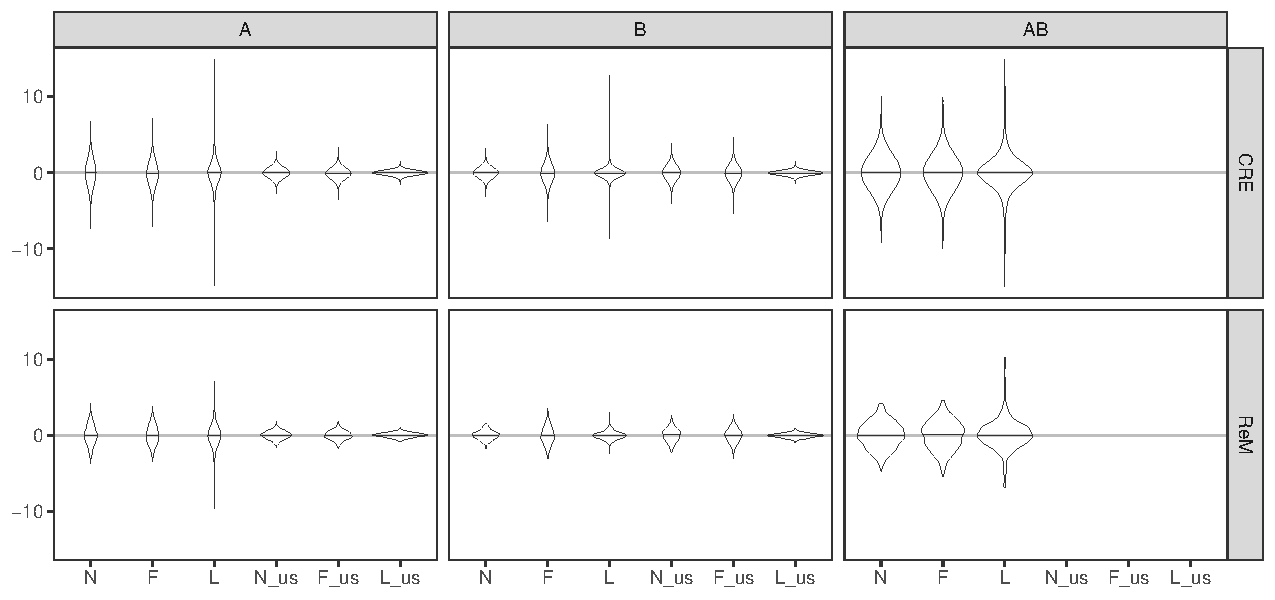
\includegraphics[width= \textwidth]{main_sep_factor_Q4_1eq2_N100_J20_diffb_22_23_24_31_nRep1e+05.pdf}
(a) $(\beta_{\mmm\pp}, \beta_{\pp\mmm}, \beta_{\pp\pp})  = (1_J, 0_J, -1_J)$ such that the $\gamma_q$'s differ considerably.
\end{center}


 \begin{center}
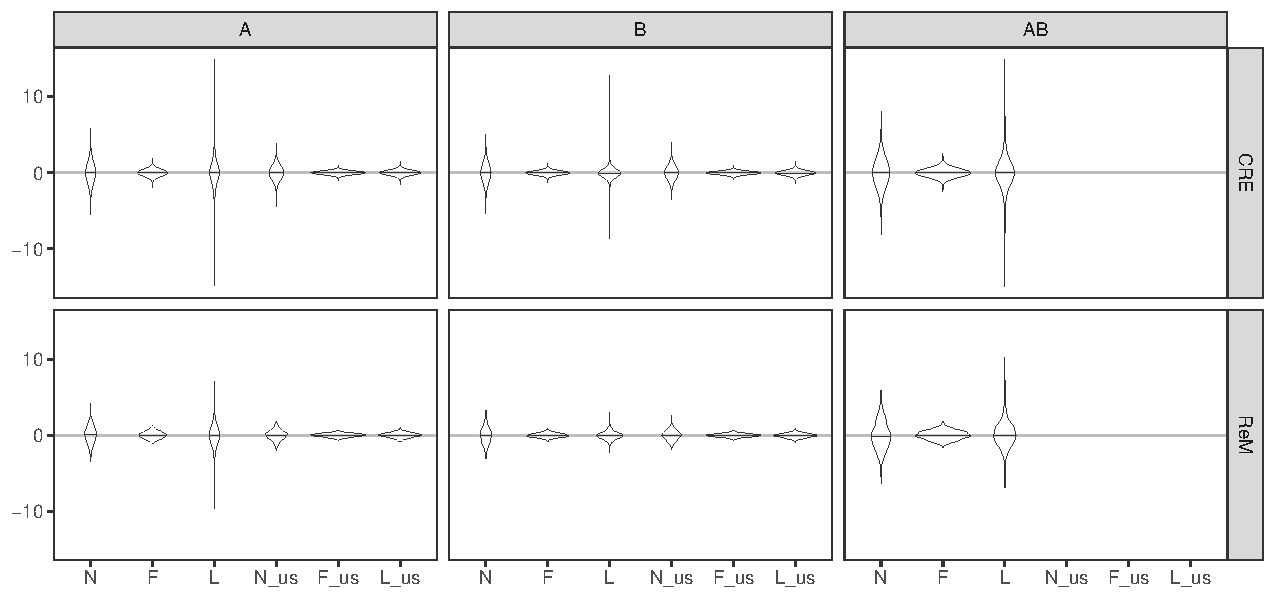
\includegraphics[width= \textwidth]{main_sep_factor_Q4_1eq2_N100_J20_sameb_22_23_24_31_nRep1e+05.pdf}
(b) $\beta_{\mmm\pp}=\beta_{\pp\mmm}= \beta_{\pp\pp} = 1_J$ such that the $\gamma_q$'s are fairly close.
\end{center}

\caption{\label{fig} Distributions of the differences between 2 times the \olss coefficients of $(A_i, B_i, A_iB_i)$ and the true values of $(\ta, \tb 	, \tab)$ over $100,000$ independent initial complete randomizations. CRE and ReM stand for results under complete randomization and rerandomization, respectively.}
\end{figure}

\section{Discussion}
Based on the asymptotic analysis and simulation, we recommend using restricted least squares on the fully interacted regression  for covariate adjustment in \mess when the sample size is  moderate relative to the number of covariates or treatment levels. 
%
Assume the restriction on the {\apo} is correctly specified and separate from that on the {\cpoc}. 
The resulting inference is consistent for estimating the finite-population average treatment effects regardless of whether the restriction on the correlations is correctly specified or not, and ensures additional efficiency over the \olss counterpart 
if the restriction on the correlations is indeed correctly specified under constant treatment effects. 
Simulation studies further show that it can have better finite-sample performance than the \olss counterpart even when the restriction is moderately misspecified.  

When prior knowledge on the {\apo} is less reliable, we recommend imposing restriction on only the correlations. The resulting estimator ensures consistency, yet can be at most as efficient as the \olss counterpart asymptotically. 
Importantly, all results are design-based, and hold without assuming any stochastic models for the potential outcomes.



%%%%%%%%%%%%%%%%%%%%%%%%%%%%%%%%%%%%%%%%%%%%%%
%% Funding information, if any,             %%
%% should be provided in the                %%
%% funding section.                         %%
%%%%%%%%%%%%%%%%%%%%%%%%%%%%%%%%%%%%%%%%%%%%%%


 

\bibliographystyle{plainnat}
\bibliography{refs_factorial-X}




\newpage
\setcounter{equation}{0}
\setcounter{section}{0}
\setcounter{figure}{0}
\setcounter{example}{0}
\setcounter{proposition}{0}
\setcounter{corollary}{0}
\setcounter{theorem}{0}
\setcounter{table}{0}
\setcounter{condition}{0}
\setcounter{lemma}{0}
\setcounter{remark}{0}



\renewcommand {\theproposition} {S\arabic{proposition}}
\renewcommand {\theexample} {S\arabic{example}}
\renewcommand {\thefigure} {S\arabic{figure}}
\renewcommand {\thetable} {S\arabic{table}}
\renewcommand {\theequation} {S\arabic{equation}}
\renewcommand {\thelemma} {S\arabic{lemma}}
\renewcommand {\thesection} {S\arabic{section}}
\renewcommand {\thetheorem} {S\arabic{theorem}}
\renewcommand {\thecorollary} {S\arabic{corollary}}
\renewcommand {\thecondition} {S\arabic{condition}}
\renewcommand {\thepage} {S\arabic{page}}
\renewcommand {\theremark} {S\arabic{remark}}


\setcounter{page}{1}

  \setcounter{equation}{0}
\renewcommand {\theequation} {S\arabic{equation}}
  \setcounter{lemma}{0}
\renewcommand {\thelemma} {S\arabic{lemma}}
   \setcounter{definition}{0}
\renewcommand {\thedefinition} {S\arabic{definition}}
   \setcounter{example}{0}
\renewcommand {\theexample} {S\arabic{example}}
   \setcounter{proposition}{0}
\renewcommand {\theproposition} {S\arabic{proposition}}
   \setcounter{corollary}{0}
\renewcommand {\thecorollary} {S\arabic{corollary}}

 

\begin{center}
\bf \Large 
Supplementary Material  to ``Covariate adjustment in multi-armed, possibly factorial experiments''
\end{center}

Sections \ref{sec:rem}--\ref{sec:2k_app} give  the additional results that complement the main text. 

Section \ref{sec:yb_app} gives the proofs of the results for $\hyba$ under complete randomization and rerandomization.

Section \ref{sec:ols_app} gives the proofs of the results on treatment-based regressions. 

Section \ref{sec:factor_proof} gives the proofs of the results on factor-based regressions. 

\section*{Notation}
Assume centered covariates with $\bar x=0_J$ throughout the {\sm} to simplify the presentation. 
For notational simplicity, we will use $ \hy$ and $\hyn$ interchangeably to denote the vector of $(\hy(1), \ldots, \hy(Q))^\T$ when no confusion would arise. 
Let $\sxyq =  (N-1)^{-1} \sumn  \cxi \{Y_i(q)-\by(q)\}$ with $\gamma_q  = \sxxinv S_{xY(q)}$. 
% Let $\hx(q) = N_q^{-1}\sumiq x_i$ be the sample means of $x_i$'s, concatenated as $\hat x = (\hx(1)^\T, \ldots, \hx(Q)^\T)^\T$. 

For a sequence of random vectors $(A_N)_{N=1}^\infty$ that converges in distribution to $A$,
let $\ei(A_N) = E(A)$ and $\covi(A_N) = \cov(A)$ denote the expectation  and covariance  with respect to the asymptotic distribution.
For two sequences of random vectors $\{A_N\}_{N=1}^\infty$ and $\{B_N\}_{N=1}^\infty$, 
we say $A_N$ and $B_N$ are asymptotically equivalent if $\sqrtn (A_N -  B_N) = \op$, denoted by $A_N \approxi B_N$. 
For two estimators $\hth_1$ and $\hth_2$ that are both consistent for some parameter $\theta \in \mrm$, $\hth_1 \approxi \hth_2$ implies that $\sqrtn (\hth_1 - \theta) \asim \sqrtn (\hth_2 - \theta)$ by Slutsky's theorem.

Let $\circ$ denote the Hadamard product of matrices. 
Then $
\vbi =  \core \circ S_{b,\infty}$ for $b\in\mb$, with $V_* =  \diag( S _{*,qq} /\pq )_{q\in\mt} -  S_* = \core \circ S_*$ as special cases for $\nfl$.
%For a set of real numbers, vectors, or matrices $\{u_q: q \in \mt\}$, let  $\diag(u_q)_{q\in\mt}$ denote the diagonal or block-diagonal matrix  with $u_q$'s on the diagonal. 
For random variables $A$ and $B$, let $$\proj(A \mid  1, B) = E(A) + \cov(A, B)\{\cov(B)\}^{-1}\{B-E(B)\}$$  be the linear projection of $A$ onto $(1, B)$, % with regard to the complete randomization, 
with residual  $\res(A \mid  1,B) = A - \proj(A \mid  1,B)$.
% [---the notation of proj and res is only used for one proof and hence quite ``local''. Worth defining it globally here?---]  }

\section{Rerandomization in the design stage}\label{sec:rem}
\subsection{Overview}

Rerandomization discards randomizations that do not satisfy a prespecified covariate balance criterion in the design stage of experiments \citep{cox:1982, morgan2012rerandomization}, and provides an alternative way to incorporate covariate data for additional efficiency.
A special type of rerandomization, ReM, uses the \mhld of $\htx = \hx(1) - \hx(0)$, denoted by $\|\htx\|_\mm = \htx^\T \{\cov(\htx)\}^{-1} \htx$, as the balance criterion under the treatment-control experiment, and accepts a randomization if and only if $\|\htx\|_\mm \leq a$ for some prespecified threshold $a$  \citep{morgan2012rerandomization, LD2018, LD20, ZDfrt}. 
\citet{branson} and \citet{AOS} extended their discussion to $2^K$ factorial experiments, yet did not consider regression adjustment in the analysis stage. 



We further the literature by providing a unified theory for ReM and regression adjustment in \mes. 
Specifically, we quantify the impact of ReM on the asymptotic efficiency of $\htl$ and $\htr$, respectively, with $\hts \ (\nf)$ being special cases of $\htr$. The results are coherent with the existing theory under the treatment-control experiment \citep{LD20}:
ReM has no effect on $\htl$ asymptotically, yet improves the asymptotic efficiency of $\htlr$ when the restriction on the correlations between potential outcomes and covariates is misspecified and separate from that on the average potential outcomes. 
The resulting estimator, though still not as efficient as $\htl$ asymptotically, can have better finite-sample performance when the sample size is moderate relative to the number of covariates or treatments.
This illustrates the duality between ReM and regression adjustment for improving efficiency under \mes, and %allows us to 
further expands the theoretical guarantees by $\htr$. 
The combination of ReM and $\htr$, in addition to delivering all guarantees as under complete randomization, further reduces the loss in asymptotic efficiency when the restriction is misspecified. 
It is thus our recommendation for covariate adjustment in \mess when $\htl$ is not practical.





\subsection{ReM under \mes}
ReM under the treatment-control experiment measures covariate balance by the \mhld of $\htx$. 
The presence of multiple treatment arms permits more flexible measures of  covariate balance.
Specifically, denote by $\hx = (\hx^\T(1) , \dots, \hx^\T(Q) )^\T$ the vectorization of covariate means $\hx(q) = \meaniq x_i$ over $q \in\mt$. 
For a prespecified $Q\times 1$ contrast vector $g = (g_1, \dots, g_Q)^\T$,  
\begina
\hd_g = \sumq  g_q \hx  (q) = ( g^\T \otimes \mI_J) \hx
\enda defines an intuitive measure of covariate balance across the $Q$ treatment arms, and includes $\htx$ as  a special case with $Q = 2$ and $g = (-1, 1)^\T$. 
Assume $H \geq 1$ of such measures are of interest, 
concatenated as 
\begina
\hd=(  \hd_{g_1}^\T, \dots, \hd_{g_H}^\T )^\T
= ( G\otimes  I_J)\hx, %\qquad \text{where} \ \ G =  ( g_1,  \dots,   g_H)^\T,
\enda 
where $G =  ( g_1,  \dots,   g_H)^\T$ for some prespecified, linearly independent $ g_h$'s.  
We can conduct ReM based on the \mhl distance of $\hd$, with the formal definition given in Definition \ref{def::rem-factorial} below. % and introduce the formal definition below.

\begin{definition}
[ReM]\label{def::rem-factorial} 
Draw an initial treatment allocation by the complete randomization in Definition \ref{def::complete-randomization}, and accept it  if and only if the resulting $\hd$ satisfies $\|\hd\|_\mm     \leq a$ for some prespecified threshold $a$. 
%$
%\mathcal{A} = \{   \|\hd\|_\mm     \leq a  \}
%$ 
%holds for some prespecified threshold $a$. 
%Draw a treatment vector from Definition \ref{def::complete-randomization} and accept it  if and only if the event
%$
%\mathcal{A} = \{   \|\hd\|_\mm     \leq a  \}
%$ 
%holds for some prespecified threshold $a$. 
\end{definition}


Complete randomization is a special case with $a = \infty$. 
The linear independence of $g_h$'s limits the maximum number of contrast vectors  to $H \leq Q-1$.
In the treatment-control experiment, this implies that there can only be one contrast vector, proportional to $g=(-1,1)^\T$. The resulting $\hd$ is proportional to $\htx$, illustrating the uniqueness of balance criterion when $Q=2$. 
In the $2^K$ factorial experiment, \citet{branson} and \citet{AOS} considered $G = \cs$, with $H = Q-1$ contrasts as those that define the $Q-1$ standard factorial effects. 
Experimenters in reality may choose $G$ that is very different from $\cs$, with $H \ll Q$ when $Q$ is large.
An intuitive choice is  $G = (c_{\{1\}}, \ldots, c_{\{K\}})^\T$, corresponding to the contrast vectors that define the $K$ main effects.  
This suggests the practical relevance of developing the theory of ReM in terms of general $G$.    




Recall the definition of $\hyba\in \my$ from \eqref{eq:my}, with $\hyba\asim \hyl$ if $\plim b = \gamma$. Theorem \ref{thm:rem_g} below clarifies the utility of ReM for improving the asymptotic efficiency of suboptimally adjusted $\hyba$ with $\plim b \neq \gamma$. 
Recall that 
\begine[(i)]
\item $\hys = \hybs \in\my$ for $\nfl$ from the comments after \eqref{eq:my}, 
\item  $\hyr  = \hybr  \in\my$ under \rlss subject to \eqref{eq:rest_noy} by Proposition  \ref{prop:noy}, and 
\item $\hyr  - \by = U \{\hybr  - \by\}$ with $\hybr  \in\my$ under \rlss subject to \eqref{eq:rest_sep} when $\rhy \neq 0$ and $\rhy\by =r_Y$ is  correctly specified by Proposition \ref{prop:sep}.
\ende
The result of Theorem \ref{thm:rem_g} hence implies the impact of ReM on $\hts  \ ( \nfl)$ and $\htr$ as direct consequences. 

Denote by $(\hyba\mid \ma)$, where $\ma = \{\remd\}$, the sampling distribution of $\hyba$ under {\rem}. 
Asymptotically, it is a convolution of  two independent  Normal and truncated Normal random vectors. The explicit form is not central to the discussion below and thus relegated to Theorem \ref{thm:rem_g_supp} in Section \ref{sec:rem_g}. 
 





\begin{theorem}\label{thm:rem_g}
{\prerem}
For $\hyba\in \my$ with $\plim b = \bi$, we have 
\begina
 \hyl \ \asim \ (\hyl \mid \ma) \ \succi \ (\hyba\mid \ma)  \ \succi\  \hyba
\enda
with $(\hyba\mid \ma) \asim \hyba\asim \hyl$ if $\bi = \gamma$.
\end{theorem}



Recall that $\plim \hbr = \gamma$ when the restriction on $\gamma$ is correctly specified and separate from that on $\by$. 
ReM thus has no effect on the asymptotic distribution of $\hyl$, or $\hyr$ when the restriction on $\gamma$ is correctly specified, but improves the asymptotic efficiency of $\hyr$ if $\rhg\gamma = r_\gamma$ is misspecified under separable restriction.
Inference based on $\hyl$ under ReM can therefore use the same Normal approximation as under complete randomization; likewise for that based on $\hyr$ when the restriction on $\gamma$ is correctly specified.
The same Normal approximation, however, will necessarily be over-conservative when $\rhg\gamma = r_\gamma$ is misspecified, highlighting the need of ReM-specific inference for better calibration. 
We relegate the details to Section \ref{sec:rem_plugin}.

In addition to the efficiency boost for the suboptimally adjusted $\hyba$'s, ReM also improves the coherence between estimators based on different regression adjustments. 
Let $\ei(\cdot\mid \ma)$ denote the asymptotic expectation under ReM.
\begin{corollary}\label{cor:close}
{\prerem} Then 
\begina
 \ei \big( \|\hyba - \hy\la b' \ra \|_2^2  \mid  \ma \big ) 
\ = \  \nu_{JH,a}   \ei\big( \|\hyba - \hy\la b' \ra \|_2^2  \big) 
\    \leq \     \ei \big( \|\hyba - \hy\la b' \ra \|_2^2\big)
\enda
  with $ \nu_{JH, a} =  P(\chi^2_{JH+2}< a)/P(\chi^2_{JH}< a) < 1$ for $b \neq b' \in \mb$.  
\end{corollary}


The $\hyba$ in Corollary \ref{cor:close} includes $\hys \ (\nfl)$ as special cases, and ensures that the discrepancy between the unadjusted and adjusted estimators is smaller under ReM than under complete randomization. This is a desirable property in empirical research. 


\section{Additional results on $\hyba\in \my$}\label{sec:yb_app_add_res}
We give in this section some additional results on the covariate-adjusted estimator $\hyba\in \my$ under {\cre} and {\rem}, respectively.
Assume throughout that $b = (b_1^\T, \dots, b_Q^\T)^\T \in\mb$ with $b_q \in \bbr^J$ and $\plim b = \bi = (b^\T_{1,\infty}, \ldots, b^\T_{Q, \infty})^\T$. % with $b_{q, \infty} = \plim b_q$.
Recall
\begina
\hyg = (\hy(1;\gamma_1), \ldots, \hy(Q; \gamma_Q))^\T
\enda as the oracle estimator defined by $\gq =(\gamma_1^\T,\dots, \gamma_Q^\T)^\T$.
Let 
$\db   = \diag\{(b_q - \gamma_q)^\T\}_{q\in\mt}$ with  
\begina
\hyba= \hy - \{\diag(b_q^\T)_{q\in\mt}\} \hx =  \hyg - \db   \hx,  
\enda 
where $\hat x = (\hx(1)^\T, \ldots, \hx(Q)^\T)^\T$. 
Let  
$\dbi  = \plim D_b  = \diag\{(b_{q,\infty} - \gamma_q)^\T\}_{q\in\mt}$. 

\subsection{Sampling properties under complete randomization}
\begin{lemma}\label{lem:yg}
Assume {\cre}. Then 
\begina
E\{\hyg\} = \by, \qquad \cov\{\hyg\} =  N^{-1}V_\lin, \qquad \cov\{\hyg ,\hx\}= 0.
\enda
Further assume Condition \ref{asym}. Then 
\begina
\sqrtn \beginp
\hyg - \by\\
\hx
\endp \rs \mn\left\{ 0 , \beginp V_\lin & 0   \\ 0   & V_x \endp \right\},
\enda
where $V_x = N\cov(\hx) =  \core  \otimes  \sxx$. 
\end{lemma}

Lemma \ref{lem:yg} and Lemma \ref{lem:yb} together  ensure that $\hyg \asim \hyl \succi \hyba$ for all $\hyba\in\my$. 
This justifies $\hyg$ as the oracle estimator with fixed adjustment coefficients $b_q = \gamma_q \ (\qit)$, extending \citet[][Example 9]{LD20} to \mes. 
Theorem \ref{thm:optimal_gamma} below states a stronger result than Lemma \ref{lem:yb}, characterizing the asymptotic distance of $\hyba\in \my$ from the oracle.



\begin{theorem}\label{thm:optimal_gamma} 
{\precre}
For $\hyba\in \my$ with $\plim b = \bi$, we have
\begina
\hyba &\approxi &\hyg - \dbi   \hx  \ \preci \  \hyg
\enda with  $\vbi = N\covi\{\hyba\} = V_\lin + \dbi V_x \dbi^\T$. In particular, $\hyba \approxi \hyg$  if $\dbi V_x \dbi^\T = 0$. A sufficient condition for this is $\bi = \gamma$.  
\end{theorem}

Theorem \ref{thm:optimal_gamma} states the asymptotic equivalence of $\hyba$ and $\hyg -\dbi \hx = \hybi$, suggesting $\dbi\hx$ as the distance of $\hyba$ from the optimally adjusted $\hyg$.
Recall that  $\gamma_q$ gives the target parameter of $\wiq x_i$ in \eqref{eq:lm_l} from the derived linear model perspective.  The additive and fully interacted regressions can thus also be viewed as two ways to estimate the optimal adjustment coefficients $\gamma_q \ (q\in\mt)$. 
In particular, we can estimate $\gamma_q$ by the \olss coefficient of $\wiq x_i$, namely $\hb_{\lin,q}$, from the fully interacted regression \eqref{eq:lm_l}, and by the \olss coefficient of $x_i$, namely $\hbf$, from the additive regression \eqref{eq:lm_f}. 
%
 Let $ b_\fisher = 1_Q  \otimes \hbf $ and $ b_\lin=  (\hb_{\lin,1}^\T, \dots, \hb_{\lin,Q}^\T)^\T = \hbl$ be the resulting estimators of the full vector $\gamma$. 
Proposition \ref{prop:numeric_corr} below
establishes the numeric identity between $\hys$ and $\hybs $ for $\fl$. 

\begin{proposition}\label{prop:numeric_corr}
$\hy_* = \hybs $ for $\ms$ with $b_\neyman = 0_{JQ}$, $b_\fisher = 1_Q\otimes \hbf$, and $b_\lin = \hbl$.  
%
Further assume \creasym. Then 
$\hbf = \gp + \op$ and $\hbl = \bg + \op$ with $ \plim b_\fisher =  1_Q\otimes \gp$ and $\plim b_\lin =\gamma$. 
\end{proposition}

As a result, $b_\lin$ is consistent for $\gamma$, whereas
$b_\fisher$ in general is not. 
By Theorem \ref{thm:optimal_gamma}, the asymptotic efficiency of $\hyl$ over $\my$ in Lemma \ref{lem:yb} is essentially the consequence of its asymptotic equivalence with $\hyg$ given $b_\lin = \gamma + \op$.
The equal correlation condition, on the other hand, ensures $b_\fisher = \gamma + \op$ such that $\hyf  \approxi \hyl\approxi \hyg$.
This gives the intuition behind Lemma \ref{lem:reg}.  The asymptotic equivalence between $\hb_{\lin,q}$ and $\gamma_q$ is no coincidence but the consequence of the fully interacted regression being numerically equivalent to fitting $Q$ treatment-specific regressions: $Y_i \sim 1+x_i$ over $\{i: Z_i = q\}$. This ensures that $\hb_{\lin,q}$ equals the coefficient vector of $x_i$ in the $q$th regression, and converges in probability to $\gamma_q$ as its population analog.


\subsection{Sampling properties under ReM}\label{sec:rem_g}


Let  
\beginy\label{eq:vb}
\vpbi = \dbi  (\Phi\otimes \sxx)\dbi  ^\T, \qquad \vrbi= \vbi  - \vpbi
\endy with  $\Phi  =  \einv   G^\T ( G \einv    G^\T)^{-1}  G \einv$.
Following \cite{AOS}, let $(\vpbi)^{1/2}_{JH}$ denote a $Q\times JH$ matrix that satisfies $(\vpbi)^{1/2}_{JH} \{(\vpbi)^{1/2}_{JH}\}^\T = \vpbi$. 
Let $\epsilon \sim \mn(0_Q, I_Q)$ and $\ml \sim \ep' \mid  (\| \ep'\|_2^2 \leq a)$ be two independent standard and truncated Normal random vectors with  $\ep' \sim \mn(0_{JH}, I_{JH})$.
Then $\ml \succeq \ep'$ with mean  $0_{JH}$ and covariance $\nu_{JH, a}  I_{JH}< I_{JH}$.  Theorem \ref{thm:rem_g_supp} below states the asymptotic distribution of $\hyba$ under ReM.

\begin{theorem}\label{thm:rem_g_supp}
{\prerem} 
For $\hyba\in \my$ with $\plim b = \bi$, we have
\beginy\label{eq:rem_dist}
\big\{ \sqrtn (\hyba-\bar Y) \mid \ma\big\}  & \asim &   (\vrbi)^{1/2} \cdot  \epsilon +  (\vpbi)^{1/2}_{JH} \cdot   \mL
\endy
with 
\begina
 V_\lin^{1/2} \cdot \epsilon \ \ \succeq \ \  (\vrbi)^{1/2} \cdot  \epsilon +  (\vpbi)^{1/2}_{JH} \cdot   \mL \ \  \succeq \ \ \vbi^{1/2}\cdot \epsilon. 
\enda
In particular,  
\begina
\{ \sqrtn (\hyba-\bar Y) \mid \ma\} \  \ \asim\ \ V_\lin^{1/2} \cdot \ep \  \ \sim  \ \ \mn(0_Q, \vl)
\enda if and only if $\dbi  (\Phi\otimes \sxx)\dbi  ^\T = 0$. A sufficient condition for this is $\bi = \gamma$. 
\end{theorem}

Recall that $\sqrtn(\hyl - \by) \asim V_\lin^{1/2}\cdot \epsilon$ and $\sqrtn(\hyba- \by) \asim V_{b,\infty}^{1/2} \cdot \epsilon$ by Lemma \ref{lem:yb}. 
Theorem \ref{thm:rem_g_supp} implies Theorem \ref{thm:rem_g} as a direct consequence, and clarifies the asymptotic relative efficiency between $(\hyba\mid \ma)$, $\hyba$, and $\hyl$. 
The choice of $(\vpbi)^{1/2}_{JH}$ is not unique, but the asymptotic distribution is.

In addition, recall that $\hyba\approxi  \hyg - \dbi  \hx $, with $\hyg$ being asymptotically independent of $\hx$. 
ReM based on $\hd = (G\otimes I_J)\hx$ thus affects only the $\dbi\hx$ part asymptotically, and increases its peakedness if $\bi \neq \gamma$. 
%
This affords the intuition for the asymptotic distribution of $\hyba$ being a convolution of independent Normal and truncated Normal when $\dbi \neq 0$, and ensures that the asymptotic sampling distribution of $\hyl = \hy\la b_\lin\ra$ remains unchanged under  ReM given $\plim b_\lin = \gamma$.  

A key distinction from the treatment-control experiment is that choosing a small $a$ alone no longer suffices to ensure that $\hyba$ is asymptotically almost as efficient as $\hyl$ when $\bi \neq \gamma$ \citep{LD2018}.
In particular, a small $a$ ensures $N\covi\{\hyba\} \approx \vrbi$, with 
 $\vrbi  - \Vl = \dbi \{(\einv -\po - \Phi)\otimes \sxx\} \dbi^\T \geq 0$.
To have $\vrbi = \Vl$ thus entails additional conditions. % to ensure  $\dbi   \{(\einv -\po - \Phi )\otimes \sxx\} \dbi^\T = 0$. 
Without further assumptions on  $\bi$,  this requires $\einv -\po - \Phi =0$, with a sufficient condition given by $H=Q-1$; see Lemma \ref{lem:gimmick}. 
ReM under the treatment-control experiment is a special case with $H = 1 = Q-1$.


\subsection{ReM-specific inference based on  plug-in distributions}\label{sec:rem_plugin}
Recall that ReM increases the peakedness of $\hyr$ when the restriction on $\gamma$ is misspecified. 
The usual Normal approximation will therefore be over-conservative, deterring statistically significant findings. We consider below inference based on ReM-specific sampling distributions to avoid this issue. 

Recall from \eqref{eq:rem_dist} the asymptotic distribution of $\hyba$ under ReM.  
With $\ep$ and $\ml$ both following known distributions, the only parts that are unknown are $\vrbi$ and $\vpbi$. 
We can estimate them using their respective sample analogs, denoted by $\hvrbi$ and $\hvpbi$, respectively, and then conduct ReM-specific inference based on the distribution of 
\beginy\label{eq:plugin}
(\hvrbi)^{1/2} \cdot  \epsilon +  (\hvpbi)^{1/2}_{JH} \cdot   \mL.
\endy

In particular, recall that $\hblq$ %as the coefficient vector of $\wiq x_i$ from the \olss fit of \eqref{eq:lm_l}.  The properties of \olss ensure that $\hblq$ 
equals the coefficient vector of $x_i$ from the \olss fit of  $Y_i \sim 1+ x_i$ over $\{i:Z_i = q\}$, and hence gives an intuitive estimator of $\gamma_q$.
Let 
\begina
\hat S_{b, \infty, qq}  = (N_q-1)^{-1}\sumiq \left[Y_i - b_{q}^\T x_i - \{\hy(q) - b_{q}^\T \hx(q)\} \right]^2, \qquad \hat V_{b,\infty} = \diag(\hat S_{b, \infty,qq}/e_q)_\qit 
\enda
be estimators of $S_{b,\infty,qq}$ and $\vbi$, respectively. 
Then 
\begina
\hvpbi = \hat D_{b,\infty}(\Phi\otimes \sxx)  \hat D^\T_{b,\infty}, \qquad \hvrbi = \hat V_{b,\infty} - \hvpbi,
\enda 
where $  \hat D_{b,\infty} = \diag\{(b_q - \hblq)^\T\}_{\qit}$. 

Proposition \ref{prop:inference} below follows from \citet[][Lemma A10]{LD2018}, and ensures the asymptotic validity of the inference based on \eqref{eq:plugin}. 

\begin{proposition}\label{prop:inference}
{\prerem}
Then 
\begina
\hvpbi = \vpbi + \op, \qquad \hvrbi  = \vrbi + S_{b,\infty} + \op. 
\enda 
\end{proposition}

For $\hys = \hybs  \ (\nf)$ as direct outputs from \olss fits, 
we can also estimate $\vbi = V_*$ by $N\hat\Psi_*$, which is asymptotically equivalent to the $\hat V_{b,\infty}$ defined above.


\section{Additional results on RLS}\label{sec:rls_app_res} 
\subsection{Properties under general restriction}
Recall that $\mr=  \ccinvl R^\T\{R \ccinvl R^\T\}^{-1}$ from Lemma \ref{lem:hthr}. 
Let $\mri = \plim \mr$ be the finite probability limit of $\mr$ under complete randomization and Condition \ref{asym}; see \eqref{eq:mri} for the explicit form. 

Let $\xir$ be the first $Q$ rows of $- \mr\reslp $. 
Let $\sri$ be the upper-left $Q\times Q$ submatrix of $(I_p - \mri R) {\{N \covi(\hth_\lin)\}} (I_p - \mri R)^\T$; we give the explicit form of $N \covi(\hth_\lin)$ in   Lemma \ref{lem:hth}.


Recall that $\emat = \diag(e_q)_{q\in\mt}$ with $e_q = N_q/N$. 
Let 
\begina
\dz  = [R \ \diag\{\einv, \esinv\} R^\T]^{-1}.
\enda 
Write $R = (\ry, \rg)$, with $\ry$ and $\rg$ denoting the columns of $R$ corresponding to $\by$ and $\gamma$, respectively. 
Theorem \ref{thm:rls_g} below quantifies the asymptotic behaviors of $\hyr $ for general $R$, and suggests that $\hyr $ is in general not consistent for $\by$ unless $\ry = 0$ or \eqref{eq:restriction} is correctly specified. 


\begin{theorem}\label{thm:rls_g}
Assume \rlss subject to \eqref{eq:restriction}. Then 
\begina
\hyr  = \hybr  -  \einv \ryt  [ R \{N\ccinvl\} R^\T ]^{-1}(R\hthl-r),
\enda where $\hbr \in \mb$ with $\plim\hbr = \gamma -   (\es )^{-1} \rgt \dz  (R\tl  - r) $. 
Further assume \creasym. Then 
\begina
\hyr  - \by  -  \xir =  \op, \qquad \sqrtn(\hyr   -\by - \xir ) \rs  \mn(0_{Q}, \sri)
\enda
with 
\begine[(i)]
\item $ \xir=  - \einv  \ryt  \dz(R\tl  -r)+\op$;
\item $\xir = 0$, and hence   $\sqrtn(\hyr  -\by) \rs  \mn(0_{Q}, \sri)$, if \eqref{eq:restriction} is correctly specified.  
\ende
\end{theorem}

Theorem \ref{thm:rls_g} implies $\plim \xir = - \einv  \ryt  \dz(R\tl  -r)$ as the asymptotic bias of $\hyr$. Juxtapose Theorem \ref{thm:rls_g} with Theorems \ref{thm:noy} and \ref{thm:sep} in the main text. 
The consistency of $\hyr$ in general requires the whole restriction \eqref{eq:restriction} to be correctly specified,  whereas 
special structures like $R_Y = 0$ or $R = \diag(\rhy, \rhg)$ promise weaker sufficient conditions.
In particular, the {\go} restriction ensures consistency regardless of whether the restriction on $\gamma$ is correctly specified or not; likewise for the {\sr}  to ensure consistency as long as the restriction on $\by$ is correctly specified. 


\subsection{Asymptotic Normality under {\sr}}

Theorem \ref{thm:sep_app} below complements Theorem \ref{thm:sep} in the main paper, and gives the asymptotic distribution of $\hyr$ when $\rhy\by = r_Y$ is misspecified. Recall that $U =I_Q - \einv \rhy^\T   (\rhy \einv \rhyt)^{-1} \rhy$ and $\mur =- \einv \rhy^\T   (\rhy \einv \rhyt)^{-1} (\rhy\by - r_Y)$ for $\rhy \neq 0$. 


\begin{theorem}\label{thm:sep_app}
Assume {\cre}, Condition \ref{asym}, and \rlss subject to \eqref{eq:rest_sep} with $\rhy \neq 0$. Then 
%$
%\hyr   = U \hybr  + \einv \rhy^\T   (\rhy \einv \rhyt)^{-1}r_Y
%$ 
%with  
%$$
%\hyr  - \by -\mur = U\{\hybr  - \by\}.$$
%Further assume  \creasym. 
%Then 
$$
\sqrt N(\hyr  - \by -\mur) \rs \mathcal N(0_Q, U  \vlr  U^\T),
$$
where 
\begine[(i)]
\item $\mur = 0$ if $\rhy\by=r_Y$ is correctly specified; 
\item $\vlr \geq \vl$, and satisfies $\vlr = \vl$ if $\rho_\gamma \gamma = r_\gamma$ is correctly specified.
\ende
\end{theorem}

Echoing the comments after Theorem \ref{thm:gm}, the restrictions on $\by$ and $\gamma$ affect the asymptotic bias and variance, respectively. 


 
\subsection{Numeric properties of RLS}

We present in this subsection some useful numeric properties about \rls. 
The results are stated in terms of general regression formulation to highlight their generality.
 
For an $N \times 1$ vector $ Y$  and an $N\times p$ matrix $X$, consider the \rlss fit of 
\begina
Y = X \hat\beta + \hep \qquad \text{subject to} \ \ R\hat\beta = r,
\enda
where $\hb$ and $\hep = (\hep_1, \ldots, \hep_N)^\T$ denote the \rlss coefficient vector and residuals, respectively. 
To simplify the presentation, we suppress the subscript ``$\rr$'' for \rlss in this subsection when no confusion would arise.
We propose to estimate the sampling covariance of $\hb$ by
\beginy\label{eq:ehw_rls}
\hv = (I_p - \mr R) (X^\T X)^{-1} X^\T \big\{\diag(\hep^2_i)_{i=1}^N \big\} X (X^\T X)^{-1} (I_p - \mr R)^\T,
\endy
where $\mr =  (X^\T X)^{-1} R^\T\{R (X^\T X)^{-1} R^\T\}^{-1}$.
Refer to $\hv$ as the {\it robust covariance from \rls.} 





The following lemma states the invariance of \rlss to {\ndt}.

\begin{lemma}\label{lem:inv_rls} 
Consider an $N \times 1$ vector $ Y$  and two $N\times p$ matrices, $X$ and $X'$, that satisfy $X' = X\Gamma$ for some nonsingular $p\times p$ matrix $\Gamma$. 
The \rlss fits of 
\begina
\begin{array}{ll}
Y =  X\hbb+ \hep &\quad\text{subject to} \ \ R \hbb = r, 
 \\
Y =  X' \hbb' +\hep' &\quad \text{subject to} \ \ (R\Gamma) \hbb' = r
\end{array}
\enda
yield $(\hb, \hep, \hv)$ and $(\hb', \hep', \hv')$ as the coefficient vectors, residuals, and robust covariances by \eqref{eq:ehw_rls}, respectively. They
satisfy 
$$
\hbb = \Gamma\hbb',\qquad
\hep = \hep',\qquad
\hv = \Gamma \hv' \Gamma^\T.
$$ 
\end{lemma}

Lemma \ref{lem:ehw_g} below presents a novel result on the numeric equivalence between the robust covariance \eqref{eq:ehw_rls} from the \rlss fit and that from the \olss fit of a corresponding restricted specification.  
Importantly, whereas Lemma \ref{lem:inv_rls} allows for nonzero $r$, Lemma \ref{lem:ehw_g} requires that $r=0$. 





\begin{lemma}\label{lem:ehw_g}
Consider the \rlss fit of 
\beginy\label{eq:fs}
Y = X \hb + \hep\qquad \text{subject to} \ \ R\hb = 0,
\endy
where $X \in \mathbb R^{N\times p}$, $R \in \mathbb R^{l \times p}$, and $\hb \in \mathbb R^{p}$ and $\hep\in \mathbb R^N$ denote the \rlss coefficient vector and residuals, respectively.
Then 
\begine[(i)]
\item The corresponding restricted specification can be formed as 
\beginy\label{eq:rs}
Y = \big\{X\rpt(\rpp\rpt)^{-1}\big\}\hb_\ols + \hep_\ols,
\endy
where $ \rpp \in \mathbb R^{(p-l) \times p}$ is an orthogonal complement of $R$ in the sense that $(\rpt, R^\T)$ is nonsingular with $\rpp R^\T   = 0$.
Let $\hb_\ols\in  \mathbb{R}^{p-l}$ and $\hep_\ols \in  \mathbb{R}^N $ denote the coefficient vector and residuals from the \olss fit of \eqref{eq:rs}. 
Then 
\begina
\hb_\ols = \rpp \hb , \qquad \hep_\ols = \hep.
\enda 
\item Let $\hv_\rls = \rpp \hv \rpt$ denote the robust covariance of $\rpp \hb$ from the \rlss fit of \eqref{eq:fs} by \eqref{eq:ehw_rls}. 
Let $\hv_\ols$ denote the \ehws covariance of  $\hb_\ols$ from the \olss fit of \eqref{eq:rs}. Then 
\begina
\hv_\rls = \hv_\ols.
\enda 
\ende
\end{lemma}

Lemma \ref{lem:ehw_g} includes Examples \ref{ex:ehw_equiv} and \ref{ex:ehw_equiv_2} below as special cases, which correspond to the unadjusted and additive regressions, respectively. 

\begin{example}\label{ex:ehw_equiv}
For an $N \times 1$ vector $ Y$, an $N\times k$ matrix $ X_1$, and an $N\times l$ matrix $ X_2$, consider the \rlss fit of 
\begina
Y =  X_1 \hb_1 +  X_2 \hb_2 + \hep \qquad\text{subject to} \ \ \hb_2 = 0,
\enda
where $\hb_1$, $\hb_2$, and $\hep$ denote the \rlss coefficient vectors and residuals, respectively. 
Let 
$\hv_\rls$ denote the robust covariance of $\hb_1$ by \eqref{eq:ehw_rls}.
Alternatively, consider the \olss fit of 
\begina
Y =  X_1 \hb_{1,\ols}  + \hep_\ols 
\enda
as the corresponding restricted specification, 
where $\hb_{1,\ols}$ and $\hep_\ols$ denote the \olss coefficient vector and residuals, respectively. 
Let $\hv_\ols$ denote the \ehws covariance of $\hb_{1,\ols}$. 
Then 
\begina
\hb_1 = \hb_{1,\ols},\qquad \hep = \hep_\ols, \qquad
\hv_\rls = \hv_\ols.
\enda
\end{example}

\begin{example}\label{ex:ehw_equiv_2}
For an $N \times 1$ vector $ Y$, an $N\times k$ matrix $ X_0$, and $N\times l$ matrices $ X_1,\ldots, X_Q$, consider the \rlss fit of 
\begina
Y =  X_0 \hb_0 +  X_1 \hb_1 +\cdots + X_{Q} \hb_Q + \hep \qquad\text{subject to} \ \ \hb_1 = \cdots = \hb_Q,
\enda
where $\hb_q \ (q =\zt{Q})$ and $\hep$ denote the \rlss coefficient vectors and residuals, respectively. 
Let 
$\hv_\rls$ denote the robust covariance of $\hb_0$ by \eqref{eq:ehw_rls}. 
Alternatively, consider the \olss fit of 
\begina
Y =  X_0 \hb_{0,\ols}  + \xpp \hb_\ols + \hep_\ols 
\enda
as the corresponding restricted specification, where $\hb_{0,\ols}$, $\hb_\ols$, and $\hep_\ols$ denote the \olss coefficient vectors and residuals, respectively. Let $\hv_\ols$ denote the \ehws covariance of $\hb_{0,\ols}$.  
Then 
\begina
\hb_0 = \hb_{0,\ols},\qquad \hb_q = \hb_{\ols} \quad (q=\ot{Q}), \qquad \hep = \hep_\ols, \qquad
\hv_\rls = \hv_\ols.
\enda
\end{example}

Recall that $\hsis$ and $\hsrs$ denote the robust covariances of $\hys \ (\nf)$ from the \olss fits of \eqref{eq:lm_n}--\eqref{eq:lm_f} and the \rlss fits of \eqref{eq:lm_l}, respectively. The numeric equivalence between $\hsis$ and $\hsrs$ follows immediately from Examples \ref{ex:ehw_equiv} and \ref{ex:ehw_equiv_2}. 

\begin{proposition}\label{prop:ehw_equiv}
$\hsis = \hsrs$ for $\nf$.
\end{proposition}


\section{Additional results on $2^K$ factorial experiments}\label{sec:2k_app}

\subsection{Design-based theory for the general regression} \label{sec:2k_app_s}
For $\mfp \subseteq \pk$ and $\mfpp \subseteq \pk' = \{\emptyset\} \cup \pk$, consider 
\beginy\label{eq:lm_2k_g}
Y_i \sim 1 + \sum_{\mk \in \mfp} \zimks + \sum_{\mk \in \mfp'} \zimks \, \cxi, 
\endy 
where  $Z_{i, \emptyset}x_i = x_i$ with $Z_{i, \emptyset} = 1$ if $\mk = \emptyset \in \mfp'$. 
It is a general specification, and includes \eqref{eq:lm_2k_n}--\eqref{eq:lm_l_2k_u} as special cases with different choices of $(\mfp, \mfpp)$, summarized in Table \ref{tb:specs_2k_app}. 
The resulting regression is factor-saturated if $\mfp = \pk$, and factor-unsaturated if $\mfp \subsetneq \pk$ with $  \mfm  = \pk \backslash \mfp \neq \emptyset$.

\begin{table}[t]
\renewcommand{\arraystretch}{1.3}
\caption{\label{tb:specs_2k_app}  The choices of $(\mfp, \mfp')$ in \eqref{eq:lm_2k_g} for the six factor-based regressions in Table \ref{tb:specs_2k}.  
We use $\emptyset$ to denote the empty set, and use $\{\emptyset\}$ to denote the set that contains the empty set as the only element. }
\begin{center}
 
\begin{tabular}{|c|l|c|c|}\hline
  & & &\\
base model & \multicolumn{1}{c|}{regression equation} & $\mfp$ & $\mfp'$  \\\hline
%%%%%%%%%%%%%
&\eqref{eq:lm_2k_n}: $Y_i \sim 1 + \sum_{\mk \in \pk} \zimks$ &   & $\emptyset$      \\\cline{2-2}\cline{4-4}
%%%%%%%%%%%%%%%%%%%%%%%
$Y_i \sim 1 + \sum_{\mk \in \pk} \zimks$ &\eqref{eq:lm_2k_f}: $Y_i \sim 1 + \sum_{\mk \in \pk} \zimks+ \cxi $  & $\pk$ & $\{\emptyset\}$      \\\cline{2-2}\cline{4-4}
%%%%%%%%%%%%%%%%%%
(factor-saturated) &\eqref{eq:lm_2k_l}: $Y_i \sim 1 + \sum_{\mk \in \pk} \zimks + \cxi  + \sum_{\mk \in \pk} \zimks \cxi  $&   & $\pk'$  \\\hline
%%%%%%%%%%%%%%%%%%%%%%%
& \eqref{eq:lm_n_2k_u}: $Y_i \sim 1 + \sum_{\mk \in \mfp} \zimks$ &     & $\emptyset$  \\\cline{2-2}\cline{4-4}
%%%%%%%%%%%%%%%
{$Y_i \sim 1 + \sum_{\mk \in \mfp} \zimks$}&\eqref{eq:lm_f_2k_u}: $Y_i \sim 1 + \sum_{\mk \in \mfp} \zimks+\cxi $ & $\mfp$   & $\{\emptyset\}$  \\\cline{2-2}\cline{4-4}
%%%%%%%%%%%%%%%%%%%%%%%
(factor-unsaturated) & \eqref{eq:lm_l_2k_u}: $Y_i \sim 1 + \sum_{\mk \in \mfp} \zimks + \cxi  + \sum_{\mk \in \mfp} \zimks \cxi   $ &     & $\{\emptyset\} \cup \mfp$  \\\hline
\end{tabular}		

\end{center}
\end{table}


Assume that $\mfp$ is non-empty throughout this section. We state below the design-based properties of the \olss outputs from \eqref{eq:lm_2k_g}. The result includes those of   \eqref{eq:lm_2k_n}--\eqref{eq:lm_l_2k_u} as special cases. 


Let
\begina
\tsp   = \{\tsmk   : \mk \in \mfp \} = \csp\by, \qquad
\tsm = \{\tmk : \mk\in\mfm \} = \csm \by
\enda
concatenate the effects of interest and nuisance effects corresponding to $\mfp$ and $\mfm = \pk \backslash \mfp$, respectively.
To simplify the presentation, define $\csm = 0_J^\T$ if $\mfm$ is empty, with $\tsm = 0$. 

Let $\mfm' = \pk' \backslash\mfp'$, and let $\csm'$ concatenate rows of $\{\csmk:\mk\in \mfm'\}$, with $c_{\sss,\emptyset} = 2^{-(K-1)} 1_Q$ and $\csm' = 0_J^\T$ if $\mfm'$ is empty.


Let $\ttrmk$ be 2 times the coefficient of $\zimk$ from the \olss fit of  \eqref{eq:lm_2k_g}, vectorized as $$\ttrp  = \{\ttrmk: \mk\in\mfp\}.$$ 
Let $\torp $ be the \ehws covariance of $\ttrp$ from the same \olss fit. 

Let $\hyrs $ be the coefficient vector of $t_i$ from the \rolss fit of  \eqref{eq:lm_l} subject to 
\beginy\label{eq:rest_2k_g}
\csm \by = 0,\qquad (\csm' \otimes I_J) \gamma = 0. 
\endy 
In case where $\mfm = \emptyset$ such that $\csm = 0_J^\T$, then $\csm \by = 0$ is correctly specified by definition, implying no restriction on $\by$; likewise for the case with $\mfm' = \emptyset$ to imply no restriction on $\gamma$.
Let $\hat\Psi_{\rr,\sss}$ be the robust covariance of $\hyrs$ based on the definition in Section \ref{sec:ehw_rols}.


Proposition \ref{prop:2k_g} below states the numeric correspondence between $(\ttrp, \torp )$ and $(\hyrs, \hat\Psi_{\rr,\sss})$. 

\begin{proposition}\label{prop:2k_g}
$\ttrp   =  \csp\hyrs$ and $\torp  = \csp\hat\Psi_{\rr,\sss}\csp^\T$. 
\end{proposition}

 The one-to-one correspondence between $t_i = \{ 1(Z_i = q): q\in\mt\}$ and $\{1, \zimks: \mk\in\pk\}$ ensures that $2^{-1}\tmk$, $2^{-1}(c^\T_{\sss,\emptyset} \otimes I_J) \gamma$, and $2^{-1}(\cmk^\T\otimes I_J) \gamma$ give the target parameters of $\zimk$, $x_i$, and $\zimk x_i$ for $\mk \in \pk$ in \eqref{eq:lm_2k_l}, respectively, from the derived linear model perspective; see the proof of Proposition \ref{prop:2k_g} in Section \ref{sec:factor_proof}.
Regression \eqref{eq:lm_2k_g} can thus be seen as a restricted variant of \eqref{eq:lm_2k_l}, assuming \eqref{eq:rest_2k_g}.
This gives the intuition behind \eqref{eq:rest_2k_g} and the correspondence between $\ttrp$ and $\hyrs$.

The design-based properties of $\ttrp $  then follow from those of $\hyrs$ in  Lemma \ref{lem:yb} and Theorems \ref{thm:noy}--\ref{thm:gm}. 
Let $\hbrs$ and $\vrrs$ be the values of $\hbr$ and $\vrr$ associated with $\hyrs$. 
Then $\hbrs \in \mb$ with $\plim \hbrs = \gamma$ and $\vrrs = V_\lin$ if $(\csm' \otimes I_J) \gamma = 0$ by Propositions \ref{prop:noy} and \ref{prop:sep}.
Let 
\begina
\us =I_Q - \einv \csm^\T   (\csm \einv \csmt)^{-1} \csm, \qquad \murs =- \einv \csm^\T   (\csm \einv \csmt)^{-1} \tsm
\enda
%
%\begina
%\us =I_Q - \einv \csm^\T   (\csm \einv \csmt)^{-1} \csm, \qquad \murs =- \einv \csm^\T   (\csm \einv \csmt)^{-1} \tsm
%\enda
%
be the values of $U$ and $\mur$ at $\rhy = \csm$, respectively, if $\mfm  \neq \emptyset$.  
Recall $\ttsp = \{\ttsmk: \mk\in\mfp\}$ as the estimators of $\tsp$ from the factor-saturated regressions \eqref{eq:lm_2k_n}--\eqref{eq:lm_2k_l} with $\ttlp \succi \ttnp, \ttfp$. 

\begin{corollary}\label{cor:2k_g}
\begine[(i)]
\item For \eqref{eq:lm_2k_g} that is factor-saturated with $\mfp = \pk$, we have 
\begini
\itemc $\ttrp   =  \cs\hybrs $. 
\itemc $\sqrt N(\ttrp - \ts ) \rs \mn(0, \cs \vrrs \cs^\T)$ under \creasym,  with $\ttrp \preci \ttl$ and $\torp$  being asymptotically conservative for estimating the true sampling covariance. 
%
In particular, $\ttrp \asim \ttl$ if $(\csm' \otimes I_J) \gamma = 0$. A sufficient condition for this is Condition \ref{cond:equal} and \eqref{eq:lm_2k_g} includes $x_i$.
\endi 
%%%%%%%%%%%%%%%%
%%%%%%%%%%%%%%%%
\item For \eqref{eq:lm_2k_g} that is factor-unsaturated with  $\mfp  \subsetneq \pk$ and $\mfm  \neq \emptyset$, we have 
\begini
\itemc
$
\ttrp  - \tsp -\csp\murs = \csp\us\{\hybrs  - \by\}$, where $ \csp \murs = 0$ if $\tsm = 0$. 
\itemc $\sqrt N(\ttrp  - \tsp - \csp \murs) \rs \mathcal N(0, \csp \us  \vrrs  \us^\T \csp^\T)$  under \creasym, with $\torp$ being asymptotically conservative for estimating the true sampling covariance.

Further assume Condition \ref{cond:sa}. Then $\vrrs = V_\lin$ with $
\ttrp  \succi \ttfp  \asim \ttlp \succi \ttnp$
% if $\mk = \emptyset \in \mfp'$, that is, 
if \eqref{eq:lm_2k_g} includes $x_i$. 
\endi
\ende 
\end{corollary}

The implications of Corollary \ref{cor:2k_g} are three-fold, generalizing the comment after Corollary \ref{cor:2k}. 
First, it justifies the Wald-type inference of $\ts$ based on factor-saturated specifications regardless of the choice of $\mfp'$.
Second, it justifies the Wald-type inference of $\tsp$ based on factor-unsaturated specifications when the nuisance effects excluded are indeed zero. 
Third, assume Condition \ref{cond:sa} with constant treatment effects, it establishes the asymptotic efficiency of additive regressions like $Y_i \sim 1+\sum_{\mk \in \mfp} \zimk + x_i$ when the nuisance effects excluded are indeed zero.
Specifically, the resulting estimator is asymptotically as efficient as $\ttl$ if the specification is factor-saturated with $\mfp = \pk$, and ensures additional efficiency, in the sense of $\ttrp \succi \ttlp$, if the specification is factor-unsaturated with $\mfp \subsetneq \pk$. 
 This illustrates the value of factor-unsaturated regressions in combination with covariate adjustment for improving efficiency. 



Proposition \ref{prop:bd_g} below generalizes 
Proposition \ref{prop:bd} in the main paper, and ensures the consistency of  $\ttrp$ under equal-sized designs even if $\tsm \neq 0$. 
The asymptotic efficiency of $\ttrp$, on the other hand, still requires the restriction on $\gamma$ in \eqref{eq:rest_2k_g} to be correctly specified, and can no longer exceed that of $\ttlp$. 
 




\begin{proposition}\label{prop:bd_g}
Assume Condition \ref{condition::equal-group-size}. 
Then $
\ttrp     = \csp \hybrs $ with $\sqrt N(\ttrp - \tsp ) \rs \mn(0, \csp \vrrs \csp^\T)$ and  $\ttrp \preci \ttlp$  under \creasym.
In particular,  $\ttrp \asim \ttlp$ if $(\csm' \otimes I_J) \gamma = 0$. 
\end{proposition}

\begin{remark}
\cite{ZDa} showed that weighted least squares can secure the same benefit as equal-sized designs, and ensures the consistency of $\ttnrp$ regardless of whether $\tsm$ equals zero or not  in covariate-free settings. 
The same result extends to the covariate-adjusted variant $\ttrp$ with minimal modification. We omit the details.
\end{remark}

\subsection{Factorial effects under $\{0,1\}$-coded regressions}\label{sec:def}


Define 
$\zikz = 2^{-1}(\zik+1)$ as the counterpart of $\zik$ under the $\{0,1\}$ coding system. 
Replacing $\zimk = \prod_{\kik}\zik$ with $\zimkz = \prod_{\kik} \zikz$ in \eqref{eq:lm_2k_l} yields
\beginy\label{eq:lm_l_2k_0}
Y_i  \ \sim \ 1 + \sum_{\mk \in \pk} \zimkz + x_i  + \sum_{\mk \in \pk} \zimkz \, \cxi  
\endy 
 as the fully interacted specification under the $\{0,1\}$ coding system. Let
\begina
\Gamma_0 =  \otimes_{k=1}^K \beginp 1&0\\ -1 & 1\endp   = \beginp c_0^\T \\ C_0\endp 
\enda with $c_0 = (1, 0_{Q-1}^\T)^\T$ and $C_0 1_Q = 0_{Q-1}$. 
Let $[-]$ denote the treatment level $q = (-1, \ldots, -1) \in \mt$ that has $-1$ in all dimensions. 
The comments after Proposition \ref{prop:2k_g} extend here, and ensure that
 $\tau_0 = C_0\by$, $\gamma_{[-]}$, and $(C_0
\otimes I_J)\gamma$ give the target parameters of $(\zimkz)_{\mk\in\pk}$, $x_i$, and $(\zimkz x_i)_{\mk\in\pk}$ in \eqref{eq:lm_l_2k_0}, respectively, from the derived linear model perspective; see the proof of Proposition \ref{prop:2k_0} in Section \ref{sec:factor_proof}.  
The elements of $\tau_0 = C_0\by$ define the analogs of the $Q-1$ standard factorial effects under a different weighting scheme; see Remark \ref{rmk:baseline weighting} at the end of this section. 

Let $\czmk^\T$ be the row in $\cz$ that corresponds to $\zimkz$. 
Then $\tzmk  = \czmk^\T  \by$ and $   (\czmk^\T  \otimes I_J) \gamma $ give the target parameters of $\zimkz$ and $\zimkz \cxi$, respectively, for $\mk\in\pk$. 

Consider 
\beginy\label{eq:lm_2k_g_0}
Y_i \ \sim \ 1 + \sum_{\mk \in \mfp} \zimkz + \sum_{\mk \in \mfp'} \zimkz \, \cxi 
\endy 
as the $\{0,1\}$-coded analog of the general specification \eqref{eq:lm_2k_g}. 
Let 
\begina
\tzp   = \{\tzmk   : \mk \in \mfp \} = \czp\by, \qquad 
\tzm = \{\tzmk : \mk\in\mfm \} = \czm \by
\enda
 vectorize the effects of interest and nuisance effects corresponding to $\mfp$ and $\tz$, respectively, analogous to $\tsp$ and $\tsm$. 
Let $\czm'$ concatenate rows of $\{\czmk:\mk\in \mfm'\}$, with $c_{0,\emptyset} = c_0$ if $\mk = \emptyset \in \mfm'$.
Following the convention in Section \ref{sec:2k_app_s}, define $\czm = 0_J^\T$ when $\mfm$ is empty, and $\czm' = 0_J^\T$ when $\mfm'$ is empty, respectively.

Let $\ttrp^0$ be the coefficient vector of $\{\zimk:\mk\in\pk\}$ from the \olss fit of  \eqref{eq:lm_2k_g_0}, with $\torp^0$ as the associated \ehws covariance.  
Let $\ttsp^0$ be the corresponding estimators of $\tzp$ from the $\{0,1\}$-coded analogs of the factor-saturated regressions \eqref{eq:lm_2k_n}--\eqref{eq:lm_2k_l} for $\nfl$, analogous to $\ttsp$. 

Let $(\hyrz, \hbrz)$ be the coefficient vectors of $(t_i, t_i \otimes x_i)$, respectively, from the \rolss fit of  \eqref{eq:lm_l} subject to 
$$
\czm \by = 0, \qquad (\czm' \otimes I_J) \otimes \gamma = 0.
$$ 
%\begina
%\begin{array}{rl}
%(\czm' \otimes I_J) \otimes \gamma = 0 &\qquad\text{if $\mfp = \pk$,}\\
%\tzm = \czm \by = 0, \qquad (\czm' \otimes I_J) \otimes \gamma = 0 &\qquad \text{if $\mfp \subset \pk$ with $\mfm  \neq \emptyset$.}
%\end{array}
%\enda
Let $V_{\rr,0}$, $U_0$, and $\mu_{\rr,0}$ be the corresponding values of $\vrr$, $U$, and $\mur$, respectively, paralleling $\vrrs$, $\us$, and $\murs$ from Section \ref{sec:2k_app_s}. 


\begin{proposition}\label{prop:2k_0}
Proposition \ref{prop:2k_g} and Corollary \ref{cor:2k_g} hold for inference of $\tzp$ based on \eqref{eq:lm_2k_g_0} if we change (i) all $(\ttrp, \torp, \ttsp)$ to $(\ttrp^0, \torp^0, \ttsp^0)$ for $\nfl$, and (ii) all subscripts ``$\sss$'' to ``$0$''. 
\end{proposition}

%A key distinction is that the result in Proposition \ref{prop:bd_g} under Condition \ref{condition::equal-group-size} does not extend to the non-standard factorial effects defined by $C_0$. This is because the rows of $C_0$ are no longer orthogonal.

A key distinction between the two coding systems is that the result in Proposition \ref{prop:bd_g} under equal-sized designs no longer holds here, owing to the loss of orthogonality between the contrast vectors that define $\tau_0$.
The consistency of $\ttrp^0$ thus in general requires the actual absence of the nuisance effects even under equal-sized designs. 

\begin{remark}\label{rmk:baseline weighting}
We can show that $\tzmk$ equals the effect of the factors in $\mk\in \pk$ when the rest of the factors are fixed at $-1$ \citep{ZDa}. 
Denote by $-_k$ and $+_k$ the $-1$ and $+1$ levels of factor $k$, respectively, when multiple factors are concerned. 
Let $(z_k, [-])$ denote the treatment combination with factor $k$ at level $z_k \in \{-_k, +_k\}$ and the rest of the factors all at $-1$.
Then 
$$\tau_{0, \{k\}} =  \by(+_k, [-])- \by(-_k, [-])$$
for $ \mk = \{k\}$, measuring the effect of factor $k$ when the rest of the factors are fixed at $-1$. 
Let $(z_k, z_{k'}, [-])$  denote the treatment combination with factors $k$ and $k' \ (\neq k)$ at levels $z_k\in \{-_k, +_k\}$ and $z_{k'}\in \{-_{k'}, +_{k'}\}$, respectively,  and the rest of the factors all at $-1$. 
Then 
$$
\tau_{0, \{k,k'\}} = \by(-_k, -_{k'}, [-]) + \by(+_k, +_{k'}, [-]) -\by(-_k, +_{k'}, [-]) - \by(+_k, -_{k'}, [-])$$
for $\mk = \{k, k'\}$, measuring the interaction effect of factors $k$ and $k'$ when the rest of the factors are fixed at $-1$.
%The $\taz$, $\tbz $, and $\tabz$ from the $2^2$ example are special cases of $\tau_{0,\{1\}}$, $\tau_{0,\{2\}}$, and $\tau_{0,\{1,2\}}$, respectively, at $K = 2$. 
The intuition extends to general $\mk \in \pk$ and elucidates the causal interpretation of $\tzmk$.
\end{remark}







\section{Proof of the results on  $\hyba\in \my$}\label{sec:yb_app}
Assume throughout this section that $b = (b_1^\T, \dots, b_Q^\T)^\T \in\mb$,  with $\plim b = \bi = (b^\T_{1,\infty}, \ldots, b^\T_{Q, \infty})^\T$ denoting its probability limit under complete randomization and Condition \ref{asym}.
We verify below the sampling properties of $\hyba$ under {\cre} and {\rem}, respectively. 
Recall that $\db   = \diag\{(b_q - \gamma_q)^\T\}_{q\in\mt}$ and $\dbi = \plim \db= \diag\{(b_{q,\infty} - \gamma_q)^\T\}_{q\in\mt}$. 



\subsection{Lemmas}\label{sec:yb_app_lemma}
\begin{lemma}\citep[][Theorems 3 and 5]{DingCLT}\label{lem:Ding17}
Assume the {\cre} in Definition \ref{def::complete-randomization}. 
Let $Y_i(q)$ be the $L\times 1$ potential outcome vector of unit $i$ under treatment $q$, and $S_{qq'} = (N-1)^{-1} \sum_{i=1}^N \{Y_i(q) - \bar Y(q)\}\{Y_i(q') - \bar Y(q')\}^\T$ be the finite-population covariance for $q, q'\in \mt$. 
Let $\bt =  \sumq   \Gamma_q \bar Y(q)$, where $\Gamma_q$ is an  arbitrary $K\times L$ coefficient matrix for $q\in \mt$. 
The estimator $\hbt =  \sumq   \Gamma_q \hY(q)$ has mean $\bt$ and covariance 
$$\cov(\hbt) = \sumq N_q^{-1}  \Gamma_q  S_{qq}  \Gamma_q^\T - N^{-1}  S_{\bt}^2,$$
where $S_{\bt}^2$ is the finite-population covariance of $\{\bt_i =  \sumq   \Gamma_q Y_i(q): i=\ot{N}\}$.
If for any $q, q' \in \mt$, $S_{qq'}$ has a finite limit, $N_q/N$ has a limit in $(0,1)$, and $\max_{i = \ot{N}} \|Y_i(q)-\bar Y(q)\|^2_2 /N =o(1)$, then 
$N\cov(\hbt)$ has a limiting value, denoted by $ V$, and 
$$\sqrtn(\hbt  - \bt) \rightsquigarrow \mathcal{N}( 0,  V).$$
\end{lemma}

\begin{lemma}\label{lem:cov_xy}
Assume \cre.  
Then  
\begin{eqnarray*}
N\cov(\hY) &=&    \core \circ  S, \\
V_x = N\cov(\hx) &=&  \core  \otimes  \sxx,\\
N\cov(\hy, \hx) 
&=& 
 \left(
 \begin{array}{cccc}
 (e_1 ^{-1}-1)\bg_1^\T & -\bg_1^\T & \dots & - \bg_1^\T \\
 - \bg_2^\T & (e_2 ^{-1}-1)\bg_2^\T & \dots & - \bg_2^\T\\
 \vdots & \vdots &&\vdots\\
 - \bg_Q^\T & -\bg_Q^\T & \dots &  (e_Q ^{-1}-1)\bg_Q^\T
 \end{array}
 \right) \otimes \sxx  .
\end{eqnarray*}
Further assume Condition \ref{asym}. Then 
$\sqrtn( (\hy - \by)^\T, \hx^\T)^\T \rs \mn(0, V)$, where $V$ is the finite limit of $ N\cov( (\hY^\T, \hx^\T)^\T)$. 
\end{lemma}

%Two direct implications from Lemma \ref{lem:cov_xy}: first, $\htl \dsim C\hyg  \perpi \hd$ for arbitrary $G$, and is thus unaffected by \rems; and second, $\core $ is proportional to the covariance matrix of $\hY$ under the constant treatments condition, and thus semi-positive.

\begin{proof}[Proof of Lemma \ref{lem:cov_xy}]
See covariates as potential outcomes unaffected by the treatment. Define 
$$
\begin{pmatrix}
Y_i(q) \\
x_i
\end{pmatrix}  \qquad (i=1, \ldots, N)
$$
as the pseudo potential outcome vectors under treatment $q$. The conclusion follows from Lemma \ref{lem:Ding17} with 
\begina
 \Gamma_q = \left( \begin{array}{c c}
 a_{\cdot q}  &    \\ 
  &  a_{\cdot q}\otimes  I_J 
 \end{array} \right),\qquad   \text{where $ a_{\cdot q}$  denotes the $q$th column of $\mI_Q$}.
\enda
We omit the detailed calculation. 
\end{proof}

Recall that $ \coremat   = \emat ^{-1}  G^\T ( G\emat ^{-1}   G^\T)^{-1}   G \emat ^{-1}$, where $G$ is a contrast matrix that has full row rank. 
\begin{lemma}\label{lem:gimmick}
$\coremat = \emat ^{-1}  - \po$ for all $(Q-1)\times Q$ contrast matrices $ G$  that have full row rank. 
\end{lemma}




\begin{proof}[Proof of Lemma \ref{lem:gimmick}]
First,  $ G \coremat =    G  \emat ^{-1} $ such that  $ G(\coremat  -  \emat ^{-1} ) =  0$.
For contrast matrix $G$ of rank $Q-1$, this implies that the columns of $\coremat - \emat ^{-1}$ are all proportional to $ 1_Q$, represented by $\coremat - \emat ^{-1} = 1_Q (a_1, \dots, a_Q)$ for some constants $a_q \in \mathbb R \ (q= \ot{Q}) $.
The fact that $\coremat   -  \emat ^{-1}$ is symmetric further suggests that $a_1 = \dots = a_Q$.
Let $a$ denote the common value of $a_q$'s, with $\coremat   -  \emat ^{-1}  = 1_Q (a 1_Q^\T) = a \po$.
The result then follows from 
\begina
Q- 1= \text{tr} ( I_{Q-1})=\text{tr}\{  \emat ^{-1}  G^\T( G\emat ^{-1} G^\T)^{-1}   G \} = \text{tr}(\coremat  \emat ) = \text{tr}\{ (\emat ^{-1}  +   a\po) \emat \} = Q+a
\enda such that  $a = -1$.  
\end{proof}


\subsection{Complete randomization} 
\begin{proof}[Proof of Lemma \ref{lem:yg}]
Recall that $\hyg = \hy - \{\diag(\gamma_q^\T)_{q\in\mt}\} \hx$. 
The result follows from Lemma \ref{lem:cov_xy} with  $\cov\{\hyg , \hx\} = \cov(\hy, \hx) - \{\diag(\gamma_q^\T)_{q\in\mt}\} \cov(\hx) = 0$. %The asymptotic normality follows from Lemma \ref{lem:Ding17}. 
\end{proof}
\begin{proof}[Proof of Lemma \ref{lem:yb} and Theorem \ref{thm:optimal_gamma}]
The results  follow from $\hyba= \hyg - \db \hx \approxi \hyg - \dbi \hx$ by Lemma \ref{lem:cov_xy} and Slutsky's theorem. 
\end{proof}


\subsection{ReM} 
We verify below Theorem \ref{thm:rem_g_supp}, which implies Theorem \ref{thm:rem_g} as a direct consequence. 
Let 
\begina
\mu_x = \proj(\hx \mid  1, \hd) = \vxd\vdd^{-1}\hd, \qquad r_x = \res(\hx\mid 1, \hd) = \hx - \mu_x
\enda with 
$\vdd =N \cov(\hbd)$ and $ \vxd =N \cov(\hx,\hd)$. 
A useful fact is 
\begina
&&\vdd   = (G \otimes \mI_J)\{ N\cov(\hx)\} (G ^\T \otimes \mI_J) = (G  \emat ^{-1} G ^\T) \otimes \sxx, \\
&& \vxd = N\cov(\hx) (G^\T \otimes I_J) %= \{ (\emat ^{-1} - \po) \otimes \sxx \}  ( G^\T \otimes  I_J) 
= (\emat ^{-1}G^\T)\otimes \sxx
\enda
by $\hd = (G\otimes I_J) \hx$, $N\cov(\hx) =  (\emat ^{-1} - \po) \otimes \sxx$ from Lemma \ref{lem:cov_xy}, and $  \po G ^\T =  0$. This ensures
\beginy\label{eq:algebra_delta}
\cov(\mu_x) = N^{-1} \vxd\vdd^{-1}\vxd^\T = N^{-1}( \Phi \otimes \sxx), 
\endy
where $ \coremat   = \emat ^{-1}  G^\T ( G\emat ^{-1}   G^\T)^{-1}   G \emat ^{-1}$ from \eqref{eq:vb}. 

\begin{proof}[Proof of Theorem \ref{thm:rem_g_supp}]
Let $\rb  = \hyg - \by - \dbi r_x$ and $\mub  = - \dbi \mu_x$ with 
\beginy\label{eq:AB}
\rb  + \mub =  \hyg  - \dbi \hat x - \by  \approxi   \hyba- \by
\endy
by Theorem \ref{thm:optimal_gamma}. This ensures
\beginy
 \{ \sqrtn (\hyba- \by) \mid \ma\} & \asim& \{\sqrtn (\rb +\mub ) \mid \ma\}.  \label{eq:rem_dist_ss}
\endy
We derive below the asymptotic distribution of $\{ \sqrtn(\rb +\mub ) \mid \ma\}$. 

First, $(\hyg, r_x, \mu_x)$ are pairwise uncorrelated in finite samples, and asymptotically independent and jointly Normally distributed by Lemma \ref{lem:cov_xy}. 
This ensures that $\rb $ and $ \mub $ are uncorrelated in finite samples, and asymptotically independent and jointly Normally distributed. 

Second, $A+B = \hybi  - \by$ with $\cov\{\hybi\} = N^{-1}\vbi$.
Then $E(\rb ) =E(\mub ) = 0_Q$ with  
\beginy\label{eq:va}
\cov(\mub )  = \dbi  \cov(\mu_x) \dbi ^\T= N^{-1} \vpbi, \quad  \cov(\rb ) = \cov\{\hybi\} - \cov(\mub ) = N^{-1} \vrbi
\endy
by \eqref{eq:algebra_delta} and the uncorrelatedness of $A$ and $B$.
This ensures
\begina
(\sqrtn \rb  \mid \ma) \ \  \asim \ \  (\vrbi)^{1/2}\cdot   \epsilon,  \qquad 
(\sqrtn \mub  \mid \ma) \ \ \asim  \ \   (\vpbi)^{1/2}_{JH} \cdot \mL,
\enda
and hence 
$
 \{ \sqrtn (\rb  + \mub ) \mid \ma \}  \asim   (\vrbi)^{1/2}\cdot   \epsilon + (\vpbi)^{1/2}_{JH} \cdot \mL$ by the asymptotic independence between $\rb $ and $(\hd, \mub )$, 
The asymptotic distribution of $(\hyba\mid \ma)$ then follows from \eqref{eq:rem_dist_ss}

In addition, it follows from the definition of $A$ and the uncorrelatedness of $\hyg$ and $r_x$ that
\begina
\cov(\rb ) = \cov\{\hyg\} + \dbi \cov(r_x) \dbi = N^{-1}V_\lin + \dbi \cov(r_x) \dbi.
\enda
Juxtapose this with \eqref{eq:va} to see that $\vrbi = \vl$ if and only if  
\beginy\label{eq:ss}
\dbi \cov(r_x) \dbi^\T  = 0.\endy
%
%
Without restrictions on $b$, condition \eqref{eq:ss} requires $\cov(r_x) = 0$, which is equivalent to $$\coremat = \emat ^{-1}-\po$$ by 
$
\cov(r_x) = \cov(\hx) - \cov(\mu_x) =  (\emat ^{-1}-\po - \coremat )\otimes \sxx$ from \eqref{eq:algebra_delta}. 
The sufficiency of $H = Q-1$ follows from Lemma \ref{lem:gimmick}.
The necessity of $H =Q-1$ follows from $ \rank(\emat ^{-1}-\po) = Q-1$ given $\rank(\emat ^{-1}-\po) + \rank(\po) \geq \rank(\emat ^{-1}) = Q$. 
\end{proof}


\begin{proof}[Proof of Corollary \ref{cor:close}] 
Direct algebra shows that
\begina
  \ei \big( \|\hyba - \hy\la b' \ra \|_2^2   \big)
&=&
 \ei \left( \tr\left[ \{\hyba - \hy\la b' \ra\}\{\hyba - \hy\la b' \ra \}^\T \right] \right)\\
&=&
   \tr  \left[  \covi  \big\{\hyba - \hy\la b' \ra \big\}   \right]
\enda
and likewise 
\begina
   \ei \big( \|\hyba - \hy\la b' \ra \|_2^2  \mid \ma \big) &=&\tr \left[  \covi  \big\{\hyba - \hy\la b' \ra  \mid \ma\big\}  \right].
 \enda
 The result then follows from    
$ \covi \{\hyba - \hy\la b' \ra  \mid \ma\} = \nu_{JH,a}\cdot \covi  \{\hyba - \hy\la b' \ra  \}$.
\end{proof}

%%%%%%%%%%%%%%%%%%%%
%
\section{Proof of the results on treatment-based regressions}\label{sec:ols_app}
%
%%%%%%%%%%%%%%%%%%%
\subsection{Notation and useful facts}\label{sec:ols_app_notation}
%Recall from \eqref{eq:lm_n}--\eqref{eq:lm_l} the unadjusted, additive, and fully interacted treatment-based regressions as
%\begina 
%Y_i \sim    t_i , \qquad Y_i \sim t_i +  x_i, \qquad 
%Y_i 
%\sim   t_i + t_i \otimes  x_i,
%\enda 
%respectively. 
%
%
%
%
Let 
$Y = (Y_1, \dots, Y_N)^\T$, $ T  = ( t_1,\dots, t_N)^\T$, $ X =  \left(  x _{1},\dots, x_N \right)^\T$, and $T_x =(t_1 \otimes x_1, \dots, t_N \otimes x_N )^\T$
 to unify the treatment-based regressions \eqref{eq:lm_n}--\eqref{eq:lm_l} in matrix form as 
\begina
Y = \mss \hths +\heps \qquad (\ms),
\enda
with design matrices
\begina
\cnn  = T, \qquad \cff  = (T, X), \qquad \cll  = (T, T_x), 
\enda
%\begin{eqnarray}
% Y &=&  T \hyn+  \hepn \label{dlm_unadj_F}, \\
%  Y &=&  T \hyf  +   X  \hbf   +   \hepf, \label{dlm_f_F}\\
% Y &=&  T \hyl  +\sumq  X_{q}  \hb_{\lin,q}+   \hepl, \label{dlm_l_F}
%\end{eqnarray}
\olss coefficients 
\begina
 \hthn = \hyn,\qquad\hthf = (\hyf^\T, \hbf ^\T)^\T,\qquad  \hthl = (\hyl^\T, \hbl^\T )^\T,
\enda
%where  $\hbl = (\hb_{\lin,1}^\T, \dots, \hb_{\lin,Q}^\T)^\T$.
and residuals $\heps = (\hep_{*,1}, \ldots, \hep_{*, N})^\T$. 
%

Let 
\begina
\hsxyq =  N_q ^{-1}\sumiq  x_i Y_i, \qquad \tsx(q) =  N_q ^{-1}\sumiq  x_i x_i^\T\qquad(q\in\mt)
\enda be the sample means of $\{x_i Y_i(q)\}_{i=1}^N$ and $(x_ix_i^\T)_{i=1}^N$, respectively, with 
$\hsxyq = \sxyq+\op$ and $\tsx(q) =\sxx +\op$ under complete randomization and Condition \ref{asym}. 
Let $\hat X = (\hx(1), \dots, \hx(Q))^\T$ be the $Q\times J$ matrix with $\hx^\T(q)$ as the $q$th row vector. We have  
\renewcommand{\arraystretch}{1.5}
\beginy \label{eq:algebra_n}
&& 
\left\{\begin{array}{l}N^{-1} \cnn ^\T \cnn  = N^{-1}T^\T   T = \emat ,\\ 
N^{-1} \cnn ^\T  Y =N^{-1} T^\T  Y =  \emat  \hY = \emat \by + \op;\end{array}\right. \\
\label{eq:algebra_f} &&
\left\{
\begin{array}{l}
N^{-1} \cff ^\T \cff   
=
\begin{pmatrix}
N^{-1} T^\T  T & N^{-1} T^\T X  \\
N^{-1} X^\T T & N^{-1} X^\T X
\end{pmatrix} = \begin{pmatrix}
\emat  & \emat  \hat X\\
\hat X^\T \emat  & \kappa \sxx
\end{pmatrix} 
= \begin{pmatrix}
\emat  &   \\
   &  \sxx
\end{pmatrix} + \op,\\
%%%%%%%%%%%%%%%
N^{-1}\cff ^\T Y = 
\begin{pmatrix}
N^{-1} T^\T  Y  \\
N^{-1} X^\T  Y
\end{pmatrix} 
=
\begin{pmatrix}
\emat  \hy \\
 \sumq \pq  \hsxyq
\end{pmatrix} = \begin{pmatrix}
\emat  \by \\
\sxx \gp 
\end{pmatrix} + \op,
\end{array}\right.
\endy
where $\kappa = 1-N^{-1}$; and 
%%%%%%%%%%%%%%%
\beginy\label{eq:algebra_l}
\qquad \left\{\begin{array}{ll}
N^{-1} \cll ^\T \cll   
&=  
\begin{pmatrix}
N^{-1} T^\T  T & N^{-1} T^\T T_x  \\
N^{-1} T_x^\T T & N^{-1} T_x^\T T_x
\end{pmatrix} \\
&=  \begin{pmatrix}
\emat  & \emat  \diag\{ \hxt(q)\}_{q\in\mt}\\
\diag\{\hx(q)\}_{q\in\mt}\emat  & \diag\{\pq   \tsx(q)\}_{q\in\mt}
\end{pmatrix} 
= 
\begin{pmatrix}
\emat  & \\
  & \es 
\end{pmatrix} + \op,\\
%%%%%%%%%%%%%
%%%%%%%%
N^{-1}\cll ^\T Y &= 
\begin{pmatrix}
N^{-1} T^\T  Y  \\
N^{-1} T_x^\T  Y
\end{pmatrix} =  
\begin{pmatrix}
\emat  \hy \\
(\emat \otimes I_J) \hsxy 
\end{pmatrix} = \begin{pmatrix}
\emat  \by \\
(\emat \otimes I_J) \sxy
\end{pmatrix} + \op, 
\end{array}\right.
\endy
where $\hsxy  = (\hat S_{xY(1)}^\T, \dots, \hat S_{xY(Q)}^\T)^\T$ and 
$
\sxy = (S_{xY(1)}^\T, \dots, S_{xY(Q)}^\T)^\T$.  




\subsection{Asymptotics of $\hth_\textup{L}$}\label{sec:ols_app_lemma}
We show below the asymptotic Normality of $\hth_\lin $ under complete randomization. 
The result ensures the asymptotic Normality of $\hyr$ in Theorem \ref{thm:rls_g}.

%Let 
%\begina
%\hat\psi
%= 
%\begin{pmatrix}
%N_1^{-1}\sum_{i:Z_i=1} x_i \{Y_i(1;\gamma_1) - \by(1)\} \\
%\vdots\\
%N_Q^{-1}\sum_{i:Z_i=Q}  x_i\{Y_i(Q;\gamma_Q) - \by(Q)\}\\
%\end{pmatrix}
%\enda
%be the sample analog of 
%\begina
%\psi  =  \begin{pmatrix}
%N^{-1}\sumi x_i \{Y_i(1;\gamma_1) - \by(1)\}\\
%\vdots\\
%N^{-1}\sumi  x_i \{Y_i(Q;\gamma_Q) - \by(Q)\}
%\end{pmatrix}
%= 0_{JQ}. 
%\enda
%the last equality follows from 
%\begina
% \sumi x_i \{Y_i(q;\gamma_q) - \by(q)\}   = \sumi x_i Y_i(q;\gamma_q)  =  \sumi   x_i \{Y_i(q)  - x_i^\T \gamma_q\}  =(N-1) (S_{xY(q)} - \sxx  \gamma_q) = 0.
%\enda
Recall that $\hyg$ vectorizes $\hy(q; \gamma_q) = \hy(q) - \{\hx(q)\}^\T \gamma_q = \meaniq Y_i(q; \gamma_q)$ for $q \in \mt$.
Let 
\beginy\label{eq:hthb}
\hth = 
\begin{pmatrix}
N_1^{-1}\sum_{i:Z_i=1} Y_i(1; \gamma_1) \\
\vdots\\
N_Q^{-1}\sum_{i:Z_i=Q}  Y_i(Q; \gamma_Q)\\\hline
%%%%%%%%
N_1^{-1}\sum_{i:Z_i=1} x_i \{Y_i(1;\gamma_1) - \by(1)\}\\
\vdots\\
N_Q^{-1}\sum_{i:Z_i=Q}  x_i \{Y_i(1;\gamma_Q) - \by(Q)\}\\
\end{pmatrix}
= 
\begin{pmatrix}
\hyg   \\ 
%%%%%%%%
\hat\psi 
\end{pmatrix}
\endy
be the sample analog of 
\begina
\theta = \begin{pmatrix}
N^{-1}\sumi Y_i(1; \gamma_1)\\
\vdots\\
N^{-1}\sumi  Y_i(Q; \gamma_Q)\\\hline
%%%%%%%%
N^{-1}\sumi x_i \{Y_i(1;\gamma_1) - \by(1)\}\\
\vdots\\
N^{-1}\sumi  x_i \{Y_i(1;\gamma_Q) - \by(Q)\}
\end{pmatrix}
 = 
\begin{pmatrix}
\by\\
0_{JQ}
\end{pmatrix},
\enda
where
\begina
\hat\psi
= 
\begin{pmatrix}
N_1^{-1}\sum_{i:Z_i=1} x_i \{Y_i(1;\gamma_1) - \by(1)\} \\
\vdots\\
N_Q^{-1}\sum_{i:Z_i=Q}  x_i\{Y_i(Q;\gamma_Q) - \by(Q)\}
\end{pmatrix}. 
\enda

For $q, q'\in\mt$, let $S_{Y, xY} (q, q'; \gamma) $ be the  finite-population covariance of $Y_i(q; \gamma_q)$ and $x_i \{Y_i(q'; \gamma_{q'}) - \by(q')\}$, summarized in $S_{Y, xY}\la \gamma \ra  = (S_{Y, xY} (q, q';\gamma) )_{q,q'\in\mt}$.
Let  $S_{xY, xY} (q, q'; \gamma) $ be the finite-population covariance of $x_i  \{Y_i(q; \gamma_{q}) - \by(q)\}$ and $x_i  \{Y_i(q'; \gamma_{q'}) - \by(q')\}$, summarized in $S_{xY, xY}\la \gamma \ra  = (S_{xY, xY} (q, q'; \gamma) )_{q,q'\in\mt}$.

\begin{lemma}\label{lem:hth_cov}
Assume \cre. Then 
\begina
\Sigma_\theta   = N\cov(\hth) = \beginp
V_\gamma & V_{Y, xY}\\
V_{Y, xY}^{\T}& V_{xY, xY}
\endp,
\enda
where $V_{Y, xY} = \diag\{e_q^{-1} S_{Y, xY}(q, q; \gamma)\}_{q\in\mt} - S_{Y, xY}\la \gamma \ra $ and  $V_{xY, xY}= \diag\{e_q^{-1} S_{xY, xY}(q, q; \gamma)\}_{q\in\mt} - S_{xY, xY}\la \gamma \ra $.
Further assume Condition \ref{asym}. Then 
\begina
\sqrtn (\hth - \theta) \rs \mn(0_{Q+JQ},\Sigma_\theta  ).
\enda
\end{lemma}

\begin{proof}[Proof of Lemma \ref{lem:hth_cov}]
Let  
\begina
 \begin{pmatrix}
Y_i(q; \gamma_q) \\
x_i \{Y_i(q; \gamma_q) - \by(q)\} 
\end{pmatrix}
\enda
be a potential outcome vector analogous to the $ (Y_i(q), x_i^\T)^\T$ from the proof of Lemma \ref{lem:cov_xy}. 
The result then follows from Lemma \ref{lem:Ding17} with $\Gamma_q = \diag(a_{\cdot q}, a_{\cdot q}\otimes I_J)$ for $q \in \mt$, identical to those defined in the proof of Lemma \ref{lem:cov_xy}.


\end{proof}


\begin{lemma}\label{lem:hth}
Under \creasym, %and Condition \ref{asym} and complete randomization,  
\begina
\sqrtn (\hth_\lin - \thl ) \rs \mn(0_{Q+JQ}, A  \Sigma_\theta  A^\T)
\enda
with   
$
A   = \diag\{I_Q, I_Q\otimes \sxxinv\}$.
\end{lemma}

\begin{proof}[Proof of Lemma \ref{lem:hth}]
Recall the definitions of $\hth$ and $\theta$ from \eqref{eq:hthb}.
It follows from $\chil = (T, T_x)$ and $
Y-\chi_\lin\thl  =  \{Y_i - \by(Z_i) - x_i^\T\gamma_{Z_i} \}_{i=1}^N$
that
\begina
N^{-1}\chi_\lin^\T (Y - \chi_\lin\thl ) 
&=& 
N^{-1} \begin{pmatrix}
T^\T(Y - \chil\thl)\\
T_x^\T(Y - \chil\thl)
\end{pmatrix} 
= 
N^{-1} \begin{pmatrix}
 \sum_{i:Z_i=1} \{Y_i(1) - \by(1) - x_i^\T \gamma_1\}\\
\vdots\\
 \sum_{i:Z_i=Q}  \{Y_i(Q) - \by(Q) - x_i^\T \gamma_Q\}\\\hline
%%%%%%%%
 \sum_{i:Z_i=1} x_i \{Y_i(1) - \by(1) - x_i^\T \gamma_1\}\\
\vdots\\
 \sum_{i:Z_i=Q}  x_i \{Y_i(Q) - \by(Q) - x_i^\T \gamma_Q\}\\
\end{pmatrix}
\\
&=& \begin{pmatrix}
\emat  &\\
& \emat \otimes I_J
\end{pmatrix} 
\beginp
\hyg - \by \\
\hat\psi 
\endp 
= \begin{pmatrix}
\emat  &\\
& \emat \otimes I_J
\end{pmatrix} (\hth - \theta).
\enda
This, together with $ (N^{-1}\chi_\lin^\T\chi_\lin)^{-1} = \diag\{\emat ^{-1}, \emat ^{-1}\otimes \sxxinv\} + \op$ from \eqref{eq:algebra_l}, ensures 
\begina
\hth_\lin - \thl  
&=&  (N^{-1}\chi_\lin^\T\chi_\lin)^{-1} 
\{N^{-1}\chi_\lin^\T (Y - \chi_\lin\thl )\} \\
&=& (N^{-1}\chi_\lin^\T\chi_\lin)^{-1} 
\begin{pmatrix}
\emat  &\\
& \emat \otimes I_J
\end{pmatrix} (\hth - \theta)\\
&\dsim&
\begin{pmatrix}
\emat ^{-1} &\\
& \emat ^{-1}\otimes \sxxinv
\end{pmatrix}
\begin{pmatrix}
\emat  &\\
& \emat \otimes I_J
\end{pmatrix} (\hth - \theta)
= 
A  (\hth - \theta) 
\enda
by Slutsky's Theorem. 
The result  then follows from Lemma \ref{lem:hth_cov}. 


\end{proof}






\subsection{Results on outputs from OLS}\label{sec:ols_ehw_proof}
We next verify the results on $(\hys, \hsi_*) \ (\nfl)$. 


\begin{proof}[Proof of Proposition \ref{prop:numeric_corr}]
We verify below the results on $\hys$ for $\nfl$, respectively. 

\prg{The unadjusted regression.} 
The result follows from $\hth_\neyman = (\chin^\T\chin)^{-1}(\chin^\T Y) = \hyn$ by \eqref{eq:algebra_n}. 

\prg{The additive regression.} 
The first-order condition of \olss ensures   
\begina
 ( \cff ^\T  \cff )\hthf = 
%%%%%%%%%%%%%%%%%%%%%%
\cff ^\T Y 
\quad \Longleftrightarrow\quad
 \begin{pmatrix}
\emat  & \emat  \hat X\\
\hat X^\T \emat  & \kappa \sxx
\end{pmatrix} 
\beginp
\hyf\\
\hbf
\endp =
\begin{pmatrix}
\emat  \hy \\
 \sumq \pq  \hsxyq
\end{pmatrix} 
\enda
by \eqref{eq:algebra_f}. 
Compare the first row to see $\Pi \hyf + \Pi \hX \hbf = \Pi \hy$, and hence 
$\hyf = \hy\la 1_Q\otimes \hbf\ra$.

 
The probability limit of $\hbf $ then follows from 
$
(  \hyf^\T ,\hbf^\T  )^\T = 
%%%%%%%%%%%%%%%%%%%%%%
 ( \cff ^\T  \cff )^{-1} \cff ^\T Y$,  
  where   
  $ (N^{-1} \cff ^\T  \cff )^{-1} = \diag\{\emat ^{-1}, \sxxinv\}+ \op$ 
  and 
  $N^{-1}\cff^\T Y = ( ( \emat \bY)^\T, (\sxx \gp )^\T)^\T + \op$ by \eqref{eq:algebra_f}. 

\prg{The fully interacted regression.}
The first-order condition of \olss ensures
\begina
 ( \cll ^\T  \cll )\hthl = 
%%%%%%%%%%%%%%%%%%%%%%
\cll^\T Y 
\quad \Longleftrightarrow\quad
 \begin{pmatrix}
\emat  & \emat  \diag\{ \hxt(q)\}_{q\in\mt}\\
\diag\{\hx(q)\}_{q\in\mt}\emat  & \diag\{\pq   \tsx(q)\}_{q\in\mt}
\end{pmatrix} 
\begin{pmatrix}
\hyl\\
\hbl 
\end{pmatrix}
=  
\begin{pmatrix}
\emat  \hy \\
(\emat \otimes I_J) \hsxy 
\end{pmatrix}
\enda
by \eqref{eq:algebra_l}. 
Compare the first row to see $\Pi \hyl + \Pi \diag\{ \hxt(q)\}_{q\in\mt}\hbl = \Pi \hy$, and hence  $\hyl = \hy\la \hbl\ra$. 



The probability limit of $\hb_{\lin}$ then follows  from $(  \hyl^\T ,\hbl^\T  )^\T= (\cll^\T\cll)^{-1}\cll^\T Y$ and \eqref{eq:algebra_l}. 
\end{proof}

Proposition \ref{prop:numeric_corr} ensures that 
\begina
\heni &=& Y_i - \hyn(Z_i),\\
\hefi &=&  Y_i - \hyf(Z_i) -  x_i^\T  \hbf ,\\
 \heli &=& Y_i - \hyl(Z_i) -  x_i^\T  \hb_{\lin,Z_i} 
\enda
for $i = \ot{N}$. 
Denote by $\hsigs \ (\nfl)$ the \ehws covariance of $\hths$ from the \olss fit of $ Y =  \chi_* \hths  +  \hep_*$, where $\hep_* = (\hat\epsilon_{*,1}, \dots, \hat\epsilon_{*,N})^\T$. 
Then  $\hsi_*$ is the upper-left $Q\times Q$ submatrix of $\hsigs$, with 
\begina 
\hsigs=  \ccinvs \Ms \ccinvs, 
\enda 
where $M_* =  \chi_* ^\T  \diag(\hat\epsilon_{*,1}^2, \dots, \hat\epsilon_{*,N}^2) \chi_*$.




%


\begin{proof}[Proof of Lemma \ref{lem:reg}]
The asymptotic distributions of $\hys$  follow from Proposition \ref{prop:numeric_corr} and Lemma \ref{lem:yb}. 
We verify below the asymptotic conservativeness of $\hsi_*$.
Given $V_*  = \diag (S_{*,qq}/e_q )_{\qit}  - S_* $,  the results are equivalent to
\begina
N \hsis - \diag (S_{*,qq}/e_q )_{\qit} = \op\qquad (\nfl).
\enda
We verify below this for $* = \nm, \lin$. The proof for $* = \fisher$ is almost identical to that for $* = \lin$ and thus omitted. 
A useful fact is
\beginy\label{eq:meat_asym}
N^{-1} T^\T \{\diag(\hesi^2)_{i=1}^N\} T =  \diag\left(e_q S_{*, qq}  \right)_{\qit} + \op
\endy 
by 
$
T^\T \{\diag(\hesi^2)_{i=1}^N\} T = \diag (\sumiq \hesi^2 )_{\qit}$
and $\meaniq \hesi^2 = S_{*, qq} + \op$. 

\prg{Unadjusted regression ($* = \textup{N}$).} It follows from $\chi_\nm = T$ and $N^{-1}T^\T T = \Pi$ that
\begina
N\hsi_\nm =N (T^\T T)^{-1}   T^\T \{\diag(\heni^2)_{i=1}^N\} T  (T^\T T)^{-1} =   \Pi^{-1} \left[ N^{-1} T^\T \{\diag(\heni^2)_{i=1}^N\} T \right]  \Pi^{-1}.
\enda
The result then follows from \eqref{eq:meat_asym} . 

\prg{Fully interacted regression ($* = \textup{L}$).}
First, 
\begina 
M_\lin \, = \,
\beginp
T^\T\\
T_x^\T 
\endp\big \{\diag(\heli^2)_{i=1}^N \big\}
(T, T_x)
=
\left(\begin{array}{cc} M_1 &  M_2 \\  M_2^\T & M_3 \end{array}\right),
\enda 
where 
\begina
M_1 =  T^\T \big \{\diag(\heli^2)_{i=1}^N \big \} T,
\qquad 
M_2 = T^\T \big\{\diag(\heli^2)_{i=1}^N \big\} T_x, 
\qquad 
M_3 = T_x^\T \big\{\diag(\heli^2)_{i=1}^N \big\} T_x.
\enda
It then follows from \eqref{eq:meat_asym} and analogous algebra that 
\beginy\label{eq:M_1_l}
\qquad \ninv{M_1}  = \diag(e_q S_{\lin,qq})_{q\in\mt} + \op, \quad N^{-1} M_2 =O_P (1), \quad N^{-1} M_3 = O_P (1). 
\endy
This, together with $ (I_Q, 0_{Q\times JQ}) (\ninv \ccl)^{-1}   =(\emat^{-1}, 0_{Q\times JQ}) + \op$ by \eqref{eq:algebra_l}, ensures 
\beginy\label{eq:ehw_l}
N\hsi_\lin &=&  (I_Q, 0_{Q\times JQ}) (N\hsigl) (I_Q, 0_{Q\times JQ})^\T\nonumber\\
& =&   (I_Q, 0_{Q\times JQ})  ( N^{-1} \chil ^\T    \chil )^{-1} (N^{-1} M_\lin ) ( N^{-1}  \chil^\T    \chil  )^{-1}(I_Q, 0_{Q \times JQ})^\T\nonumber\\
&=& \beginp \emat ^{-1}, \ 0_{Q\times JQ} \endp  
\beginp   N^{-1}M_1  & N^{-1}M_2  \\ N^{-1}M_2^\T  & N^{-1}M_3 \endp 
\beginp\emat ^{-1} \\ 0_{JQ\times Q}  \endp  + \op \nonumber\\
&=& \emat ^{-1}(N^{-1}M_1) \Pi^{-1} + \op \nonumber\\
&=& \diag( S_{\lin ,qq}/e_q)_{q\in\mt} + \op
\endy 
from \eqref{eq:M_1_l}.
\end{proof}


 
\subsection{Results on outputs from RLS}
\subsubsection{RLS with general restriction}


\begin{proof}[Proof of Theorem \ref{thm:rls_g}]
We verify below the numeric expression and asymptotic results, respectively. 

\prg{Numeric expression.}
The numeric result follows from the method of Lagrange multipliers.
In particular, the Lagrangian for the restricted optimization problem equals
$
(Y - \chil \theta)^\T (Y - \chil \theta) - 2 \lambda^\T(R\theta  - r)$,  and yields the first-order condition as
\begina
\ccl \hthlr = \chil^\T Y - R^\T\lambda,  
\enda
where $\lambda = \{R \ccinvl R^\T\}^{-1}(R\hthl-r)$.
This, together with \eqref{eq:algebra_l}, ensures  
\begina
\begin{pmatrix}
\emat  & \emat  \diag\{ \hxt(q)\}_{q\in\mt}\\
\diag\{\hx(q)\}_{q\in\mt}\emat  & \diag\{\pq   \tsx(q)\}_{q\in\mt}
\end{pmatrix} 
\beginp
\hyr \\
\hbr
\endp = \begin{pmatrix}
\emat  \hy \\
(\emat \otimes I_J) \hsxy 
\end{pmatrix} - N^{-1}
\beginp
\ryt \lambda\\
\rgt \lambda
\endp.  
\enda 
Extracting the first row of both sides yields $ \hyr  +  \diag\{ \hxt(q)\}_{q\in\mt} \hbr =  \hy -  \einv\ryt (N^{-1}\lambda)$. 
The result then follows from $\hy -  \diag\{ \hxt(q)\}_{q\in\mt} \hbr = \hybr $ such that 
\beginy\label{eq:hyr_numeric}
\hyr = \hybr  -  \einv\ryt (N^{-1}\lambda).
\endy

\prg{Asymptotic results.} By \eqref{eq:algebra_l}, we have 
 $N \ccinvl  = \diag \{ \emat ^{-1}, (\es )^{-1} \} + \op$ 
and hence
\begina
N \{R \ccinvl R^\T\}^{-1} = \dz + \op.
\enda
This ensures
%\begina
%N^{-1} \lambda   = \dz (R\thl -r) + \op
%\enda 
%and
\beginy\label{eq:mri} 
  \mri  = \plim \mr = \begin{pmatrix}
\einv  & \\ & \esinv 
\end{pmatrix} R^\T  \dz  = \begin{pmatrix}
 \einv  \ryt  \dz  \\   (\es )^{-1} \rgt \dz 
\end{pmatrix}
\endy
for arbitrary $R$. 
The probability limits of $\hyr$ and $\hbr$ then follow from 
$$\hthlr - \theta_\lin = - \mri\reslp +  \op$$
by Lemma \ref{lem:hthr} and the fact that $\hthl = \thl + \op$ by Proposition \ref{prop:numeric_corr}. 

The asymptotic Normality of $\hyr  - \xir$  follows from extracting the first $Q$ rows of 
\beginy\label{eq:hthr_lim}
\hthlr - \thl + \mr(R\thl-r) = (I_p - \mr R)(\hthl-\thl) \approxi  (I_p - \mri R)(\hthl-\thl).  
\endy
The first equality in \eqref{eq:hthr_lim} follows from Lemma \ref{lem:hthr}. 
The asymptotic equivalence $\approxi$ follows from Slutsky's theorem and the asymptotic Normality of $\sqrtn (\hth_\lin  - \tl )$ by Lemma \ref{lem:hth}.
\end{proof}



\subsubsection{RLS with  {\go} restriction}
\begin{proof}[Proof of Proposition \ref{prop:noy} and Theorem \ref{thm:noy}]
Observe that $R\theta_\lin -r = \rho_\gamma \gamma - r_\gamma$ under the \gor.
Proposition \ref{prop:noy} follows from Theorem \ref{thm:rls_g}, which ensures $\hyr = \hybr $ with $\plim \hbr = \gamma$ if \eqref{eq:rest_noy} is correctly specified.

Theorem \ref{thm:noy} then follows from Lemma \ref{lem:yb}, which ensures $\sqrtn\{\hybr  - \by\} \rs \mn(0, \vrr)$, with $\vrr = V_\lin$ if $\plim \hbr = \gamma$. 
\end{proof}

\subsubsection{RLS with separable restriction}
We next verify the results when the restriction satisfies \eqref{eq:rest_sep} with $\rhy \neq 0$. 
Recall that 
\begina
U =  I_Q-   \einv \rhyt (\rhy \einv \rhyt)^{-1} \rhy
\enda 
with $\Pi = \diag(e_q)_{q\in\mt}$
for $\rhy \neq 0$. 



\begin{proof}[Proof of Proposition \ref{prop:sep}, Theorem \ref{thm:sep}, and Theorem \ref{thm:sep_app}]
Recall that $\chi_\lin = (T, T_x)$, with $T = (t_1, \ldots, t_N)^\T$ and $T_x = (t_1\otimes x_1, \ldots, t_N\otimes x_N)^\T$. 
Denote by $\theta = (\theta_Y^\T, \theta_\gamma^\T)^\T$ the dummy for the model coefficients, with $\theta_Y$ and $\theta_\gamma$ corresponding to $T$ and $T_x$, respectively: $Y = T\theta_Y + T_x\theta_\gamma + \epsilon$. The Lagrangian for the restricted optimization problem equals
\begina
&&(Y - T\theta_Y - T_x\theta_\gamma)^\T(Y - T\theta_Y - T_x\theta_\gamma) - 2\lambda_Y^\T(\rhy \theta_Y - r_Y) - 2\lambda_\gamma^\T(\rhg \theta_\gamma - r_\gamma)\\
%%%%%%%%
\text{or}\quad&&(Y - T\theta_Y - T_x\theta_\gamma)^\T(Y - T\theta_Y - T_x\theta_\gamma) - 2\lambda_Y^\T(\rhy \theta_Y - r_Y)
\enda
depending on if there is restriction on $\theta_\gamma$ or not. 
The first-order condition with regard to $\theta_Y$ equals
\begina
&&T^\T(Y - T \hyr - T_x \hbr) - \rhyt \lambda_Y = 0\\
&\Longleftrightarrow & \hyr = (T^\T T)^{-1}T^\T Y -  (T^\T T)^{-1} T^\T T_x \hbr -  (T^\T T)^{-1} \rhy^\T \lambda_Y.
\enda
This, together with $(T^\T T)^{-1}T^\T Y = \hy$, $(T^\T T)^{-1} T^\T T_x  =  \diag\{\hx^\T(q)\}_{q\in\mt}$, and $(T^\T T)^{-1} = N^{-1}\einv$  by \eqref{eq:algebra_l}, ensures 
\beginy\label{eq:hylr_sep}
\hyr  = \hy - \left[\diag\{\hx^\T(q)\}_{q\in\mt}\right]\hbr - N^{-1}\einv \rhy^\T \lambda_Y = \hybr  - N^{-1}\einv \rhy^\T \lambda_Y.
\endy
The restriction $\rhy \hyr  = r_Y$ further suggests 
$\lambda_Y = N (\rhy \einv \rhyt)^{-1}\{ \rhy \hybr  - r_Y\}$. 
Plugging this in \eqref{eq:hylr_sep} verifies 
\begina
\hyr   = \hybr  - \einv \rhy^\T   (\rhy \einv \rhyt)^{-1}\{ \rhy \hybr  - r_Y\} =U \hybr   + \einv \rhy^\T   (\rhy \einv \rhyt)^{-1} r_Y
\enda
with $\hyr - \by = U\{ \hybr  - \by\} + \mur$. 

The probability limit of $\hbr$ follows from 
$
\plim \hbr = \gamma -  (\es )^{-1} \rgt \dz  (R\theta_\lin - r)$ by Theorem \ref{thm:rls_g}.
Specially, we have (i) $    \rg   = 0$ if $R = (\rhy, 0)$ with no restriction on $\gamma$, and (ii) $\rg = (0, \rhg^\T)^\T$ and thus 
$$
\rgt \dz (R\theta_\lin - r) =\rhgt \{\rhg \esinv \rhgt\}^{-1} (\rhg \gamma - r_\gamma)$$ if $R = \diag(\rhy, \rhg)$ with non-empty restrictions on both $\by$ and $\gamma$. 

The asymptotic Normality then follows from 
$\sqrt N \{ \hybr  - \by\} \rs \mn(0_Q, \vrr )$ by Lemma \ref{lem:yb}.  
\end{proof}


We next verify the asymptotic bias-variance trade-off and the design-based Gauss--Markov theorem under constant treatment effects. 


\begin{lemma}\label{lem:gm}
Assume that $\rhy$ is a contrast matrix that has full row rank. For $U =  I_Q-   \einv \rhyt (\rhy \einv \rhyt)^{-1} \rhy$ and $L = I_Q + \ary $, where $A$ is an arbitrary matrix, we have 
\begina
U\core U^\T \leq L \core L^\T.
\enda
\end{lemma}
 
 

\begin{proof}[Proof of Lemma \ref{lem:gm}]
Let $\uy   = I_Q-U=  \einv \rhyt (\rhy \einv \rhyt)^{-1} \rhy$. 
Then 
$
L - U  = U_Y + A \rhy =  \{\einv \rhyt (\rhy \einv \rhyt)^{-1} +A\}\rhy
$
such that 
\begina
(L-U) \core U^\T &=& \big \{\einv \rhyt (\rhy \einv \rhyt)^{-1} +A\big\} \rhy \core U^\T\\
&=& 0
\enda
by $\rhy\einv U^\T  = 0$ and hence $\rhy \core U^\T = 0 $. %$\rhy 1_{Q\times Q}= 0$. 
This ensures  
\begina
L \core L^\T 
&= &  (L-U + U)\core(L-U + U)^\T  \\
&= &  (L-U)\core(L-U)^\T + U\core (L-U)^\T \\
 && + \ (L-U) \core U^\T  + U\core U^\T\\
 &= &  (L-U)\core(L-U)^\T  + U\core U^\T\\
&\geq & U\core U^\T. 
\enda

\end{proof}

\begin{proof}[Proof of Theorem \ref{thm:gm}]
Assume that the restriction on $\gamma$ is correctly specified. 
Then  $\plim \hbr = \gamma$ by Proposition \ref{prop:sep} with 
$\sqrt N(\hyr  - \by-\mur) \rs \mathcal N(0_Q, U \Vl U^\T)$ 
by Theorem \ref{thm:sep_app}.  

Condition \ref{cond:sa} further ensures that 
\beginy\label{eq:vl}
\Vl = N\covi(\hyl) = \sz \core,
\endy where $\sz$ denotes the common value of $S_{\lin,qq'}$ for all   $q,q'\in\mt$ under Condition \ref{cond:sa}. 
We verify below the asymptotic bias-variance trade-off result in statement \eqref{item:bv} and the design-based Gauss--Markov result in statement \eqref{item:gm}, respectively. 


\prg{The asymptotic bias-variance trade-off.} The result follows from 
\begina
 N\covi(\hyr   -  \mur  ) =
   U \vl U^\T  \leq \vl  = N\covi(\hyl)
\enda
by \eqref{eq:vl} and Lemma \ref{lem:gm}  when $\rhy$ is a contrast matrix. . 

\prg{The Gauss--Markov result when \eqref{eq:rest_sep} is correctly specified.} 
For an arbitrary $L\hyba+a$ that is consistent, the definition of consistency implies that 
$L\by + a = \by$
for all $\by$ that satisfies $\rhy \by = r_Y$. 
Let $\by_0$ be a special solution to the restriction with $
L\by_0 + a = \by_0$. Then $
(L - I_Q) (\by - \by_0) = 0$ for all $\by$ that satisfy $\rhy\by=r_Y$. This ensures
$L - I_Q = \ary$ for some matrix $A$. 

The result then follows from 
\begina
N\covi\{L\hyba+a\} = L \vbi L^\T \geq  L V_\lin L^\T, \qquad N\covi(\hyr )  =U \vl U^\T,
\enda
with $L V_\lin L^\T \geq  U \vl U^\T$ by \eqref{eq:vl} and Lemma \ref{lem:gm} when $\rhy$ is a contrast matrix. 

\end{proof}

\subsubsection{Robust covariance}
Recall that 
$
\hsigr  =  \ccinvl  \{ \chi_\lin ^\T  \diag(\hat\epsilon_{\lr,1}^2, \dots, \hat\epsilon_{\lr,N}^2) \chi_\lin \}\ccinvl$, where $(\hat\epsilon_{\lr,i})_{i=1}^N$ are the residuals from the \rlss fit. 
 Let $
 \hsigrq$ denote the upper-left $Q\times Q$ submatrix of $\hsigr$. 

 \begin{lemma}\label{lem:M_rls}
 Assume complete randomization, Condition \ref{asym},  and general $R$. Then
 \beginy \label{eq:holr_lim}
 N\hsigr  =   \left(\begin{array}{cc}  N\hsigrq & \opo  \\ \opo  & \opo \end{array}\right) ,
\endy 
where $
N  \hsigrq -  \diag (S_{\rr,qq}/e_q )_{\qit} - \diag[\{\hyr(q) - \by(q)\}^2 /e_q ]_{\qit} = \op$.
 \end{lemma}

\begin{proof}[Proof of Lemma \ref{lem:M_rls}]
Recall $M_\lin = \chil^\T\diag (\hep_{\lin,1}^2, \ldots,\hep_{\lin,N}^2 ) \chil$ as the ``meat'' matrix for computing the \ehws covariance of $\hyl$ from the \olss fit. 
Define
$
M_{\lin,\rr} = \chi_\lin ^\T  \diag(\hat\epsilon_{\lr,1}^2, \dots, \hat\epsilon_{\lr,N}^2) \chi_\lin 
$
as a variant of $M_\lin$ based on the \rolss residuals such that 
 \begina
 \hsigr  = \ccinvl M_{\lin,\rr} \ccinvl. 
 \enda
The same algebra as in the proof of Lemma \ref{lem:reg} ensures 
\beginy\label{eq:M1_rr}
\mlr 
%\, = \,
%\beginp
%T^\T\\
%T_x^\T 
%\endp \diag(\heri)_{i=1}^N 
%(T, T_x)
=
\left(\begin{array}{cc} M_1 &  M_2 \\  M_2^\T & M_3 \end{array}\right),
\endy 
where $
M_1  = \diag   (\sumiq   \heri^2  )_{q\in\mt}$,  
$M_2 = \diag  (\sumiq    \heri^2  x_i^\T)_{q\in\mt}$, and $ M_3   = \diag (\sumiq   \heri^2 x_i  x_i^\T )_{q\in\mt}$.

Recall that $\brq = \plim \hbrq$, with $S_{\rr,qq} = (N-1)^{-1}\sumi\{Y_i(q) - x_i^\T \brq- \by(q) \}^2$. Then  
\begina
\heri &=& Y_i(q) -\hyr(q) - x_i^\T \hbrq  \\
&=& \left\{Y_i(q) - x_i^\T \brq- \by(q) \right\} - \big\{\hyr(q) - \by(q)\big\} - x_i^\T \big(\hbrq - \brq\big) 
\enda
for $i$ with $Z_i = q$. This ensures
\begina
\meaniq \hepri^2 
%&=&  \meaniq \left\{Y_i(q) - x_i^\T \brq- \by(q) \right\} ^2 \\
%&& + \  \big\{\hyr(q) - \by(q)\big\}^2 +  \big(\hbrq - \brq\big) ^\T \left(\meaniq x_ix_i^\T\right) \big(\hbrq - \brq\big) \\
%&& - \ 2 \big\{\hyr(q) - \by(q)\big\} \left[ \meaniq \left\{Y_i(q) - x_i^\T \brq- \by(q) \right\}\right]\\
%&& - 2 \big\{\hyr(q) - \by(q)\big\}  \big(\hbrq - \brq\big)^\T \left( \meaniq x_i \right)\\
%&& - \ 2 \big(\hbrq - \brq\big) ^\T \left[\meaniq x_i\left\{Y_i(q) - x_i^\T \brq- \by(q) \right\} \right] \\
%%%%%%%%%%%%%
&=&  \meaniq \left\{Y_i(q) - x_i^\T \brq- \by(q) \right\} ^2  + \  \big\{\hyr(q) - \by(q)\big\}^2 +  \big(\hbrq - \brq\big) ^\T \hsxq  \big(\hbrq - \brq\big) \\
&& - \ 2 \big\{\hyr(q) - \by(q)\big\} \big\{\hy(q)  - \hx^\T(q) \brq - \by(q)\big\}  - 2 \big\{\hyr(q) - \by(q)\big\}  \big(\hbrq - \brq\big)^\T \hx(q)\\
&& - \ 2 \big(\hbrq - \brq\big) ^\T  \big\{\hsxyq - \hsxq \brq  - \hx(q) \by(q) \big\} \\
%%%%%%%%%%%%%
&=&  S_{\rr,qq} +   \big\{\hyr(q) - \by(q)\big\}^2  + \op;
\enda
the last equality follows from
\begina
 \meaniq \left\{Y_i(q) - x_i^\T \brq- \by(q) \right\} ^2 = S_{\rr,qq} + \op,\quad 
 \hbrq = \brq + \op, \quad \hyr(q) - \by(q)=\opo
 \enda in addition to
$
 \hy(q) = \by(q) + \op$, $ \hx(q) = \op$, $ \hsxq = \sxx + \op$, and $ \hsxyq = \sxyq + \op$. 
Therefore, by \eqref{eq:M1_rr}, we have
\beginy\label{eq:M1_rr_lim}
\ninv{M_1}
&=&   \diag  \left(e_q \meaniq   \heri^2 \right)_{q\in\mt} \\
&=& \diag(e_q S_{\rr,qq})_\qit +\diag\left[ e_q \big\{\hyr(q) - \by(q)\big\} \right]_{q\in\mt} + \op.  \nonumber
\endy

Similar algebra ensures that  $\meaniq \heri^2 x_i = \opo$ and $\meaniq \heri^2 x_i x_i^\T = \opo$, such that  $N^{-1} M_2 =O_P (1)$ and $N^{-1} M_3 = O_P (1)$.
It then follows from the same reasoning as in \eqref{eq:ehw_l} that  
\begina
N\hsigrq &=& (I_Q, 0_{Q\times JQ}) (N\hsigr) (I_Q, 0_{Q\times JQ})^\T \\
& =& \einv(\ninv M_1) \einv+ \op \\
&=&  \diag ( S_{\rr,qq} / e_q)_\qit +\diag \left[  \big\{\hyr(q) - \by(q)\big\}/ e_q \right]_{q\in\mt} + \op
\enda 
by \eqref{eq:M1_rr_lim}.
\end{proof}


\begin{proof}[Proof of Theorem \ref{thm:ehw_rr}]
We verify below the result for the {\go} and separable restrictions, respectively. 

\prg{Correlation-only restriction.} 
When the restriction satisfies \eqref{eq:rest_noy}, \eqref{eq:mri} simplifies to 
\begina
\mri =\beginp
0\\
(\es )^{-1} \rgt \dz
\endp
\enda
such that 
\begina
I_p - \mri   R   
= I_p - \beginp 0\\    (\es )^{-1} \rgt \dz  \endp (0, \rg) = \beginp I_Q&   \\   &I_{JQ} -   (\es )^{-1} \rgt \dz  \rg \endp. 
\enda 
This, together with \eqref{eq:holr_lim}, ensures 
\begina
&& N  (I_p-\mr R )\hsigr (I_p-\mr R )^\T 
%=  (I_p-\mr R ) (N\hsigr ) (I_p-\mr R )^\T
\\
&=&  
\begin{pmatrix}
I_Q&   \\ 
  & \oo 
\end{pmatrix} 
\beginp N\hsigrq & \opo  \\ \opo  & \opo  \endp
 \begin{pmatrix}
 I_Q &   \\ 
   & \oo 
\end{pmatrix}+ \op\\
 &=& 
 \beginp N\hsigrq  & \opo \\ \opo & \opo \endp + \op,
\enda
and hence $N \hsr = N\hsigrq +  \op$. 

Theorem \ref{thm:noy} further ensures that $\hyr(q) = \by(q) + \op$ under the {\co} restriction. This ensures $N\hsigrq = \diag( S_{\lr, qq}/ \pq )_{q\in\mt}  + \op = \vrr + S_{\lr} + \op$ by Lemma \ref{lem:M_rls} and the definition of $\vrr$. 

\prg{Separable restriction with $\rhy \neq 0$.} Consider first the case with $\rhy \neq 0$ and $\rhg \neq 0$.
Then $R = \diag(\rhy, \rhg)$, and  it follows from 
\begina
  \mri  =
  \beginp
\einv  & \\ & \esinv 
\endp
R^\T \dz =
  \beginp
\einv \rhyt (\rhy \einv \rhyt)^{-1} &  \\
 & \esinv \rhgt \{\rhg \esinv \rhgt\}^{-1} \endp
\enda
by \eqref{eq:mri} that 
\begina
I_p - \mri   R   
=\diag\{U, O(1)\}.
\enda 
This, together with \eqref{eq:holr_lim}, ensures that 
\begina
&& N  (I_p-\mr R )\hsigr (I_p-\mr R )^\T\\ 
%=  (I_p-\mr R ) (N\hsigr ) (I_p-\mr R )^\T\\
&=&  
\begin{pmatrix}
U &    \\ 
  & \oo 
\end{pmatrix} 
\beginp N\hsigrq & \opo  \\ \opo  & \opo  \endp
 \begin{pmatrix}
 U^\T &    \\ 
   & \oo 
\end{pmatrix}+ \op\\
 &=& 
 \beginp U\{ N\hsigrq\} U^\T & \opo \\ \opo & \opo \endp + \op,
\enda
and hence $N \hsr = U\{ N\hsigrq\} U^\T+ \op$  with 
\begina
 N\hsigrq - \vrr = S_{\lr }  +  \diag[\{\hyr(q) - \by(q)\}^2 /e_q ]_{\qit}  + \op 
\enda 
by Lemma \ref{lem:M_rls}. 
Theorem \ref{thm:sep} further ensures that $\hyr(q) = \by(q) + \murq + \op$ under the {\so} restriction when $\rhy \neq 0$. This verifies the result for $R = \diag(\rhy, \rhg)$. 

The proof for the case with $\rhg = 0$ is analogous with $R = (\rhy, 0)$, $\Delta_0 = \rhyt (\rhy \einv \rhyt)^{-1}$, 
\begina
&&  \mri  =
  \beginp
\einv  & \\ & \esinv 
\endp
R^\T \dz =
  \beginp
\einv \rhyt (\rhy \einv \rhyt)^{-1}\\
0  \endp,
\enda
and $I_p - \mri R = \diag(U, 0_{JQ\times JQ})$. We omit the details.  
\end{proof}


\subsubsection{Numeric properties}

\begin{proof}[Proof of Lemma \ref{lem:ehw_g}]
Let $\Gamma = (\rpp^\T, R^\T)^\T$ with 
\begina
\Gamma \Gamma^\T = \beginp \rpp\\R \endp (\rpt, R^\T) = \beginp \rpp\rpt & \\ & R R^\T\endp. 
\enda
We have
\begina
 \Gamma^{-1} = \gt(\Gamma \gt)^{-1} = \gt \beginp  (\rpp\rpt)^{-1} & \\ & (RR^\T)^{-1}\endp =\left( \rpt (\rpp\rpt)^{-1}, R^\T(RR^\T)^{-1}\right)
\enda 
such that $
Y = (X\Gamma^{-1}) (\Gamma\hb) + \hep$ by \eqref{eq:fs} with
\begina
X\Gamma^{-1} = (X\rpt(\rpp\rpt)^{-1}, XR^\T(RR^\T)^{-1}), \qquad \Gamma\hb = \beginp \rpp \hb \\ R \hb\endp = \beginp \rpp \hb \\ 0 \endp.
\enda
This implies  
\begina
Y = \{X\rpt(\rpp\rpt)^{-1}\}(\rpp \hb) + \hep,
\enda 
with 
\begina
\rpp\hb = \argmin_{\theta\in \mathbb R^{p-l}}
\| Y -  X\rpt(\rpp\rpt)^{-1}\theta\|_2^2.
\enda
This justifies the form of \eqref{eq:rs} with $\hb_\ols = \rpp\hb$ and $\hep_\ols = \hep$. 

The \ehws covariance of $\hb_\ols$ from the \olss fit of \eqref{eq:rs} equals 
\begina
\hv_\ols
%&=& (\rpp\rpt)\{ (X\rpt)^\T X\rpt\}^{-1} (X\rpt)^\T \big\{\diag(\hep_i^2)_{i=1}^N \big\}  (X\rpt) \{ (X\rpt)^\T  X\rpt \}^{-1}(\rpp\rpt)\nonumber\\
%&=& 
= \rpp\rpt(\rpp X^\T X\rpt )^{-1} \rpp X^\T \big\{\diag(\hep_i^2)_{i=1}^N\big\} X \rpt  (\rpp X^\T X\rpt)^{-1}\rpp\rpt.
\enda
The robust covariance of $\rpp \hb$ from the \rlss fit of \eqref{eq:fs} by \eqref{eq:ehw_rls} equals
\begina
\hv_\rls = \rpp (I_p - \mr R) (X^\T X)^{-1} X^\T  \big\{\diag(\hep_i^2)_{i=1}^N \big\} X (X^\T X)^{-1}  (I_p - \mr R)^\T \rpt.
\enda
Juxtapose the expressions of $\hv_\ols$ and $\hv_\rls$ to see that a sufficient condition for $\hv_\ols = \hv_\rls$ is 
\begina
\Delta = \rpt (\rpp X^\T X\rpt )^{-1} \rpp - (I_p - \mr R) (X^\T X)^{-1} = 0.
\enda
This is indeed correct. 
In particular, 
\begina
\Delta (X^\T X) \rpt = \rpt - \rpt + \mr R \rpt = 0, \quad 
\Delta R^\T = 0  - (X^\T X)^{-1}  R^\T + (X^\T X)^{-1}  R^\T = 0
\enda
by $R \rpt = 0$ and the definition of $\mr$. 
This ensures $\Delta = 0$ given $( (X^\T X) \rpt, R^\T)$ is nonsingular.  
\end{proof}

%\begin{proof}[Proof of Examples \ref{ex:ehw_equiv} and \ref{ex:ehw_equiv_2}]
%Example \ref{ex:ehw_equiv} follows from letting $R = (0_{l\times k}, I_{l\times l})$ and $\rpp = (I_{k\times k}, 0_{k\times l})$. 
%Example \ref{ex:ehw_equiv_2} follows from letting 
%\begina
%R = \beginp
%0_{l\times k} & - \il & \il &  \\
%0_{l\times k} & - \il & & \il \\
%\vdots & \vdots &&&\ddots\\
%0_{l\times k} & -\il & & && & \il
%\endp_{(Q-1)l \times p},\qquad
%\rpp = \beginp I_{k} &   \\  &  I_l &  \cdots & I_l
%\endp_{(k+l) \times p},
%\enda
%with $p = k + Ql$ and 
%\begina
%R \beginp \hb_0\\\hb_1 \\ \hb_2  \\ \vdots \\ \hb_{Q}\endp =  \beginp  \hb_1-\hb_2  \\ \vdots \\ \hb_1-\hb_{Q}\endp,\qquad \rpp R^\T = 0.
%\enda
% 
%\end{proof}

\section{Proof of the results on factor-based regressions}\label{sec:factor_proof}

\subsection{Standard factorial effects}
We verify below Proposition \ref{prop:2k_g}, Corollary \ref{cor:2k_g}, and Proposition \ref{prop:bd_g} in Section \ref{sec:2k_app}. 
The results of Propositions \ref{prop:2k_saturated}--\ref{prop:2k}, Corollary \ref{cor:2k}, and Proposition \ref{prop:bd} then follow as special cases. 





\begin{proof}[Proof of Proposition \ref{prop:2k_g}]
%The result follows from the invariance of \rlss to {\ndt}. 
Recall that $\zik^0 = 2^{-1}(\zik +1)$ gives the $\{0,1\}$-counterpart of $\zik$. 
Then 
\beginy\label{eq:t_k}
t_i = \otimes_{k=1}^K (1-\zikz, \zikz)^\T
\endy gives the vector of $\{1(Z_i = q): q\in \mt\}$ from the treatment-based regressions \eqref{eq:lm_n}--\eqref{eq:lm_l}. 
Let 
\begina
f_i = \otimes_{k=1}^K (1, \zik)^\T
\enda vectorize $\{1, \zimks: \mk \in \pk\}$ from the factor-based regressions \eqref{eq:lm_2k_n}--\eqref{eq:lm_2k_l}.
It
follows from 
\begina
 \beginp
 1 - \zikz\\
 \zikz
 \endp 
 =  
 2^{-1} \beginp
 1-\zik\\
 1+\zik
 \endp 
 =
2^{-1} \beginp
 1 & -1\\
 1 & 1
 \endp 
 \beginp
 1 \\
 \zik
 \endp \qquad (k = \ot{K}) 
\enda
that  $t_i = \Gamma^\T f_i$ for nonsingular
\begina
\Gamma =  2^{-K} \left\{\otimes_{k=1}^K \beginp 1&1\\ -1 & 1\endp \right\}  = 2^{-K} \left\{2^{K-1} \beginp c_{\sss,\emptyset}^\T \\ \cs \endp \right\} = 2^{-1} \beginp c_{\sss,\emptyset}^\T \\ \cs \endp,
\enda where $c_{\sss,\emptyset} = 2^{-(K-1)} 1_Q$ and $\cs$ is the contrast matrix corresponding to $\ts$. 
%
The regressor vectors of the treatment-based and factor-based fully interacted regressions \eqref{eq:lm_l} and \eqref{eq:lm_2k_l} thus satisfy
\beginy\label{eq:linear transformation_standard}
\beginp
t_i \\
t_i\otimes x_i
\endp =
\beginp
 \Gamma^\T & \\
& \Gamma^\T\otimes I_J
 \endp  \beginp
f_i \\
f_i\otimes x_i
\endp.
\endy

Consider the \rlss fit of \eqref{eq:lm_2k_l} subject to \eqref{eq:rest_2k_g}. 
Let $\ttrp'$ denote 2 times the coefficient vector of $\{\zimk: \mk \in \mfp\}$, with $\torp'$ as the associated robust covariance by \eqref{eq:ehw_rls}.
Lemma \ref{lem:inv_rls} ensures that 
\begina
\ttrp' = \csp \hyrs, \qquad \torp' = \csp \hsr \cspt
\enda by \eqref{eq:linear transformation_standard}. 
The result then follows from $\ttrp = \ttrp'$ and $\torp = \torp'$ by Example \ref{ex:ehw_equiv}.




In addition, \eqref{eq:linear transformation_standard} ensures that
\begina
t_i^\T \by + (t_i \otimes \cxi)^\T\gamma &=& f_i^\T(\Gamma\bY) + (f_i \otimes \cxi) ^\T \{(\Gamma\otimes I_J) \gamma\}
\enda
in \eqref{eq:dlm_l}. 
This justify the forms of target parameters in the comments  after Proposition \ref{prop:2k_g}.
\end{proof}





\begin{proof}[Proof of Corollary \ref{cor:2k_g}]
We verify below the results for $\mfp = \pk$ and $\mfp \subsetneq \pk$, respectively. 

\prg{Factor-saturated regression with $\mfp= \pk$.}
The numeric result follows from 
$
\ttrp  = \csp \hyrs = \csp \hybrs
$
by  Proposition \ref{prop:2k_g} and Proposition \ref{prop:noy}.
This ensures $\ttrp \preceq \ttlp$  by Lemma \ref{lem:yb}. 

Further assume 
Condition \ref{cond:equal}. 
Then $(\csm' \otimes I_J)\gamma = 0$ is correctly specified as long as $\csm' $ is a contrast matrix, which is equivalent to $\mk = \emptyset \not\in \mfm'$ with \eqref{eq:lm_2k_g} including $x_i$.
 When this is indeed the case,  then $\plim  \hbrs  = \gamma$ with $\hybrs \asim \hyl$ and $\ttrp \asim \ttlp$ by Proposition \ref{prop:noy} and Lemma \ref{lem:yb}. 
 
\prg{Factor-unsaturated regression with $\mfp  \subsetneq \pk$ and $\mfm \neq \emptyset$.}
The numeric result follows from 
\begina
\ttrp - \tsp - \csp \murs = \csp (\hyrs - \by - \murs) = \csp  \us \{\hybrs  - \by\}
\enda
by Proposition \ref{prop:2k_g} and Proposition \ref{prop:sep}. This ensures the asymptotic distribution by Lemma \ref{lem:yb}, and the asymptotic appropriateness of $\torp$ by Proposition \ref{prop:2k_g} and Theorem \ref{thm:ehw_rr}. 

Further assume Condition \ref{cond:sa}. The same reasoning as above ensures that $\vrrs = \vl$ as long as \eqref{eq:lm_2k_g} includes $x_i$.
The result on $\ttrp \succi \ttfp \asim \ttlp \succi \ttnp$ then follows from 
\begina
N\covi(\ttrp) = 
\csp \us\vrrs \ust  \csp^\T,\qquad N\covi(\ttsp) = \csp V_* \csp^\T \qquad  (\nfl)
\enda
with 
$\us\vrrs \ust = \us \vl  \ust \leq \vl = V_\fisher \leq V_\neyman$ by Lemma \ref{lem:gm}. 

\end{proof} 

 \begin{proof}[Proof of Proposition \ref{prop:bd_g}]
Recall that $\hyrs $ is the coefficient vector of $t_i$ from the \rolss fit of  \eqref{eq:lm_l} subject to  $\csm \by= 0$ and $(\csm' \otimes I_J)\gamma = 0$.
By Theorem \ref{thm:sep_app}, we have
\begina
\hyrs   = \hybrs    -  \einv \rhy^\T   (\rhy \einv \rhyt)^{-1} \rhy\hybrs, 
\enda
where $\rhy = \csm$. 
The equal treatment sizes further ensure that $\Pi = Q^{-1}I_Q$ such that $\csp \einv \rho_Y^\T = Q \csp   \csm^\T =0$. 
This, together with $\ttrp   =  \csp\hyrs $ by Proposition \ref{prop:2k_g}, ensures
\begina
\ttrp     = \csp \hybrs - \csp\einv \rhy^\T   (\rhy \einv \rhyt)^{-1} \rhy\hybrs  =  \csp \hybrs.
\enda 

The asymptotic results then follow from Lemma \ref{lem:yb}. 
\end{proof}

\subsection{Factorial effects under $\{0,1\}$-coded regressions}
First, it follows from 
\begina
\Gamma_0 1_Q = \left\{\otimes_{k=1}^K \beginp 1&0\\ -1 & 1\endp \right\} \left\{ \otimes_{k=1}^K \beginp 1\\1\endp \right\} = \otimes_{k=1}^K \beginp 1&0\\ -1 & 1\endp\beginp 1\\1\endp   = \otimes_{k=1}^K \beginp 1\\0\endp = \beginp 1\\0_{Q-1}\endp
\enda
that $C_0$ is indeed a contrast matrix. 

\begin{proof}[Proof of Proposition \ref{prop:2k_0}]
Recall from \eqref{eq:t_k} that 
$
t_i 
= \otimes_{k=1}^K (1-\zikz, \zikz)^\T$. 
Let $f_i^0 = \otimes_{k=1}^K (1, \zikz)^\T  $ be the analog of $f_i = \otimes_{k=1}^K (1, \zik)^\T$, vectorizing $\{1, \zimkz: \mk\in\pk\}$ from \eqref{eq:lm_l_2k_0}. 
Then $
t_i = \Gamma_0^\T f_i^0
$ by 
\begina 
 \beginp
 1 - Z_{ik}\\
 Z_{ik}
 \endp =  
 \beginp
 1 & -1\\
 0 & 1
 \endp 
 \beginp
 1 \\
 Z_{ik}
 \endp \qquad (k = \ot{K}).
\enda
The regressor vectors of \eqref{eq:lm_l} and \eqref{eq:lm_l_2k_0} thus satisfy
\begina
\beginp
t_i \\
t_i\otimes x_i
\endp =
\beginp
 \Gamma_0^\T & \\
& \Gamma_0^\T\otimes I_J
 \endp  \beginp
f^0_i \\
f^0_i\otimes x_i
\endp,
\enda
analogous to \eqref{eq:linear transformation_standard}. 
All results in Proposition \ref{prop:2k_g} and Corollary \ref{prop:2k_g} then follow from the same line of reasoning as that under the $\{-1, +1\}$ coding system. 
\end{proof}


 

 
\end{document}
